\documentclass[sigconf,10pt]{acmart}

%\usepackage[•]{•}{microtype}

\pdfoutput=1
\usepackage{booktabs} % For formal tables
%\usepackage[subtle]{savetrees}
%\settopmatter{printacmref=true}
% Copyright
%\setcopyright{none}
%\setcopyright{acmcopyright}
\setcopyright{acmlicensed}
%\setcopyright{rightsretained}
%\setcopyright{usgov}
%\setcopyright{usgovmixed}
%\setcopyright{cagov}
%\setcopyright{cagovmixed}
\newcommand{\minihead}[1]{{\vspace{.5em}\noindent\textbf{#1} }}
\newcommand{\red}[1]{{\color{black}#1}}
\newcommand{\mvar}{\red{d}}
\newcommand{\dvar}{\red{n}}

\newcommand\code[1]{\lstinline$#1$}

%%%%%%%%%%%%
\renewcommand\paragraph{\@startsection{paragraph}{4}{\z@}%
                                    {0.5ex \@plus 0.5ex \@minus .2ex}%
                                    {-0.5em}%
                                    {\normalfont\normalsize\bfseries}}
\usepackage[labelfont=bf]{caption}
\setlength{\intextsep}{5pt plus 1.0pt minus 2.0pt}
\setlength{\abovedisplayskip}{1pt}
\setlength{\belowdisplayskip}{1pt}
%\usepackage[small,compact]{titlesec}

%\newenvironment{denseitemize}{
%\begin{itemize}[topsep=2pt, partopsep=0pt, leftmargin=1.5em]
%  \setlength{\itemsep}{4pt}
%  \setlength{\parskip}{0pt}
%  \setlength{\parsep}{0pt}
%}{\end{itemize}}
%
%\newenvironment{denseenum}{
%\begin{enumerate}[topsep=2pt, partopsep=0pt, leftmargin=1.5em]
%  \setlength{\itemsep}{4pt}
%  \setlength{\parskip}{0pt}
%  \setlength{\parsep}{0pt}
%}{\end{enumerate}}

%\newcommand{\subparagraph}{}
%\usepackage[small,compact]{titlesec}
%\renewcommand{\paragraph}[1]{\vspace{1mm}\noindent \textbf{#1}}
%\usepackage[labelfont=bf,skip=2pt,belowskip=2pt]{caption}
%%%%%%%%%%%

\usepackage{enumitem}


\usepackage{algorithm}
\usepackage[noend]{algpseudocode}
\algdef{SE}[DOWHILE]{Do}{doWhile}{\algorithmicdo}[1]{\algorithmicwhile\ #1}%

\theoremstyle{problem}
\newtheorem{problem}{Problem}[section]




\begin{document}
\title{DROP: A Workload-Aware Optimizer for Dimensionality Reduction}


\author{Sahaana Suri, Peter Bailis}
\affiliation{
  \institution{Stanford University}
}

\renewcommand{\shortauthors}{S. Suri and P. Bailis}


\copyrightyear{2019} 
\acmYear{2019} 
\setcopyright{acmlicensed}
\acmConference[DEEM'19]{International Workshop on Data Management for End-to-End Machine Learning}{June 30, 2019}{Amsterdam, Netherlands}
\acmBooktitle{International Workshop on Data Management for End-to-End Machine Learning (DEEM'30), June 30, 2019, Amsterdam, Netherlands}
\acmPrice{15.00}
\acmDOI{10.1145/3329486.3329490}
\acmISBN{978-1-4503-6797-4/19/06}


\begin{abstract}
Dimensionality reduction (DR) is critical in scaling machine learning pipelines: by reducing input dimensionality in exchange for a preprocessing overhead, DR enables faster end-to-end runtime. Principal component analysis (PCA) is a DR standard, but can be computationally expensive: classically $O(dn^2 + n^3)$ for an $n$-dimensional dataset of $d$ points. 
Theoretical work has optimized PCA via iterative, sample-based stochastic methods. 
However, these methods execute for a fixed number of iterations or to convergence, sampling too many or too few datapoints for end-to-end runtime improvements. 
We show how accounting for downstream analytics operations during DR via PCA allows stochastic methods to efficiently terminate after processing small (e.g., 1\%) samples of data. 
Leveraging this, we propose DROP, a DR optimizer that enables speedups of up to \red{$5\times$} over \red{Singular-Value-Decomposition (SVD)-based} PCA, and \red{$16\times$} over conventional DR methods in end-to-end nearest neighbor workloads.
\end{abstract}


\begin{CCSXML}
<ccs2012>
<concept>
<concept_id>10010147.10010257.10010258.10010262.10010277</concept_id>
<concept_desc>Computing methodologies~Transfer learning</concept_desc>
<concept_significance>500</concept_significance>
</concept>
<concept>
<concept_id>10002951.10003227.10003351</concept_id>
<concept_desc>Information systems~Data mining</concept_desc>
<concept_significance>300</concept_significance>
</concept>
</ccs2012>
\end{CCSXML}

\maketitle

%  In this paper, we explore the connection between secret key agreement and secure omniscience within the setting of the multiterminal source model with a wiretapper who has side information. While the secret key agreement problem considers the generation of a maximum-rate secret key through public discussion, the secure omniscience problem is concerned with communication protocols for omniscience that minimize the rate of information leakage to the wiretapper. The starting point of our work is a lower bound on the minimum leakage rate for omniscience, $\rl$, in terms of the wiretap secret key capacity, $\wskc$. Our interest is in identifying broad classes of sources for which this lower bound is met with equality, in which case we say that there is a duality between secure omniscience and secret key agreement. We show that this duality holds in the case of certain finite linear source (FLS) models, such as two-terminal FLS models and pairwise independent network models on trees with a linear wiretapper. Duality also holds for any FLS model in which $\wskc$ is achieved by a perfect linear secret key agreement scheme. We conjecture that the duality in fact holds unconditionally for any FLS model. On the negative side, we give an example of a (non-FLS) source model for which duality does not hold if we limit ourselves to communication-for-omniscience protocols with at most two (interactive) communications.  We also address the secure function computation problem and explore the connection between the minimum leakage rate for computing a function and the wiretap secret key capacity.
  
%   Finally, we demonstrate the usefulness of our lower bound on $\rl$ by using it to derive equivalent conditions for the positivity of $\wskc$ in the multiterminal model. This extends a recent result of Gohari, G\"{u}nl\"{u} and Kramer (2020) obtained for the two-user setting.
  
   
%   In this paper, we study the problem of secret key generation through an omniscience achieving communication that minimizes the 
%   leakage rate to a wiretapper who has side information in the setting of multiterminal source model.  We explore this problem by deriving a lower bound on the wiretap secret key capacity $\wskc$ in terms of the minimum leakage rate for omniscience, $\rl$. 
%   %The former quantity is defined to be the maximum secret key rate achievable, and the latter one is defined as the minimum possible leakage rate about the source through an omniscience scheme to a wiretapper. 
%   The main focus of our work is the characterization of the sources for which the lower bound holds with equality \textemdash it is referred to as a duality between secure omniscience and wiretap secret key agreement. For general source models, we show that duality need not hold if we limit to the communication protocols with at most two (interactive) communications. In the case when there is no restriction on the number of communications, whether the duality holds or not is still unknown. However, we resolve this question affirmatively for two-user finite linear sources (FLS) and pairwise independent networks (PIN) defined on trees, a subclass of FLS. Moreover, for these sources, we give a single-letter expression for $\wskc$. Furthermore, in the direction of proving the conjecture that duality holds for all FLS, we show that if $\wskc$ is achieved by a \emph{perfect} secret key agreement scheme for FLS then the duality must hold. All these results mount up the evidence in favor of the conjecture on FLS. Moreover, we demonstrate the usefulness of our lower bound on $\wskc$ in terms of $\rl$ by deriving some equivalent conditions on the positivity of secret key capacity for multiterminal source model. Our result indeed extends the work of Gohari, G\"{u}nl\"{u} and Kramer in two-user case.
% !TEX root = ../arxiv.tex

Unsupervised domain adaptation (UDA) is a variant of semi-supervised learning \cite{blum1998combining}, where the available unlabelled data comes from a different distribution than the annotated dataset \cite{Ben-DavidBCP06}.
A case in point is to exploit synthetic data, where annotation is more accessible compared to the costly labelling of real-world images \cite{RichterVRK16,RosSMVL16}.
Along with some success in addressing UDA for semantic segmentation \cite{TsaiHSS0C18,VuJBCP19,0001S20,ZouYKW18}, the developed methods are growing increasingly sophisticated and often combine style transfer networks, adversarial training or network ensembles \cite{KimB20a,LiYV19,TsaiSSC19,Yang_2020_ECCV}.
This increase in model complexity impedes reproducibility, potentially slowing further progress.

In this work, we propose a UDA framework reaching state-of-the-art segmentation accuracy (measured by the Intersection-over-Union, IoU) without incurring substantial training efforts.
Toward this goal, we adopt a simple semi-supervised approach, \emph{self-training} \cite{ChenWB11,lee2013pseudo,ZouYKW18}, used in recent works only in conjunction with adversarial training or network ensembles \cite{ChoiKK19,KimB20a,Mei_2020_ECCV,Wang_2020_ECCV,0001S20,Zheng_2020_IJCV,ZhengY20}.
By contrast, we use self-training \emph{standalone}.
Compared to previous self-training methods \cite{ChenLCCCZAS20,Li_2020_ECCV,subhani2020learning,ZouYKW18,ZouYLKW19}, our approach also sidesteps the inconvenience of multiple training rounds, as they often require expert intervention between consecutive rounds.
We train our model using co-evolving pseudo labels end-to-end without such need.

\begin{figure}[t]%
    \centering
    \def\svgwidth{\linewidth}
    \input{figures/preview/bars.pdf_tex}
    \caption{\textbf{Results preview.} Unlike much recent work that combines multiple training paradigms, such as adversarial training and style transfer, our approach retains the modest single-round training complexity of self-training, yet improves the state of the art for adapting semantic segmentation by a significant margin.}
    \label{fig:preview}
\end{figure}

Our method leverages the ubiquitous \emph{data augmentation} techniques from fully supervised learning \cite{deeplabv3plus2018,ZhaoSQWJ17}: photometric jitter, flipping and multi-scale cropping.
We enforce \emph{consistency} of the semantic maps produced by the model across these image perturbations.
The following assumption formalises the key premise:

\myparagraph{Assumption 1.}
Let $f: \mathcal{I} \rightarrow \mathcal{M}$ represent a pixelwise mapping from images $\mathcal{I}$ to semantic output $\mathcal{M}$.
Denote $\rho_{\bm{\epsilon}}: \mathcal{I} \rightarrow \mathcal{I}$ a photometric image transform and, similarly, $\tau_{\bm{\epsilon}'}: \mathcal{I} \rightarrow \mathcal{I}$ a spatial similarity transformation, where $\bm{\epsilon},\bm{\epsilon}'\sim p(\cdot)$ are control variables following some pre-defined density (\eg, $p \equiv \mathcal{N}(0, 1)$).
Then, for any image $I \in \mathcal{I}$, $f$ is \emph{invariant} under $\rho_{\bm{\epsilon}}$ and \emph{equivariant} under $\tau_{\bm{\epsilon}'}$, \ie~$f(\rho_{\bm{\epsilon}}(I)) = f(I)$ and $f(\tau_{\bm{\epsilon}'}(I)) = \tau_{\bm{\epsilon}'}(f(I))$.

\smallskip
\noindent Next, we introduce a training framework using a \emph{momentum network} -- a slowly advancing copy of the original model.
The momentum network provides stable, yet recent targets for model updates, as opposed to the fixed supervision in model distillation \cite{Chen0G18,Zheng_2020_IJCV,ZhengY20}.
We also re-visit the problem of long-tail recognition in the context of generating pseudo labels for self-supervision.
In particular, we maintain an \emph{exponentially moving class prior} used to discount the confidence thresholds for those classes with few samples and increase their relative contribution to the training loss.
Our framework is simple to train, adds moderate computational overhead compared to a fully supervised setup, yet sets a new state of the art on established benchmarks (\cf \cref{fig:preview}).

\section{Related Work}
\label{sec:relwork}
\label{sec:relatedwork}

\minihead{Dimensionality Reduction} DR is a well-studied operation~\cite{dr-survey1,dr-survey2,nonlinear-dr} in the
database~\cite{keogh-indexing,local-dr,charu-ss}, data
mining~\cite{sax,paa}, statistics and machine
learning~\cite{alecton,shamir,bernstein} communities.
In this paper, our focus is on DR via PCA.
While classic PCA via SVD is inefficient, stochastic~\cite{re-new, shamir} and randomized~\cite{tropp} methods provide scalable alternatives.
DROP draws from both the former to tackle the challenge of how much data to sample, and the latter for its default PCA operator (though DROP's modular architecture makes it simple to use any method in its place). Further, to the best of our knowledge, these advanced methods for PCA have not been empirically compared head-to-head with conventional DR approaches such as Piecewise Approximate Averaging~\cite{paa}.

%To the best of our knowledge, advanced methods for PCA
%have not been empirically compared head-to-head with conventional
%DR approaches such as Piecewise Approximate
%Averaging~\cite{paa}.

%Recent breakthroughs in the theoretical statistics community provide new algorithms for PCA that promise substantial scalability improvements without compromising result quality
%Foremost among these techniques are advanced stochastic methods~\cite{re-new,shamir}, and techniques for randomized SVD~\cite{tropp}.
%While we default to the latter for use by DROP's PCA operator, DROP's modular architecture makes it simple to use any method in its place, including recent systems advances in scalable PCA~\cite{ppca-sigmod}.
%As a proof of concept of our method, we provide implementations of full SVD-based PCA, power iteration, as well as Oja's method. 

%, especially on real datasets. 
%In addition, DROP
%\emph{combines} these methods with row-level sampling to provide benefits similar to using stochastic methods for PCA.

%This setting differs from that of Moving Window (or Rolling) PCA in that the these methods assume overlap among the data samples, whereas here our samples are independently drawn from the same underlying data distribution~\cite{mwpca}.

%\red{
%\minihead{Time Series Indexing}
%While DROP is intended as a general purpose DR operator for downstream workloads, there exists a vast body of literature specific to time series indexing for similarity search. 
%While these techniques, such as iSAX2+ (and related methods)~\cite{sax,isax,isaxorig,hotsax}, SSH~\cite{ssh}, and Coconut~\cite{coconut} are highly optimized for the bulk-load and repeated query use case, DROP provides a more flexible, downstream-operator aware method. 
%}

\minihead{Approximate Query Processing (AQP)} 
Inspired by AQP engines~\cite{barzan-keynote}
as in online aggregation~\cite{onlineagg}, DROP performs progressive
sampling.  
%In contrast with more general data dimensionality estimation methods~\cite{dr-estimation}, DROP optimizes for $TLB$. As we illustrated in \S\ref{sec:experiments}, this
%strategy confers substantial runtime improvements.
While DROP performs simple uniform sampling, the literature contains a wealth of techniques for various biased sampling techniques~\cite{surajit-sample, surajit-2}.
DROP performs online progress estimation to minimize the
end-to-end analytics cost function. This is analogous to query
progress estimation~\cite{qpi1} and performance
prediction~\cite{mr-predict} in database and data
warehouse settings and has been exploited in approximate query
processing engines such as BlinkDB~\cite{blinkdb}. 

\minihead{Scalable \red{ Workload-Aware, }Complex Analytics} DROP is an operator
for analytics dataflow pipelines. Thus, DROP is
an extension of recent results on integrating complex
analytics function including model training~\cite{bismarck,mcdb} and
data exploration~\cite{scorpion,canopy,kraska-viz} operators into analytics engines. 
%\red{In particular, DROP is especially related to recent work in integrating workload-aware cost models to complex subscription forecasting models~\cite{forecasting} so as to reduce subscriber notification overhead.}

\section{Background and Motivation}

\subsection{IBM Streams}

IBM Streams is a general-purpose, distributed stream processing system. It
allows users to develop, deploy and manage long-running streaming applications
which require high-throughput and low-latency online processing.

The IBM Streams platform grew out of the research work on the Stream Processing
Core~\cite{spc-2006}.  While the platform has changed significantly since then,
that work established the general architecture that Streams still follows today:
job, resource and graph topology management in centralized services; processing
elements (PEs) which contain user code, distributed across all hosts,
communicating over typed input and output ports; brokers publish-subscribe
communication between jobs; and host controllers on each host which
launch PEs on behalf of the platform.

The modern Streams platform approaches general-purpose cluster management, as
shown in Figure~\ref{fig:streams_v4_v6}. The responsibilities of the platform
services include all job and PE life cycle management; domain name resolution
between the PEs; all metrics collection and reporting; host and resource
management; authentication and authorization; and all log collection. The
platform relies on ZooKeeper~\cite{zookeeper} for consistent, durable metadata
storage which it uses for fault tolerance.

Developers write Streams applications in SPL~\cite{spl-2017} which is a
programming language that presents streams, operators and tuples as
abstractions. Operators continuously consume and produce tuples over streams.
SPL allows programmers to write custom logic in their operators, and to invoke
operators from existing toolkits. Compiled SPL applications become archives that
contain: shared libraries for the operators; graph topology metadata which tells
both the platform and the SPL runtime how to connect those operators; and
external dependencies. At runtime, PEs contain one or more operators. Operators
inside of the same PE communicate through function calls or queues. Operators
that run in different PEs communicate over TCP connections that the PEs
establish at startup. PEs learn what operators they contain, and how to connect
to operators in other PEs, at startup from the graph topology metadata provided
by the platform.

We use ``legacy Streams'' to refer to the IBM Streams version 4 family. The
version 5 family is for Kubernetes, but is not cloud native. It uses the
lift-and-shift approach and creates a platform-within-a-platform: it deploys a
containerized version of the legacy Streams platform within Kubernetes.

\subsection{Kubernetes}

Borg~\cite{borg-2015} is a cluster management platform used internally at Google
to schedule, maintain and monitor the applications their internal infrastructure
and external applications depend on. Kubernetes~\cite{kube} is the open-source
successor to Borg that is an industry standard cloud orchestration platform.

From a user's perspective, Kubernetes abstracts running a distributed
application on a cluster of machines. Users package their applications into
containers and deploy those containers to Kubernetes, which runs those
containers in \emph{pods}. Kubernetes handles all life cycle management of pods,
including scheduling, restarting and migration in case of failures.

Internally, Kubernetes tracks all entities as \emph{objects}~\cite{kubeobjects}.
All objects have a name and a specification that describes its desired state.
Kubernetes stores objects in etcd~\cite{etcd}, making them persistent,
highly-available and reliably accessible across the cluster. Objects are exposed
to users through \emph{resources}. All resources can have
\emph{controllers}~\cite{kubecontrollers}, which react to changes in resources.
For example, when a user changes the number of replicas in a
\code{ReplicaSet}, it is the \code{ReplicaSet} controller which makes sure the
desired number of pods are running. Users can extend Kubernetes through
\emph{custom resource definitions} (CRDs)~\cite{kubecrd}. CRDs can contain
arbitrary content, and controllers for a CRD can take any kind of action.

Architecturally, a Kubernetes cluster consists of nodes. Each node runs a
\emph{kubelet} which receives pod creation requests and makes sure that the
requisite containers are running on that node. Nodes also run a
\emph{kube-proxy} which maintains the network rules for that node on behalf of
the pods. The \emph{kube-api-server} is the central point of contact: it
receives API requests, stores objects in etcd, asks the scheduler to schedule
pods, and talks to the kubelets and kube-proxies on each node. Finally,
\emph{namespaces} logically partition the cluster. Objects which should not know
about each other live in separate namespaces, which allows them to share the
same physical infrastructure without interference.

\subsection{Motivation}
\label{sec:motivation}

Systems like Kubernetes are commonly called ``container orchestration''
platforms. We find that characterization reductive to the point of being
misleading; no one would describe operating systems as ``binary executable
orchestration.'' We adopt the idea from Verma et al.~\cite{borg-2015} that
systems like Kubernetes are ``the kernel of a distributed system.'' Through CRDs
and their controllers, Kubernetes provides state-as-a-service in a distributed
system. Architectures like the one we propose are the result of taking that view 
seriously.

The Streams legacy platform has obvious parallels to the Kubernetes
architecture, and that is not a coincidence: they solve similar problems.
Both are designed to abstract running arbitrary user-code across a distributed
system.  We suspect that Streams is not unique, and that there are many
non-trivial platforms which have to provide similar levels of cluster
management.  The benefits to being cloud native and offloading the platform
to an existing cloud management system are: 
\begin{itemize}
    \item Significantly less platform code.
    \item Better scheduling and resource management, as all services on the cluster are 
        scheduled by one platform.
    \item Easier service integration.
    \item Standardized management, logging and metrics.
\end{itemize}
The rest of this paper presents the design of replacing the legacy Streams 
platform with Kubernetes itself.


%%\documentclass[a4paper,11pt]{article}
\documentclass[conference, a4paper, 10pt]{IEEEtran}

\usepackage{times}
\usepackage[latin1]{inputenc}
\usepackage[T1]{fontenc}
\usepackage[english]{babel}
\usepackage{graphicx}
\usepackage{amsmath, amsfonts, dsfont,amssymb, graphicx, array, tabularx, booktabs}
\usepackage{amsthm}
\usepackage{epsf,epsfig}
%\usepackage{ulem}
\usepackage{setspace}
\usepackage{subfigure}
\usepackage[linesnumbered,ruled,vlined]{algorithm2e}
\newcommand\mycommfont[1]{\footnotesize\ttfamily\textcolor{black}{#1}}
\SetCommentSty{mycommfont}

\usepackage{multirow}
\usepackage{url}
\usepackage{color}
\usepackage[nolist,printonlyused]{acronym}      % Acronym
\usepackage{comment}
\usepackage{cite}
\usepackage{bm}
\usepackage{tikz}
\usetikzlibrary{decorations.pathreplacing}

% \usepackage[linesnumbered,ruled,vlined]{algorithm2e}
% \SetKwInOut{Initialization}{Initialization}
% \usepackage{algorithmic,float}
% \usepackage{subfig}
% \usepackage{etoolbox}
\SetKwInOut{Parameter}{Parameter}

\usepackage{hyperref}
\usepackage{mathtools}

\usepackage{blindtext}
%\usepackage{showframe}
%\renewcommand*\ShowFrameColor{\color{red}}
\renewcommand{\arraystretch}{1.2}

\usepackage{stfloats}

\newcommand{\gf}[1]{\textcolor{cyan}{{#1}}}
\newcommand{\mt}[1]{\textcolor{red}{{#1}}}
\newcommand{\dg}[1]{\textcolor{magenta}{{#1}}}

\newtheorem{thm}{Theorem} %[section]
%\newtheorem{cor}[thm]{Corollary}
%\newtheorem{lem}[thm]{Lemma}
%\newtheorem{prop}[thm]{Proposition}
%\newtheorem{res}[thm]{Result}

\newtheorem{cor}{Corollary}
\newtheorem{lem}{Lemma}
\newtheorem{prop}{Proposition}
\newtheorem{res}{Result}

\newtheorem{definition}{Definition}
%\newtheorem{algorithm}{Algorithm}
\newtheorem{remark}{Remark}
\newtheorem{observ}{Observation}
\newtheorem{assump}{Assumption}
% My macros
%\newcommand{\maxi}{\ensuremath{\mbox{maximize}}}
%\newcommand{\mini}{\ensuremath{\mbox{minimize}}}
\newcommand{\maxi}{\mathop{\displaystyle \mbox{maximize}}}
\newcommand{\mini}{\mathop{\displaystyle \mbox{minimize}}}
\newcommand{\mx}[1]{\mathbf{#1}}
% \newcommand{\mx}[1]{\mathbf{#1}}
\newcommand{\bs}[1]{\boldsymbol{#1}}
\providecommand{\keywords}[1]{\textbf{\textit{Index terms---}} #1}

\addtolength{\abovecaptionskip}{-3mm}
\addtolength{\belowcaptionskip}{-3mm}
\addtolength{\floatsep}{-4mm}
\addtolength{\textheight}{+1mm}
\addtolength{\textwidth}{+1mm}

\definecolor{amber}{rgb}{1.0, 0.49, 0.0}
\definecolor{ao}{rgb}{0.0, 0.5, 0.0}

\def\REV#1{\textcolor{black}{#1}}
\def\R2#1{\textcolor{black}{#1}}
\def\R3#1{\textcolor{black}{#1}}
\def\REVI#1{\textcolor{blue}{#1}}
\def\REVG#1{\textcolor{ao}{#1}}

\bibliographystyle{IEEEtran}


\begin{document}

\title{Sampling}
\singlespacing

\begin{comment}
\title{MU-MIMO Receiver Design and Performance Analysis in Time-Varying Rayleigh Fading}% Environment}
\title{On the Achievable SINR in MU-MIMO Systems Operating in Time-Varying Rayleigh Fading}
\title{Performance Analysis of MU-SIMO Systems Operating in Continuous Time-Varying Fading Channels}
\title{On Pilot Spacing and Power Control in MU-MIMO Systems with Continuous Time-Varying Rayleigh Fading Channels}
\title{Optimizing Pilot Spacing in MU-MIMO Systems with Continuous Time-Varying Fast Fading Channels}
\title{Optimizing Pilot Spacing in MU-MIMO Systems Operating in the Presence of Channel Aging}
\end{comment}
\title{Optimizing Pilot Spacing in MU-MIMO Systems Operating Over Aging Channels}

\singlespacing
\author{
Sebastian Fodor$^\flat$, G\'{a}bor Fodor$^{\star\dag}$, Do\u{g}a G\"{u}rg\"{u}no\u{g}lu$^{\dag}$,
Mikl\'{o}s Telek$^{\ddag\sharp}$ \\
\small $^\flat$Stockholm University, Stockholm, Sweden. E-mail: \texttt{sebbifodor@fastmail.com}\\
\small $^\star$Ericsson Research, Stockholm, Sweden. E-mail: \texttt{Gabor.Fodor@ericsson.com}\\
\small $^\dag$KTH Royal Institute of Technology, Stockholm, Sweden. E-mail: \texttt{gaborf|dogag@kth.se}\\
% \small $^\diamond$KTH Royal Institute of Technology, Stockholm, Sweden. E-mail: \texttt{dogag@kth.se}\\
\small $^\ddag$Budapest University of Technology and Economics, Budapest, Hungary. E-mail: \texttt{telek@hit.bme.hu}\\
\small $^\sharp$MTA-BME Information Systems Research Group, Budapest, Hungary. E-mail: \texttt{telek@hit.bme.hu}
}
\maketitle
\pagestyle{plain}
% \thispagestyle{empty}

% !TEX root = main.tex

\acrodef{APK}{Android Application Package}


\begin{abstract}
In the uplink of multiuser multiple input multiple output (MU-MIMO) systems operating over aging channels, pilot spacing is crucial for acquiring channel state information and achieving high signal-to-interference-plus-noise ratio (SINR). Somewhat surprisingly, very few works examine the impact of pilot spacing on the correlation structure of subsequent channel estimates and the resulting quality of channel state information considering channel aging. In this paper, we consider a fast-fading environment characterized by its exponentially decaying autocorrelation function, and model pilot spacing as a sampling problem to capture the inherent trade-off between the quality of channel state information and the number of symbols available for information carrying data symbols. We first establish a quasi-closed form for the achievable asymptotic deterministic equivalent SINR when the channel estimation algorithm utilizes multiple pilot signals. Next, we establish upper bounds on the achievable SINR and spectral efficiency, as a function of pilot spacing, which helps to find the optimum pilot spacing within a limited search space. Our key insight is that to maximize the achievable SINR and the spectral efficiency of MU-MIMO systems, proper pilot spacing must be applied to control the impact of the aging channel and to tune the trade-off between pilot and data symbols.
\end{abstract}
\keywords{autoregressive processes, channel estimation, estimation theory, multiple input multiple output, receiver design}

\section{Introduction}
In wireless communications, pilot symbol-assisted channel estimation and prediction are used to achieve
reliable coherent reception, and thereby to provide a variety of high quality services in a spectrum efficient
manner. In most practical systems, the transmitter and receiver nodes acquire and predict channel state information
by employing predefined pilot sequences during the training phase, after which information symbols can be
appropriately modulated and precoded at the transmitter and estimated at the receiver.
Since the elapsed time between pilot transmissions and the transmit power level of pilot symbols have a
large impact on the quality of channel estimation, a large number of papers investigated the optimal
spacing and power control of pilot signals in both single and multiple antenna systems
\cite{Yan:01, Zhang:07B, Abeida:10, Hijazi:10, GH:12,Truong:13, Kong:2015, Chiu:15, Kashyap:17, Kim:20, Yuan:20, Fodor:21}.

Specifically in the uplink of \ac{MU-MIMO} systems, several papers proposed pilot-based channel estimation and
receiver algorithms assuming that the complex vector channel undergoes block fading, meaning that the channel is
constant
%during the coherence time of the channel
between two subsequent channel estimation instances
\cite{Couillet:2012, Wen:2013, Hoydis:13, Mallik:18}.
In the block fading
model, the evolution of the channel is memoryless in the sense that each channel realization is drawn independently
of previous channel instances from some characteristic distribution. While the block fading model is useful for
obtaining analytical expressions for the achievable \ac{SINR} and capacity \cite{Hoydis:13, Hanlen:2012}, it fails
to capture the correlation between subsequent channel realizations and the aging of the channel between estimation
instances \cite{Truong:13, Kong:2015, Yuan:20, Fodor:21}.

\begin{comment}
The wireless channels in the uplink of \ac{MU-MIMO} systems can often be advantageously modelled as
\ac{AR} processes, because \ac{AR} channel models capture the time-varying (aging) nature of the channels and
facilitate channel estimation and prediction \cite{Yan:01, Zhang:07B, Lehmann:08, Abeida:10, Hijazi:10, GH:12,Truong:13,
Kong:2015, Chiu:15, Kashyap:17, Kim:20, Yuan:20, Fodor:21}.
\end{comment}

Due to the importance of capturing the evolution of the wireless channel in time, several papers developed
time-varying channel models, as an alternative to block fading models, whose states are advantageously estimated
and predicted by means of suitably spaced pilot signals. In particular,
a large number of related works assume that the wireless channel can be represented as an \ac{AR} process whose
states are estimated and predicted using Kalman filters, which exploit the correlation between subsequent
channel realizations \cite{Abeida:10, Hijazi:10, Truong:13, Kim:20, Fodor:21}.
These papers assume that the coefficients of the related \ac{AR} process are known, and the
current and future states of the process (and thereby of the wireless channel) can be well estimated.
Other important related works concentrate on estimating the coefficients of \ac{AR} processes based on
suitable pilot-based observations and measurements \cite{Mahmoudi:11, Xia:15, Esfandiari:20}.
In our recent work \cite{Fodor:21}, it was shown that when an \ac{AR} process is a good model of the
wireless channel and the \ac{AR} coefficients are well estimated, not only the channel estimation can
exploit the memoryful property of the channel, but also a new \ac{MU-MIMO} receiver can be
designed, which minimizes the \ac{MSE} of the received data symbols by exploiting the correlation
between subsequent channel states.
It is important to realize that the above references build on discrete time \ac{AR} models, in which the state transition matrix is an input of the model and can be estimated by some suitable system identification technique, such as the one
proposed in \cite{Esfandiari:20}.
However, these papers do not ask the question of how often
the channel state of a continuous time channel should be observed by suitably spaced pilot signals to realize a certain state transition matrix in the \ac{AR} model of the channel.

Specifically, a key characteristic of a continuous time Rayleigh fading environment is that the autocorrelation
function of the associated stochastic process is a zeroth-order Bessel function, which must be properly modelled \cite{Zheng:03, Wang:07}.
This requirement is problematic when developing discrete-time \ac{AR} models, % for wireless channels,
since it is well-known
that Rayleigh fading cannot be perfectly modelled with any finite order \ac{AR} process
(since the autocorrelation function of discrete time \ac{AR} processes does not follow a Bessel function),
although the statistics of \ac{AR} process can approximate those of Rayleigh fading \cite{McGuire:05,Zheng:05}.

Recognizing the importance of modeling fast fading, including Rayleigh fading, channels with proper autocorrelation function as a basis for
pilot spacing optimization, papers \cite{Savazzi:09, Savazzi:09B} use a continuous time process as a representation of
the wireless channel, and address the problem of pilot spacing as a sampling problem. %of this continuous time process.
According to this approach, pilot placement can be considered as a sampling problem of the fading variations,
and the quality of the channel estimate is determined by the density and accuracy of channel sampling \cite{Savazzi:09B}.
However, these papers consider \ac{SISO} systems, do not deal with the problem of pilot and data power control, and
are not applicable to \ac{MU-MIMO} systems employing a \ac{MMSE} receiver, which was proposed in, for example, \cite{Fodor:21}.
On the other hand, paper \cite{Truong:13} analyzes the impact of channel aging on the performance of MIMO systems, without investigating the interplay between pilot spacing and the resulting state transition matrix of the \ac{AR} model of the fast fading channel.
The most important related works, their assumptions and key performance metrics are listed and compared with those
of the current paper in Table \ref{tab:tab1}.

\begin{comment}
--- Original table with more references ------
\begin{table*}[t]
	\centering
	\caption{Overview of Related Literature}
	\vspace{2mm}
	\label{tab:tab1}
	\footnotesize
	\begin{tabular}{
			|p{0.12\textwidth}|
			>{\centering}p{0.12\textwidth}|
			>{\centering}p{0.13\textwidth}|
			>{\centering}p{0.1\textwidth}|
			>{\centering}p{0.12\textwidth}|
			>{\centering}p{0.12\textwidth}|
			p{0.14\textwidth}|}
		% \begin{tabularx}{\columnwidth}{|X|X|X|X|X|X|}
		\hline
		\hline
		\textbf{~~Reference} & \textbf{Block fading vs. Aging channel} & \textbf{Is \ac{AR} modeling used?}
		& \textbf{Channel est.} & \textbf{SISO or MIMO receiver structure} & \textbf{Key performance indicators} & \textbf{~~Comment}  \\
		\hline
		\hline
		Hoydis et al., \cite{Hoydis:13} & block fading channel & not applicable & MMSE based on a single observation
		& regularized MMSE receiver that takes into account the estimated channel of each user & average SINR, spectral efficiency & both UL and DL are considered \\
		\hline
		Truong et al., \cite{Truong:13} & channel aging between pilots & discrete time AR approximating Bessel & MMSE based on perfectly known AR params and channel prediction
		& max. ration combiner (MRC) receiver (not AR-aware) & average SINR, achievable rate & both UL and DL are considered \\
		\hline
        Zhang et al., \cite{Zhang:07B} & channel aging between pilots & discrete time AR approximating Bessel & adaptive est. of AR params & SISO joint channel and data est.
        & BER & joint AR(2) parameter estimation and demodulation for SISO systems \\
        \hline
		Savazzi and Spagnolini \cite{Savazzi:09} & channel aging between pilots & discrete time AR to model channel evolution over multiple channel estimation instances  & interpolation based on multiple observations & SISO
		& average SINR and BER & power control is out of scope \\
		\hline
		Savazzi and Spagnolini \cite{Savazzi:09B} & channel aging between pilots & discrete time AR to model channel evolution over multiple channel estimation instances & interpolation based on multiple observations & SISO
		& average SINR and BER & pilot/data power control is out of scope \\
		\hline
		Mallik et al., \cite{Mallik:18} & block fading channel & not applicable & MMSE channel estimation & SIMO with MRC
		& average SINR, symbol error probability & pilot/data power control is out of scope \\
		\hline
		Akin and Gursoy \cite{Akin:07} & channel aging between pilots & discrete time first order AR (Gauss-Markov) process & MMSE channel  estimation
		& SISO & achievable rate and bit energy $E_b/N_0$ & optimal power distribution and training period for SISO are derived \\
		\hline
		Chiu and Wu \cite{Chiu:15} & channel aging between plots & discrete time AR model approximating a Rayleigh fading & Kalman filter assisted channel estimation and tracking
		& receiver structure is out-of-scope & MSE of channel estimation, achievable data rate, capacity lower bound & pilot/data power control is out of scope \\
		\hline
		Fodor et al., \cite{Fodor:21} & no channel aging between pilots; correlation between channel realizations & discrete time AR(1) model & Kalman filter assisted channel estimation & AR(1)-aware MIMO MMSE receiver
		& MSE of the received data symbols & optimum pilot power control for AR(1) channels is determined \\
		\hline
		Present paper & channel aging between pilots & AR(1) to model channel aging between pilots & MMSE interpolation based on multiple subsequent observations
		& MU-MIMO with MMSE receiver & average SINR & both pilot spacing and pilot/data power control are considered \\
		\hline
	\end{tabular}
\end{table*}
\end{comment}
% Current table with less references and modified text
\begin{table*}[h!]
	\centering
	\caption{Overview of Related Literature}
	\vspace{2mm}
	\label{tab:tab1}
	\footnotesize
	\begin{tabular}{
			|p{0.08\textwidth}|
			>{\centering}p{0.12\textwidth}|
			>{\centering}p{0.13\textwidth}|
			>{\centering}p{0.1\textwidth}|
			>{\centering}p{0.12\textwidth}|
			>{\centering}p{0.12\textwidth}|
			p{0.14\textwidth}|}
		% \begin{tabularx}{\columnwidth}{|X|X|X|X|X|X|}
		\hline
		\textbf{Reference} & \textbf{Block fading vs. Aging channel} & \textbf{Is \ac{AR} modeling used?}
		& \textbf{Channel est.} & \textbf{SISO or MIMO receiver} & \textbf{Key performance indicators} & \textbf{~~Comment}  \\
		\hline
		\begin{comment}
		\hline
		Hoydis et al., \cite{Hoydis:13} & block fading channel & not applicable & MMSE based on a single observation
		& regularized MMSE receiver that takes into account the estimated channel of each user & average SINR, spectral efficiency & both UL and DL are considered \\
		\end{comment}
		
		Truong et al., \cite{Truong:13} & channel aging between pilots & discrete time AR approximating a Bessel func. & MMSE based on known AR params %and channel prediction
		& max. ratio combiner (MRC) receiver (not AR-aware) & average SINR, achievable rate & both UL and DL are considered \\
		\hline
        Zhang et al., \cite{Zhang:07B} & channel aging between pilots & discrete time AR approximating a Bessel f. & adaptive est. of AR params & SISO joint channel and data est.
        & BER & %joint
        AR(2) parameter estimation and demodulation %for SISO systems
        \\
        \hline
		Savazzi and Spagnolini \cite{Savazzi:09} & channel aging between pilots & %discrete time
		AR %to model
		channel evolution over %multiple channel
		estimation instances  & interpolation based on multiple observations & SISO
		& average SINR and BER & power control is out of scope \\
		\hline
		\begin{comment}
		Savazzi and Spagnolini \cite{Savazzi:09B} & channel aging between pilots & discrete time AR to model channel evolution over multiple channel estimation instances & interpolation based on multiple observations & SISO
		& average SINR and BER & pilot/data power control is out of scope \\
		\hline
		\end{comment}
		Mallik et al., \cite{Mallik:18} & block fading channel & not applicable & MMSE channel estimation & SIMO with MRC
		& average SINR, symbol error probability & pilot/data power control is out of scope \\
		\hline
		Akin and Gursoy \cite{Akin:07} & channel aging between pilots & discrete time first order AR (Gauss-Markov) process & MMSE channel  estimation
		& SISO & achievable rate and bit energy $E_b/N_0$ & optimal power distribution and training period for SISO are derived \\
		\hline
		Chiu and Wu \cite{Chiu:15} & channel aging between plots & discrete time AR model approximating a Rayleigh fading & Kalman filter assisted channel estimation %and tracking
		& receiver structure is out-of-scope & MSE of channel est., %achievable
		data rate, capacity %lower bound
		& pilot/data power control is out of scope \\
		\hline
		Fodor et al., \cite{Fodor:21} & no aging between pilots; correlated
		pilot intervals% between channel realizations
		& discrete time AR(1) model & Kalman assisted ch. est. & AR(1)-aware MIMO MMSE receiver
		& MSE of the received data symbols & optimum pilot power control for AR(1) channels \\
		\hline
		Present paper & channel aging between pilots & AR(1) to model channel aging between pilots & MMSE interpolation by multiple %subsequent
		observations
		& MU-MIMO with MMSE receiver & average (det. equivalent) SINR & both pilot spacing and pilot/data power control are considered \\
		\hline
	\end{tabular}
\end{table*}

In this paper, we are interested in determining the average \ac{SINR} in the uplink of \ac{MU-MIMO} systems
operating in fast fading as a function of pilot spacing, pilot/data power allocation,
number of antennas and spatially multiplexed users. Specifically, we ask the following two important questions,
which are not answered by previous works:

\begin{itemize}
	\item
	What is the average \ac{SINR} in a closed or quasi-closed form in the uplink of \ac{MU-MIMO} systems
	in fast fading in the presence of antenna correlation?
	How does the average \ac{SINR} depend on pilot spacing and pilot/data power control?
	\item
	What is the optimum pilot spacing and pilot/data power allocation as a function of
	the number of antennas and the Doppler frequency associated with the continuous time fast fading channel?
\end{itemize}

In the light of the above discussion and questions, the main contributions of the present paper
are as follows:

\begin{itemize}
	\item
	Proposition \ref{Prop:SINR} derives the asymptotic deterministic equivalent \ac{SINR} of any user
	in a \ac{MU-MIMO} system
	in every data slot for fast fading channels that can be characterized by an associated \ac{AR} process;
	\item
	Theorem \ref{thm:upperbound} and Proposition \ref{UpperB1} establish an upper bound on the achievable \ac{SINR} as a function of
	pilot spacing, which is instrumental for determining the optimum pilot spacing.
	\item
	Proposition \ref{UpperB2}, building on Proposition \ref{UpperB1}, provides and upper bound on the average achievable spectral efficiency, which is instrumental in limiting the search space for the optimal frame size as a function of the Doppler frequency.
\end{itemize}
In addition, we believe that the engineering insights drawn from the numerical studies are
useful when designing pilot spacing, for example in the form of determining the number of reference signals in an uplink frame structure, for \ac{MU-MIMO} systems.

Specifically, to answer the above questions, we proceed as follows. In the next section, we present our system model,
which admits correlated wireless channels between any of the single-antenna mobile terminal and the receive
antennas of the \ac{BS}.
Next, Section \ref{Sec:ChannelE} focuses on channel estimation, which is based on subsequent pilot-based
measurements and an \ac{MMSE}-interpolation for the channel states in between estimation instances.
Section \ref{Sec:SINR} proposes an algorithm to determine the average \ac{SINR}.
Section \ref{Sec:PilotSpacing}  studies the impact of pilot spacing and power control on the achievable \ac{SINR} and the \ac{SE} of all users in the system.
That section investigates the impact of pilot spacing %and power control
on the achievable \ac{SINR}
and establishes an upper bound on this \ac{SINR}. We show that this upper bound is monotonically
decreasing as the function of pilot spacing. This property is very useful, because it enables to
limit the search space of the possible pilot spacings when looking for the optimum pilot spacing in Section \ref{Sec:Alg}.
That section also considers the special case when the channel coefficients associated with the different
receive antennas are uncorrelated and identically distributed. It turns out that in this special
case a simplified \ac{SINR} expression can be derived.
Section \ref{Sec:Num} presents numerical results and discusses engineering insights.
Finally, Section \ref{Sec:Conc} draws conclusions.

\section{System Model}

\begin{figure}
\centering
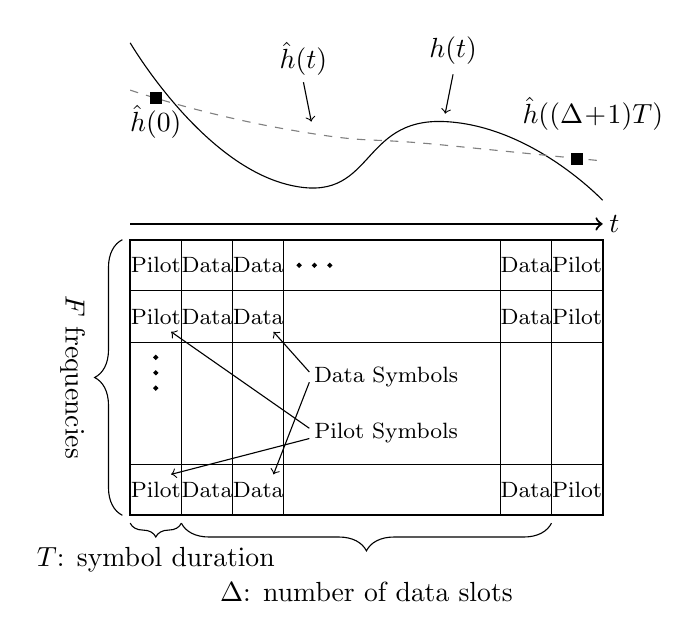
\begin{tikzpicture}[scale = 1]
  \def\x{0.65}
  \def\y{0.07}

  \draw[black, thick] (0,0) rectangle (6,3.5);

  \draw (\x,0) -- (\x,3.5);
  \draw (2*\x,0) -- (2*\x,3.5);
  \draw (3*\x,0) -- (3*\x,3.5);
  \draw (6-\x,0) -- (6-\x,3.5);
  \draw (6-2*\x,0) -- (6-2*\x,3.5);

  \draw (0, \x) -- (6, \x);
  \draw (0, 3.5-\x) -- (6, 3.5-\x);
  \draw (0, 3.5-2*\x) -- (6, 3.5-2*\x);

  \node at (\x/2, \x/2) {\footnotesize Pilot};
  \node at (\x/2, 3.5-\x/2) {\footnotesize Pilot};
  \node at (\x/2, 3.5-3*\x/2) {\footnotesize Pilot};

  \node at (3*\x/2, \x/2) {\footnotesize Data};
  \node at (3*\x/2, 3.5-\x/2) {\footnotesize Data};
  \node at (3*\x/2, 3.5-3*\x/2) {\footnotesize Data};

  \node at (5*\x/2, \x/2) {\footnotesize Data};
  \node at (5*\x/2, 3.5-\x/2) {\footnotesize Data};
  \node at (5*\x/2, 3.5-3*\x/2) {\footnotesize Data};

  \node at (6-3*\x/2, \x/2) {\footnotesize Data};
  \node at (6-3*\x/2, 3.5-\x/2) {\footnotesize Data};
  \node at (6-3*\x/2, 3.5-3*\x/2) {\footnotesize Data};

  \node at (6-\x/2, \x/2) {\footnotesize Pilot};
  \node at (6-\x/2, 3.5-\x/2) {\footnotesize Pilot};
  \node at (6-\x/2, 3.5-3*\x/2) {\footnotesize Pilot};

  \draw [->] (3.5*\x, 1.5*\x) -- (0.8*\x, 0.8*\x);
  \draw [->] (3.5*\x, 1.7*\x) -- (0.8*\x, 3.5-1.8*\x);
  \node at (5*\x, 1.6*\x) {\footnotesize Pilot Symbols};

  \draw [->] (3.5*\x, 2.6*\x) -- (2.8*\x, 0.8*\x);
  \draw [->] (3.5*\x, 2.8*\x) -- (2.8*\x, 3.5-1.8*\x);
  \node at (5*\x, 2.7*\x) {\footnotesize Data Symbols};

  \filldraw [black] (\x/2,3.5-2.3*\x) circle (0.7pt);
  \filldraw [black] (\x/2,3.5-2.6*\x) circle (0.7pt);
  \filldraw [black] (\x/2,3.5-2.9*\x) circle (0.7pt);

  \filldraw [black] (3.3*\x,3.5-\x/2) circle (0.7pt);
  \filldraw [black] (3.6*\x,3.5-\x/2) circle (0.7pt);
  \filldraw [black] (3.9*\x,3.5-\x/2) circle (0.7pt);

  \draw [decorate,decoration={brace,amplitude = 10pt}] (6-\x,-0.1) -- (\x,-0.1)
  node [black,midway,yshift=-25pt] {$\Delta$: number of data slots};
  \draw [decorate,decoration={brace,amplitude = 5pt}] (\x,-0.1) -- (0,-0.1)
  node [black,midway,yshift=-13pt] {$T$: symbol duration};


  \draw [decorate,decoration={brace,amplitude = 10pt}] (-0.1, 0) -- (-0.1,3.5)
  node [black,midway,xshift=-18pt] {\rotatebox{270}{$F$ frequencies}};

  \draw [->, thick] (0,3.7) -- (6,3.7);
  \node at (6.15, 3.7) {$t$};

  \draw plot [smooth, tension=1] coordinates { (0, 6) (2,4.2) (4,5) (6,4)};
  \draw [dashed, gray] plot [smooth, tension=1] coordinates { (0,5.4) (2,4.9) (4,4.7) (6,4.5)};

  \filldraw (\x/2-\y,5.3-\y) rectangle (\x/2+\y, 5.3+\y);
  \node at (\x/2, 5) {$\hat{\mx{h}}(0)$};
  \filldraw (6-\x/2-\y,4.52-\y) rectangle (6-\x/2+\y, 4.52+\y);
  \node at (6.2-\x/2, 5.1) {$\hat{\mx{h}}((\Delta\!+\!1)T)$};

  \draw [->] (4.1,5.6) -- (4,5.1);
  \node at (4.1, 5.9) {$\mx{h}(t)$};

  \draw [->] (2.2,5.5) -- (2.3,5);
  \node at (2.2, 5.8) {$\hat{\mx{h}}(t)$};
\end{tikzpicture}
\caption{Pilot (P) and data (D) symbols in the time-frequency domains of the system in the $(0,(\Delta+1)T)$ interval. The solid line above the
time-frequency resource grid represents the continuous time complex channel $\mx{h}(t)$, while the dashed line represents
the \ac{MMSE} channel estimate $\hat{\mx{h}}(t)$.
Notice that in each time slot of length $T$ all symbols are either pilot or
data symbols.}
\label{fig:Model}
\end{figure}

\begin{table}[t]
\caption{System Parameters}
\vspace{2mm}
\label{tab:notation}
\footnotesize
\begin{tabularx}{\columnwidth}{|X|X|}
\hline
\hline
\textbf{Notation} & \textbf{Meaning} \\
\hline
\hline
% Network layout
$K$ & Number of \ac{MU-MIMO} users \\
\hline
$N_r$ & Number of antennas at the BS \\
\hline
$F$ & Number of frequency channels used for pilot and data transmission within one slot \\
\hline
$\Delta$ & number of data slots in a data-pilot cycle \\
\hline
$\tau_p=F, \tau_d=\Delta F$ & Number of pilot/data symbols within a coherent set of subcarriers  \\
\hline
$\mx{s}\in \mathds{C}^{\tau_p \times 1}$ & Sequence of pilot symbols\\
\hline
$x$ & Data symbol \\
\hline
%$P_p, P, P_{\text{tot}}$ & Pilot power per symbol, data power per symbol, and total power budget  \\
$P_p, P$ & Pilot power per symbol, data power per symbol\\
\hline
$\mx{Y}^p(t) \in \mathds{C}^{N_r \times \tau_p}, y(t) \in \mathds{C}^{N_r}$ & Received pilot and data signal at time $t$, respectively  \\
\hline
% $\mx{N}, \mx{n}_d(t)$ & Additive white Gaussian noise at the received pilot and data signal, respectively \\
% \hline
$\alpha$ & Large scale fading between the mobile station and the base station \\
\hline
$\mx{C} \in \mathds{C}^{N_r \times N_r}$ & Stationary covariance matrix of the fast fading channel \\
\hline
$\mx{h}(t), \hat{\mx{h}}(t) \in \mathds{C}^{N_r}$ & Fast fading channel and estimated channel \\
% $\sigma_p^2 \mx{I}_{N_r}, \sigma_d^2 \mx{I}_{N_r}, \mx{C} \in \mathds{C}^{N_r \times N_r}$
% & Covariance of $\mx{N}$, $\mx{n}_d$, $\mx{h}(t)$, respectively \\
% \hline
\hline
$\bs{\varepsilon}(t) \in \mathds{C}^{N_r}, \bs{\Sigma} \in \mathds{C}^{N_r \times N_r}$
& Channel estimation error and its covariance matrix\\
\hline
%$\mx{G}, \mx{G}^\text{naive}, \mx{G}^\star$ & MU-MIMO receivers: generic, naive, and optimal, respectively. \\
$\mx{G}^\star$ & Optimal MU-MIMO receiver. \\
\hline
$f_D$ & Maximum Doppler frequency \\
\hline
$T$ & Slot duration \\
%\hline
%$\bs{\Lambda}_p$ & AWGN on the received pilot symbols at the \ac{BS} \\
\hline
\end{tabularx}
\end{table}

\subsection{Uplink Pilot Signal Model}
By extending the single antenna channel model of \cite{Savazzi:09},
each transmitting \ac{MS} uses a single time slot to send $F$ pilot symbols,
followed by $\Delta$ time slots, each of which containing $F$ data symbols according to Figure \ref{fig:Model}.
Each symbol is transmitted within a coherent time slot of duration $T$.
Thus, the total frame duration is $(1+\Delta) T$, such that each frame consists of 1 pilot
and $\Delta$ data time slots, which we will index with $i=1 \ldots \Delta$.
User-$k$ transmits each of the $F$ pilot symbols with transmit power $P_{p,k}$, and each data
symbol in slot-$i$ with transmit power $P_k(i),~k=1 \ldots K$.
To simplify notation, in the sequel we tag User-1, and will
drop index $k=1$ when referring to the tagged user.

Assuming that the coherence bandwidth accommodates at least $F$ pilot symbols,
this system allows to create $F$ orthogonal pilot sequences.
To facilitate spatial multiplexing
and \ac{CSIR} acquisition at the \ac{BS}, the \acp{MS} use orthogonal complex
sequences, such as shifted Zadoff-Chu sequences of length $\tau_p=F$, which we denote as:
\begin{align}
\mathbf{s} &\triangleq \left[s_1,...,s_{\tau_p}\right]^T \in \mathds{C}^{{\tau_p \times 1}},
\end{align}
whose elements satisfy %are scaled appropriately according to
$|s_i|^2 = 1$. %, for $i=1,..,\tau_p$ \cite{Sesia:11}.
% To enable spatial multiplexing, the length of the pilot sequences
% $\tau_p$ is chosen such that a maximum of $K$ users can be served simultaneously, implying that
% $\tau_p \geq K$ holds.
Under this assumption, the system can spatially multiplex $K\leq F$ \acp{MS}.
Focusing on the received pilot signal from the tagged user at the \ac{BS},
the received pilot signal takes the form of \cite{Fodor:21}:
\begin{align}
\mathbf{Y}^p(t)
&=
\alpha \sqrt{P_{p}}\mathbf{h}(t) \mathbf{s}^T +\mathbf{N}(t) ~~ \in \mathds{C}^{N_r \times \tau_p},
\label{eqn:received_training_seq}
\end{align}
where %we assume that
$\mathbf{h}(t) \in \mathds{C}^{N_r \times 1} \sim \mathcal{CN}(\mathbf{0},\mathbf{C})$, that is,
$\mathbf{h}(t)$ is a %circular symmetric
complex normal distributed column vector
with mean vector $\mathbf{0}$ and covariance matrix $\mx{C} \in \mathds{C}^{N_r \times N_r}$. % $\in \mathds{C}^{N_r \times N_r}$. %(of size $N_r$), %at all $t$ time instance,
Furthermore, $\alpha$ denotes
% propagation loss
large scale fading, $P_p$ denotes the pilot power of the tagged user,
and $\mathbf{N}(t)\in \mathds{C}^{N_r \times \tau_p}$
is the %spatially and temporally
\ac{AWGN} with element-wise variance $\sigma_p^2$.
It will be convenient to introduce $\mathbf{\tilde Y}^p(t)$ by stacking the columns of  $\mathbf{Y}^p(t)$ as:
\begin{align}
\mathbf{\tilde Y}^p(t)=\textbf{vec}\big(\mathbf{Y}^p(t)\big)=\alpha\sqrt{P_p} \mathbf{S} \mathbf{h}(t) +\mathbf{\tilde N}(t) ~\in \mathds{C}^{\tau_p N_r \times 1},
\label{eqn:received_training_seq2}
\end{align}
where $\textbf{vec}$ is the column stacking vector operator,
$\mathbf{\tilde Y}^p(t)$, $\mathbf{\tilde N}(t) \in \mathds{C}^{\tau_p N_r \times 1}$
and
$\mathbf{S} \triangleq \mathbf{s}\otimes \mathbf{I}_{N_r} \in \mathds{C}^{\tau_p N_r \times N_r}$
is such that $\mathbf{S}^H\mathbf{S}=\tau_p\mathbf{I}_{N_r}$,
where $\mathbf{I}_{N_r}$ is the identity matrix of size $N_r$.
\vspace{-2mm}
\subsection{Channel Model}
\vspace{-1mm}
% Consider a single block of $\Delta$ data symbols sent at time instances $iT$ for $i = 1\ldots \Delta$
% and a pilot symbol sent at time $0$ and subsequently at $(\Delta+1)T$.
In \eqref{eqn:received_training_seq},
the channel $\mx{h}(t)$ evolves continuously according to a multivariate complex stochastic process
with stationary covariance matrix $\mx{C}$.
That is, for symbol duration $T$, the channel ($\mx{h}(t)$) evolves according to the following \ac{AR} process:
\begin{align}
\label{eq:AR1}
\mx{h}(t+T) &= \mx{A} \mx{h}(t) + \bs{\vartheta}(t),
\end{align}
where the transition matrix of the \ac{AR} process is denoted by $\mx{A}$.
This \ac{AR} model has been commonly used to approximate Rayleigh fading channels in e.g. \cite{Baddour05}.
Equation \eqref{eq:AR1} implies that the autocorrelation function of the channel process is:
\begin{align}
\mathds{E}\left(\mx{h}(t)\mx{h}^H(t+iT)\right) &= \mx{C}\left(\mx{A}^H\right)^i, \quad \forall i.
\end{align}
%satisfies the following equation:
Consequently, the autocorrelation function of
the fast fading channel ($\mx{h}(t)$) is modelled as:
\begin{align}
\label{eq:autocorr}
\mx{R}(i) \triangleq
\mathds{E}\left(\mx{h}(t)\mx{h}^H(t+iT)\right) &= \mx{C} e^{\mx{Q}^H i T },
\end{align}
where matrix $\mx{Q}$ describes the correlation decay, such that:
\begin{align}
e^{\mx{Q}T} = \mx{A}.
\end{align}

Similarly, for user $k$,
\begin{align}
\label{eq:autocorrk}
\mx{R}_k(i) \triangleq
\mathds{E}\left(\mx{h}_k(t)\mx{h}_k^H(t+iT)\right) &= \mx{C}_k e^{\mx{Q}_k^H i T },
\end{align}

%We denote by $R(i) \triangleq cJ_0(2 \pi f_D i T)$ the correlation between the $i$-th element of
%the channel vectors that are $i \cdot T$ apart from each other in time.
% For the pilot channels we
In each pilot slot,
the \ac{BS} utilizes \ac{MMSE} channel estimation to obtain the channel estimate of each user, as it will be detailed in Section \ref{Sec:ChannelE}.
Without loss of generality, to simplify the notation, hereafter we assume that the time unit is $T$ and $iT=i$.

\begin{comment}
\begin{align}
\label{eq:LS}
\hat{\mx{h}}(t) &= \mx{h}(t) + \boldsymbol{\varepsilon}(t), \\
\boldsymbol{\varepsilon}(t) & \sim
%\mathcal{CN}\left(0,\frac{\boldsymbol{\Lambda}_p}{\alpha^2 F P_p} \right) \triangleq
\mathcal{CN}\left(0,\mx{\Sigma}\right)
\text{~with~} \mx{\Sigma} = \frac{\boldsymbol{\Lambda}_p}{\alpha^2 F P_p}
\end{align}
where $\mathcal{CN}\left(0,\mx{\Sigma}\right)$ is the $N_r$ dimensional complex normal distribution with mean $0$ and covariance matrix $\mx{\Sigma}$,  $\boldsymbol{\Lambda}_p$ is the covariance matrix of the \ac{AWGN} on the pilot symbols at the receiver
and $\alpha$ is the path loss between the \ac{MS} and the \ac{BS} \cite{Fodor:21}, which are assumed to be identical for all $F$ frequencies.
\end{comment}


\subsection{Data Signal Model}
When spatially multiplexing $K$ \ac{MU-MIMO} users,
the received data signal at the \ac{BS} at time $t$ is \cite{Fodor:21}:

\begin{align}
\mathbf{y}(t)
&=
\underbrace{\mathbf{\alpha} \mathbf{h}(t) \sqrt{P} x(t)}_{\text{tagged user}}
+ \underbrace{\sum_{k=2}^K \mathbf{\alpha}_{k} \mathbf{h}_k(t) \sqrt{P_{k}} x_{k}(t)}_{\text{co-scheduled MU-MIMO users}}
% \underbrace{\sum_{i \neq 1}^L \sum_{k=1}^K \mathbf{g}_{1,i,k} \sqrt{P_{i,k}} x_{i,k}}_{\text{Other cells}}
+\mathbf{n}_d(t),
%~~\in \mathds{C}^{N_r \times 1},
\label{eq:mumimo2}
\end{align}
\noindent where $\mathbf{y}(t)\in \mathds{C}^{N_r \times 1}$;
% and $\mathbf{\alpha}_{k} \mathbf{h}_k(t) \in \mathds{C}^{N_r \times 1}$
% denotes the channel vector,
and $x_k(t)$ denotes the transmitted data symbol of User-$k$
at time $t$ with transmit power $P_k$.
Furthermore, $\mathbf{n}_d(t)~\sim \mathcal{CN}\left(\mx{0},\sigma_d^2 \mathbf{I}_{N_r}\right)$
is the \ac{AWGN} at the receiver.
\vspace{-2mm}
\section{Channel Estimation}
\label{Sec:ChannelE}
In this section, we are interested in calculating the \ac{MMSE} estimation of the
channel in each slot $i$, based on received pilot signals, as a function of the frame
size corresponding to pilot spacing (see $\Delta$ in Figure \ref{fig:Model}).
Note that estimating the channel at the receiver can be based on
multiple received pilot signals both before and after the actual data slot $i$.
While using pilot signals that are received before data slot $i$ requires to
store the samples of the received pilot, using pilot signals that arrive after
data slot $i$ necessarily induces some delay in estimating the transmitted data symbol.
In the numerical section, we will refer to specific channel estimation strategies
as, for example, "1 before, 1 after" or "2 before, 1 after" depending on the number
of utilized pilot signals received prior to or following data slot $i$
for \ac{CSIR} acquisition.
In the sequel we use the specific case of "2 before, 1 after" to illustrate the
operation of the \ac{MMSE} channel estimation scheme,
that is when the receiver uses the pilot signals
$\mathbf{\tilde Y}^p(-\Delta-1)$, $\mathbf{\tilde Y}^p(0)$, and $\mathbf{\tilde Y}^p(\Delta+1)$
for \ac{CSIR} acquisition.
We are also interested in determining the distribution of the
resulting channel estimation error, whose covariance matrix, denoted by
$\mx{Z}(\Delta,i)$, will play an important role in subsequently determining
the deterministic equivalent of the \ac{SINR}.
\vspace{-2mm}
\subsection{\ac{MMSE} Channel Estimation and Channel Estimation Error}
As illustrated in Figure \ref{fig:Model},
in each data slot $i$, the \ac{BS} utilizes the \ac{MMSE} estimates of the channel
obtained in the neighboring pilot slots, for example at $(-\Delta-1)$, $0$ and $(\Delta+1)$, %according to \eqref{eqn:received_training_seq2}.
using the respective received pilot signals according to \eqref{eqn:received_training_seq2}, that is
$\mathbf{\tilde Y}^p\big((-\Delta-1)\big)$, $\mathbf{\tilde Y}^p(0)$ and $\mathbf{\tilde Y}^p\big((\Delta+1)\big)$, using the following lemma.

\begin{lem}
\label{lem:mmsechannel}	
The \textup{MMSE} channel estimator approximates the autoregressive fast fading channel in time slot $i$
based on the received pilots at $(-\Delta-1)$, $0$ and $(\Delta+1)$ as
\begin{align}
\label{eq:hmmse}
&\mathbf{\hat h}_{\textup{MMSE}}(\Delta,i)=
\mx{H^\star}(\Delta,i) \mathbf{\hat Y}^p(\Delta),
\end{align}
where
\begin{align*}
\mx{H^\star}(\Delta, i) = \frac{1}{\alpha \sqrt{P_p} \tau_p} \mx{E}(\Delta,i). \big(\mx{M}(\Delta)+\mx{\Sigma}_3\big)^{-1}.(\mx{s}^H\otimes \mx{I}_{3N_r}),
\end{align*}

$\mathbf{\hat Y}^p(\Delta) \triangleq \begin{bmatrix}
\mathbf{\tilde Y}^p((-\Delta-1)) \\
\mathbf{\tilde Y}^p(0) \\
\mathbf{\tilde Y}^p((\Delta+1))
\end{bmatrix}$~~and~~$\mx{\Sigma}_3\triangleq \frac{\sigma_p^2}{\alpha^2P_p \tau_p} \mx{I}_{3N_r}$,
\begin{align}
\label{eq:E}
\mx{E}(\Delta,i) &\triangleq
\begin{bmatrix}
\mx{R}(\Delta \!+\! 1 \!+\! i) & \mx{R}(i) &
\mx{R}(\Delta \!+\! 1 \!-\! i)
\end{bmatrix},
\\
\label{eq:M}
\mx{M}(\Delta) &\triangleq
\begin{bmatrix}
\mx{C} & \mx{R}(\Delta \!+\! 1) & \mx{R}(2\Delta \!+\! 2)  \\
\mx{R}^H(\Delta \!+\! 1) & \mx{C} & \mx{R}(\Delta \!+\! 1) \\
\mx{R}^H(2\Delta \!+\! 2) & \mx{R}^H(\Delta \!+\! 1) & \mx{C}\\
\end{bmatrix}.
\end{align}

\end{lem}

\begin{proof}
The \ac{MMSE} channel estimator aims at minimizing the \ac{MSE} between the channel estimate
$\mathbf{\hat h}_{\textrm{MMSE}}(\Delta, i) = \mathbf{H}^\star(\Delta, i) \mathbf{\hat Y}^p(\Delta)$ and the channel $\mathbf{h}(i)$, that is
\begin{align}
\mathbf{H^\star}(\Delta, i)= \text{arg} \min_{\mathbf{H}} \mathds{E}_{\mathbf{h},\mathbf{n}}\{ ||\mathbf{H} \mathbf{\hat Y}^p(\Delta) - \mathbf{h}(i)||^2 \}.
\end{align}
The solution of this quadratic optimization problem is
$\mathbf{H^\star}(\Delta, i)= \mx{a}(\Delta, i)^H \mx{F}^{-1}(\Delta)$
with
\begin{align}
\label{eq:Fandb}
\mx{F}(\Delta) &\triangleq \mathds{E}_{\mathbf{h},\mathbf{n}}\left(\mx{\hat Y}^p(\Delta) \left(\mx{\hat Y}^p(\Delta)\right)^H\right), \\
\mx{a}(\Delta, i) &\triangleq \mathds{E}_{\mathbf{h},\mathbf{n}}\left( \mx{\hat Y}^p(\Delta) \mx{h}^{H}(i)\right).
\end{align}
Let
\begin{align}
\mx{\bar h}(\Delta) \triangleq \begin{bmatrix}
\mx{h}((-\Delta-1)) \\
\mx{h}(0) \\
\mx{h}((\Delta+1))
\end{bmatrix} \nonumber
\end{align}
and
\begin{align}
\mx{\tilde{\bar{N}}}(\Delta) \triangleq \begin{bmatrix}
\mx{\tilde{N}}((-\Delta-1)) \\
\mx{\tilde{N}}(0) \\
\mx{\tilde{N}}((\Delta+1))
\end{bmatrix}.
\end{align}
Using $\mx{\bar h}(\Delta)$, we have
\begin{align}
\begin{bmatrix}
\mx{S}\mx{h}((-\Delta-1)) \\
\mx{S}\mx{h}(0) \\
\mx{S}\mx{h}((\Delta+1))
\end{bmatrix}=
\begin{bmatrix}
\mx{S}  & \mx{0} & \mx{0} \\
\mx{0} & \mx{S}  & \mx{0} \\
\mx{0} & \mx{0} & \mx{S}
\end{bmatrix}\mx{\bar h}(\Delta)
\nonumber \\
~~~~~~~~= (\mx{I}_3\otimes\mx{S}) \mx{\bar h}(\Delta)=  (\mx{s}\otimes \mx{I}_{3N_r}) \mx{\bar h}(\Delta).
\end{align}
Since $\mx{\bar h}(\Delta)$ and $\mx{\tilde{\bar{N}}}(\Delta)$ are independent and
\begin{align}
\mathds{E}_{\mathbf{h},\mathbf{n}}(\mx{\bar h}(\Delta)\mx{\bar h}^H(\Delta))&=\mx{M}(\Delta),\\
\mathds{E}_{\mathbf{h},\mathbf{n}}(\mx{h}(i)\mx{\bar h}^H(\Delta))&=\mx{E}(\Delta,i).
\end{align}
Therefore, for $\mx{F}(\Delta)$ and $\mx{a}(\Delta,i)$, we have
\begin{align*}
\mx{F}(\Delta) &=
%\mathds{E}_{\mathbf{h},\mathbf{n}}\left(\mx{\tilde{\bar{Y}}}^p\mbox{$\mx{\tilde{\bar{Y}}}^p$}^H\right)\\&=
\mathds{E}_{\mathbf{h},\mathbf{n}}
\left(\left(\alpha\sqrt{P_p} (\mx{I}_3\otimes\mx{S}) \mx{\bar{h}}(\Delta) +\mx{\tilde{\bar{N}}}(\Delta)\right)\right.\nonumber \\
&~~~~~~~~~~~~\cdot \left.\left(\alpha\sqrt{P_p} (\mx{I}_3\otimes\mx{S}) \mx{\bar{h}}(\Delta) +\mx{\tilde{\bar{N}}}(\Delta)\right)^H\right)\\
&=\alpha^2P_p(\mx{I}_3\otimes\mx{S})\mx{M}(\Delta)\left(\mx{I}_3\otimes\mx{S}^H\right)+ \sigma_p^2 \mathbf{I}_{3N_r\tau_p},\\
\mx{a}(\Delta, i) &= \mathds{E}_{\mathbf{h},\mathbf{n}}\left( \mx{\hat Y}(\Delta) \mx{h}^{H}(i)\right) \\
&=\mathds{E}_{\mathbf{h},\mathbf{n}}
\left(\left(\alpha\sqrt{P_p} (\mx{I}_3\otimes\mx{S}) \mx{\bar{h}}(\Delta) +\mx{\tilde{\bar{N}}}(\Delta)\right)
\mx{h}^{H}(i)\right)\\
&= \alpha\sqrt{P_p} ~(\mx{I}_3\otimes\mx{S})~\mx{E}(\Delta,i)^T,
\end{align*}
which yields Lemma \ref{lem:mmsechannel}.
\end{proof}

The \ac{MMSE} estimate of the channel is then expressed as:
\begin{align}
\nonumber
&\mathbf{\hat h}_{\textrm{MMSE}}(\Delta, i)=\mathbf{H^\star}(\Delta, i) \mathbf{\hat Y}^p(\Delta) ~~~~ \\
&~~~~=\mathbf{H^\star}(\Delta, i)
\left(\alpha\sqrt{P_p} (\mx{I}_3\otimes\mx{S}) \mx{\bar{h}}(\Delta) +\mx{\tilde{\bar{N}}}(\Delta)\right)
\nonumber
\\
&~~~~=
\frac{1}{\alpha\sqrt{P_p} \tau_p}
\mx{E}(\Delta, i) \left(   \mx{M}(\Delta) + \mx{\Sigma}_{3} \right)^{-1}
\nonumber
\\&~~~~~~~~~~.
\left(\alpha\sqrt{P_p} \tau_p \mx{\bar{h}}(\Delta) + \left(\mx{I}_3 \otimes \mx{S}^H\right) \mx{\tilde{\bar{N}}}(\Delta)\right).
\label{eq:MMSEt}
\end{align}

Next, we are interested in deriving the distribution of the estimated channel and
the channel estimation error, since these will be important for understanding the
impact of pilot spacing on the achievable \ac{SINR} and spectral efficiency of
the \ac{MU-MIMO} system. To this end, the following two corollaries of
Lemma \ref{lem:mmsechannel} and \eqref{eq:MMSEt} will be important in the sequel.
\begin{cor}
\label{cor:rmmse}	
The estimated channel $\mathbf{\hat h}_{\textup{MMSE}}(\Delta, i)$ is a circular symmetric complex normal distributed vector
$\mathbf{\hat h}_{\textup{MMSE}}(\Delta, i) \sim %\mathcal{CN}(\mathbf{0},\mathbf{R}_{\textup{MMSE}}(\Delta, i))$,
\mathcal{CN}\Big(\mathbf{0},\mathbf{\hat \Phi}_{\textup{MMSE}}(\Delta, i)\Big)$,
with
\begin{align}
\label{eq:rmmse}
\mathbf{\hat \Phi}_{\textup{MMSE}}(\Delta, i) \triangleq
& \mathds{E}_{\mathbf{h},\mathbf{n}} \{\mathbf{\hat h}_{\textup{MMSE}}(\Delta, i) \mathbf{\hat h}_{\textup{MMSE}}^H(\Delta, i)\}
 \nonumber \\
=& \mx{E}(\Delta, i) \big(\mx{M}(\Delta)+\mx{\Sigma}_3\big)^{-1} \mx{E}(\Delta, i)^H.
\end{align}

\end{cor}

\begin{proof}
Equation \eqref{eq:rmmse} follows directly from \eqref{eq:MMSEt}.	
\end{proof}

An immediate consequence of Corollary \ref{cor:rmmse}
is the following corollary regarding the covariance of the channel estimation
error, as a function of pilot spacing.
\begin{cor}
\label{Cor:ChEstError}
The channel estimation error in slot $i$, $\mx{\hat{h}}_{\textup{MMSE}}(\Delta, i)-\mx{h}(\Delta, i)$,
is complex normal distributed with zero mean vector and
covariance matrix given by:
\begin{align}
\label{eq:Z}
\mx{Z}(\Delta, i) \triangleq  \mx{C} -
\mx{E}(\Delta, i) \big(\mx{M}(\Delta)+\mx{\Sigma}_3\big)^{-1}
\mx{E}(\Delta, i)^H.
\end{align}
\end{cor}

In the following section we will calculate the \ac{SINR} of the received data symbols.
For simplicity of notation, we use $\mx{\hat h}_{\textup{MMSE}}(\Delta, i)=\mx{\hat h}(\Delta, i)$, and  introduce
$$\mx{b}(\Delta, i) \triangleq \alpha\sqrt{P(i)}\mx{\hat{h}}(\Delta, i)$$
with covariance matrix
\begin{align}
\label{eq:Phi}
\bs{\Phi}(\Delta, i) & \triangleq
\mathds{E}\left( \mx{b}(\Delta, i)\mx{b}^H(\Delta, i) \right)  \nonumber \\
&=\mathds{E}\left( \Big(\alpha\sqrt{P(i)} \mx{\hat{h}}(\Delta, i) \Big)\Big(\alpha\sqrt{P(i)} \mx{\hat{h}}(\Delta, i) \Big)^H  \right)  \nonumber \\
&=\alpha^2P(i)(\mx{C}-\mx{Z}(\Delta, i)).
\end{align}
% \dg{For consistency, shouldn't we use $P_i$ instead of $P(i)$?}
\subsection{Summary}

This section derived the \ac{MMSE} channel estimator (Lemma \ref{lem:mmsechannel})
that uses the received pilot signals
both before and after a given data slot $i$ and depends on the frame size $\Delta$ (pilot spacing).
As important corollaries of the channel estimation scheme, we established the distribution
of both the estimated channel (Corollary \ref{cor:rmmse})
and the associated channel estimation error in each data
slot $i$ (Corollary \ref{Cor:ChEstError}), as functions of both the employed pilot spacing and pilot power. These
results serve as a starting point for deriving the achievable \ac{SINR} and spectral
efficiency.

\section{\ac{SINR} Calculation}
\label{Sec:SINR}

\subsection{Instantaneous \ac{SINR}}
We start with recalling an important lemma from \cite{Fodor:22}, which calculates the instantaneous \ac{SINR}
in an \ac{AR} fast fading environment
when the \ac{BS} uses the \ac{MMSE} estimation of the fading channel, and employs the optimal linear
receiver:
\begin{align}
\label{eq:Gstar2}
\mx{G}^\star(\Delta, i) &=
% \textup{arg} \min_{\mx{G}} \textup{MSE}\left(\mx{G},\mx{\hat H}(t), \mx{\hat H}(t-1)\right)
\mx{b}^H(\Delta,i) \mx{J}^{-1}(\Delta,i),
\end{align}
where $\mx{J}(\Delta, i) \in \mathds{C}^{N_r \times N_r}$
is defined as
\begin{align}
%\label{eq:A3}
\nonumber
\mx{J}(\Delta, i)
&\triangleq
\sum_{k=1}^K  \mx{b}_k(\Delta, i) \mx{b}_k^H(\Delta, i) + \bs{\beta}(\Delta, i),
\end{align}
where
\begin{align}
\label{eq:beta}
\bs{\beta}(\Delta, i) \triangleq \sum_{k=1}^K \alpha_k^2 P_k  \mx{Z}_k(\Delta, i) + \sigma^2_d \mx{I}_{N_r}.
\end{align}
%and $\mx{I}$ is the identity matrix of size $N_r$.

When using the above receiver, which minimizes the \ac{MSE} of the received data symbols in the
presence of channel estimation errors, the following result from \cite{Fodor:22} will be useful in the sequel:
\begin{lem}[See \cite{Fodor:22}, Lemma 3]
Assume that
the receiver employs \textup{\ac{MMSE}} symbol estimation,
that is it employs the optimal linear receiver $\mx{G}^\star(\Delta, i)$ given in \eqref{eq:Gstar2}. %and the instantaneous channel estimates,
Then the instantaneous \textup{\ac{SINR}} of the estimated data symbols of the tagged user,
$\gamma(\Delta, i)$ %\Big(\mathbf{G}^\star, \hat{\mathbf{H}}(t),\hat{\mathbf{H}}(t-1)\Big)$
is given as:
% the instantaneous \textup{\ac{SINR}} of the data symbols, can be expressed as:
%
\begin{equation}
\label{eq:lemma2Eq}
\gamma(\Delta, i) %\Big(\mathbf{G}^\star(t), \hat{\mathbf{H}}(t),\hat{\mathbf{H}}(t-1)\Big)
=
\mx{b}^H(\Delta, i) \mathbf{\bar{J}}^{-1}(\Delta, i) \mx{b}(\Delta, i),
\end{equation}
where
\vspace{-1mm}
\begin{equation}
\mathbf{\bar{J}}(\Delta, i) \triangleq \mathbf{J}(\Delta, i)- \mx{b}(\Delta, i)\mx{b}^H(\Delta, i).
\end{equation}
\end{lem}
\begin{comment}
Using the \ac{MMSE} estimate $\bar{\mx{h}}(i) = \mx{E}(i) \mx{\hat{\bar{h}}}(\Delta)$ of the channel $\mx{h}(i)$,
we can calculate the \ac{SINR} of the estimated data symbol sent at time $i$ when the \ac{BS} employs an optimal linear receiver as provided in \cite{Fodor:22}.
Lemma 2 in \cite{Fodor:22} shows that when $K$ \acp{MS} enumerated $k = 1 \ldots K$ transmit data signals
through channels $\mx{h}_k$ with \ac{MMSE} estimates
$\bar{\mx{h}}_k$, estimation error covariance $\mx{Z}_k$, path losses $\alpha_k$,
and employing transmit powers $P_k$, the \ac{SINR} of the estimated data symbol of user $k$, $\hat x = \mx{G}\mx{y}$:

\begin{align}
    \gamma_k = \alpha_k^2 P_k \bar{\mx{h}}_k^H \left( \sum_{l \neq k}^K \alpha_l^2 P_l \bar{\mx{h}}_l\bar{\mx{h}}_l^H
    + \sum_{l = 1}^K \alpha_l^2 P_l \mx{Z}_l + \sigma_d^2 \mx{I} \right)^{-1}\bar{\mx{h}}_k,
\end{align}

where $\sigma_d^2$ is the variance of the \ac{AWGN} on the data signal.
Applying this formula on the previous section, where the data symbol of User-$k$, in data time slot $i$ is transmitted through the channel $\mx{h}_k(iT)$,
with \ac{MMSE} estimate $\bar{\mx{h}}_k(iT) = \mx{E}_k(i) \bs{\zeta}_k(\Delta)$ and channel covariance matrix $\mx{Z}(i)$
the \ac{SINR} of the estimated data symbol sent by User-$k$ is given by
\end{comment}
For the \ac{AR} fading case considered in this paper,
based on the definitions of $\mx{b}(\Delta, i)$, $\mx{J}(\Delta, i)$ and $\mx{\bar{J}}(\Delta, i)$,
the instantaneous \ac{SINR} of the tagged user is then expressed as:
\begin{align}
\gamma(i) &  =  \mx{b}^H(\Delta, i) \mathbf{\bar{J}}^{-1}(\Delta, i) \mx{b}(\Delta, i)
  \nonumber\\
 &=
\textup{tr}\left( \mx{b}(\Delta, i)\mx{b}^H(\Delta, i) \mathbf{\bar{J}}^{-1}(\Delta, i) \right).
\end{align}

\subsection{Slot-by-Slot Deterministic Equivalent of the \ac{SINR} as a Function of Pilot Spacing $\Delta$}
We can now prove the following important proposition that gives the asymptotic deterministic equivalent
of the instantaneous \ac{SINR} in data slot $i$, $\bar{\gamma}(\Delta, i)$, when the number of antennas $N_r$ approaches infinity.
This asymptotic equivalent \ac{SINR} gives a good approximation of averaging the instantaneous \ac{SINR} of the tagged user \cite{Wagner:2012, Hoydis:13, Fodor:22}.

\begin{prop}
\label{Prop:SINR}
% According to this theorem, for User-$1$ the \ac{SINR} is given by
The asymptotic deterministic equivalent \ac{SINR} of the tagged user in data slot $i$ can be calculated as:
\begin{align}
\label{eq:hoydis1}
\bar{\gamma}(\Delta, i) &= \textup{tr}\Big( \bs{\Phi}(\Delta, i)\mx{T}(\Delta, i)  \Big),
\end{align}
where $\mx{T}(\Delta, i)$ is defined as: %given by
\begin{align}
\label{eq:hoydis2}
\mx{T}(\Delta, i) \triangleq \left( \sum_{m = 2}^{K} \frac{\bs{\Phi}_m(\Delta, i)}{1 + \delta_m(\Delta, i)} + \bs{\beta}(\Delta, i) \right)^{-1},
\end{align}
and $\delta_m(\Delta, i)$ are the solutions of the following system of $K$ equations
\begin{align}
\label{eq:hoydis3}
\delta_m(\Delta, i) &= \textup{tr}\left(\bs{\Phi}_m(\Delta, i)
\left( \sum_{l = 2}^{K} \frac{\bs{\Phi}_l(\Delta, i)}{1 + \delta_l(\Delta, i)} + \bs{\beta}(\Delta, i)  \right)^{-1} \right)
\end{align}
for $\forall m = 1, \ldots, K$.
\end{prop}
The above system of $K$ equations gives the deterministic equivalent of the \ac{SINR} of the tagged user,
and a different set of $K$ equations must be used for each user.
\begin{proof}
The $\mx{b}_k(\Delta, i)$ vectors are independent for $k = 1 \ldots K$,
and the covariance matrix of $\mx{b}_k(\Delta, i)$ is $\bs{\Phi}_k(\Delta, i)$
(c.f. \eqref{eq:Phi}).
We can then express the expected value of the \ac{SINR} of the tagged user as follows:
\begin{align}
\label{eq:gammaB}
& \bar{\gamma}(\Delta, i) \triangleq \mathds{E}\Big(\gamma(\Delta, i)\Big)   \\
&= \mathds{E}\left( \textup{tr}\left( \bs{\Phi}(\Delta, i)  \left( \sum_{l = 2}^K  \mx{b}_l(\Delta, i) \mx{b}_l^H(\Delta, i)  +\bs{\beta}(\Delta, i) \right)^{\!\!-1}  \right) \right).
\nonumber
\end{align}
%We proceed
The proposition is established
by invoking Theorem \ref{thm:upperbound} in \cite{Wagner:2012}, which is applicable in multiuser systems and
% Theorem \ref{thm:upperbound} in \cite{Wagner:2012}
gives the value of the deterministic equivalent of $\bar{\gamma}(\Delta, i)$
implicitly using a system of $K$ equations and noticing that
$\bar{\gamma}(\Delta, i) = \delta_1(\Delta, i)$, since $\delta_1(\Delta, i)=\textup{tr}\big( \bs{\Phi}(\Delta, i) \mx{T}(\Delta, i)\big)$ according to \eqref{eq:hoydis3}.
\end{proof}

\subsection{Summary}
This section established the instantaneous slot-by-slot \ac{SINR} of a tagged user ($\bar \gamma(i)$) of a \ac{MU-MIMO} system operating over %continuous time
a fast fading channels modelled as \ac{AR} processes,
by applying our previous result obtained for discrete-time \ac{AR} channels
reported in \cite{Fodor:21}.
Next, we invoked Theorem \ref{thm:upperbound} in \cite{Wagner:2012}, to establish the deterministic
equivalent \ac{SINR} for each slot, as a function of the frame size (pilot spacing) $\Delta$, see Proposition \ref{Prop:SINR}.
These results serve as a basis for formulating the pilot spacing optimization problem over the frame size and pilot power as optimization variables.

\section{Pilot Spacing and Power Control}
\label{Sec:PilotSpacing}
In this section, we study the impact of pilot spacing and power control on the achievable \ac{SINR}
and the \ac{SE} of all users in the system.
The asymptotic \ac{SE} of the $i$-th data symbol of user $k$ is
\begin{align}
\label{eq:SE}
\text{SE}_k(\Delta, i) \triangleq \log\Big(1 + \bar{\gamma}_k(\Delta, i)\Big),
\end{align}
where $\bar{\gamma}_k(\Delta, i)$ denotes the average \ac{SINR} of  user $k$ when sending the $i$-th data symbol, and when $\Delta$ data symbols are sent between every pair of pilot symbols.
Consequently, the %information rate
average \ac{SE}
of  user $k$ over the $(\Delta+1)$ slot long frame is
\begin{align}
\frac{\sum_{i=1}^{\Delta}\text{SE}_k(\Delta, i)}{\Delta + 1},
\end{align}
which can be optimized over $\Delta$.
More importantly, %the sum information rate
the aggregate average \ac{SE}
of the \ac{MU-MIMO} system for the $K$ users can be expressed as:
\begin{align}
\text{SE}(\Delta) = \frac{\sum_{k=1}^K \sum_{i=1}^{\Delta}\text{SE}_k(\Delta,i)}{\Delta + 1}.
\label{eq:multiopt}
\end{align}


\subsection{An Upper Bound of the Deterministic Equivalent \ac{SINR} and the \ac{SE}}

Let us assume that $\mx{Q}_k=q_k \mx{I}_{N_r}$, that is the
channel vector $\mx{h}_k(t)$ consists of independent \ac{AR} processes in the spatial domain, implying that:
\begin{align}
\label{eq:r1}
\mx{R}_k(i) \triangleq
\mathds{E}\left(\mx{h}_k(t)\mx{h}_k^H(t+i)\right) &= \mx{C}_k e^{q_k^* i},
\end{align}
where $q_k$ is a scalar, $q_k^*$ denotes complex conjugation, and let $\bar{q}_k\triangleq Re(q_k)<0$.

Note that the exponential approximation of the autocorrelation function of the fast fading process expressed
in \eqref{eq:r1} is related to the Doppler frequency of Rayleigh fading through:
\begin{align}
\label{eq:RayleighApprox}
\underbrace{\mx{C}J_0(2 \pi f_D i)}_{\text{True autocorrelation of Rayleigh fading}} &\approx \mx{R}(i),
\end{align}
where $J_0(.)$ is the zeroth order Bessel function \cite{Wang:03}.
Based on the exponential approximation of this Rayleigh fading process in \eqref{eq:r1}, the Doppler frequency of the approximate model is obtained from $2 \pi f_D i = Re(q_k^* i)$, i.e. $f_D = 2 \pi/\bar{q}_k$.

To optimize \eqref{eq:multiopt}, we first find an upper bound of $\text{SE}_k(\Delta,i)$
via an upper bound of $\bar{\gamma}_k(\Delta, i)$.
To simplify the notation, the following discussion refers to the tagged user, and later we utilize that the same relations hold for all users.
We introduce the following upper bound of $\bar{\gamma}(\Delta, i)$:
\begin{align}
\label{eq:upper}
\bar{\gamma}^{(u)}(\Delta, i) \!&\triangleq \textup{tr}\!\left(\! \bs{\Phi}^{(u)}(\Delta, i)  \left(\sum_{l = 1}^K \!\alpha_l^2 P_l \mx{Z}^{(u)}_l(\Delta, i) \!+\! \sigma_d^2 \mx{I_{N_r}}\right)^{\!\!\!-1}  \!\right)\!,
\end{align}
where $\mx{Z}^{(u)}(\Delta, i)$ and $\bs{\Phi}^{(u)}(\Delta, i)$ are given by
\begin{align}
\label{eq:zu}
\mx{Z}^{(u)}(\Delta, i) &\triangleq \mx{C} - \rho(\Delta, i) \mx{C} \left(\eta  \mx{C} + \bs{\Sigma} \right)^{-1} \mx{C},  \\
\label{eq:phiu}
\bs{\Phi}^{(u)}(\Delta, i) &\triangleq \alpha^2 P \rho(\Delta, i) \mx{C} \left( \eta \mx{C} + \bs{\Sigma} \right)^{-1} \mx{C},
\end{align}
with $\eta$ being a constant, $\mx{\Sigma}\triangleq \frac{\sigma_p^2}{\alpha^2P_p \tau_p} \mx{I}_{N_r}$ and
\begin{align}
\label{eq:rho}
%\mx{\Sigma} &\triangleq \frac{\sigma_p^2}{\alpha^2P_p %\tau_p} \mx{I}_{N_r} \\
\rho(\Delta, i) &\triangleq e^{2\bar{q} (\Delta + 1 + i)} + e^{2\bar{q}  i} + e^{2\bar{q} (\Delta + 1 - i)}.
\end{align}

\begin{thm}
\label{thm:upperbound}
If $\bar{q}<0$ and
\begin{align}
\label{eq:etacond}
0<\eta<\frac{1}{2}\left(2+a^2-a\sqrt{8+a^2}\right),
\end{align}
with $a\triangleq e^{2\bar{q}}$
then  $\bar{\gamma}(\Delta, i)\leq \bar{\gamma}^{(u)}(\Delta, i)$.
\end{thm}
%\overset{(a)}{=}
\begin{proof}
We prove the theorem based on the following inequalities
\begin{align}
\bar{\gamma}(\Delta, i)
&\overset{(a)}{\leq}
\textup{tr}\left( \bs{\Phi}(\Delta, i) \bs{\beta}(\Delta, i)^{-1} \right) \nonumber \\
&\overset{(b)}{\leq}
   \textup{tr}\left( \bs{\Phi}^{(u)}(\Delta, i) \bs{\beta}(\Delta, i)^{-1} \right)
\overset{(c)}{\leq}
   \bar{\gamma}^{(u)}(\Delta, i),  \label{eq:gammabound}
\end{align}
which are proved in consecutive lemmas.
\end{proof}

%The following properties of positive semi-definite matrices are essential to prove the theorem.
\begin{lem}
\label{lem:AB}
Let $\mx{A}$, $\mx{B}$ and $\mx{C}$ be positive definite matrices and $\mx{D}$ be any matrix, such that $\mx{A} \preceq \mx{B}$ (i.e. $\mx{B}-\mx{A}$ is a positive semidefinite matrix), then
\begin{align}
\label{eq:ABinv}
\mx{A}^{-1} &\succeq \mx{B}^{-1},
\\
\label{eq:AB3}
\textup{tr}\left( \mx{D}^H \mx{A} \mx{D} \right) &\leq \textup{tr}\left(\mx{D}^H \mx{B} \mx{D} \right) \\
\label{eq:AB1}
\textup{tr}\left( \mx{A} \mx{C} \right) &\leq \textup{tr}\left(\mx{B} \mx{C} \right)
\\
\label{eq:AB2}
\textup{tr}\left( \mx{C} \mx{A}^{-1} \right) &\geq \textup{tr}\left( \mx{C} \mx{B}^{-1} \right).
\end{align}
\end{lem}
\begin{proof}
$\mx{A}^{-1} \succeq \mx{B}^{-1}$ is given in \cite[p. 495, Corollary 7.7.4(a)]{Horn2013}.
\eqref{eq:AB3} follows from the fact that $\mx{D}^H (\mx{B}-\mx{A}) \mx{D}$ is a positive semidefinite matrix since $\mx{B}-\mx{A}$ is a positive semidefinite matrix and
for any $\mx{x}$
\begin{align}
\mx{x}^H \mx{D}^H (\mx{B}-\mx{A}) \mx{D} \mx{x} = \mx{y}^H (\mx{B}-\mx{A}) \mx{y} \geq 0
\end{align}
where $\mx{y} \triangleq \mx{D} \mx{x}$.
Let $\mx{C}=\mx{D}^H \mx{D}$ be the Cholesky decomposition of $\mx{C}$ then
\eqref{eq:AB1} and \eqref{eq:AB2} follows from \eqref{eq:AB3}, by utilizing the cyclic property of the trace operator.
\end{proof}

\begin{lem}
\label{lem:beta}
For $\bar{q}<0$ and $\eta$ satisfying \eqref{eq:etacond},
the following relation holds
\begin{align}
&\mx{E}(\Delta, i) \big(\mx{M}(\Delta,i)+\mx{\Sigma}_3\big)^{-1} \mx{E}(\Delta, i)^H
\nonumber \\&
~~~~~~~~~~~~~~\preceq \rho(\Delta, i) \mx{C} \left( \eta \mx{C} \!+\! \bs{\Sigma} \right)^{-1} \mx{C}
\label{eq:mrel}
\end{align}
\end{lem}
\begin{proof}
The proof is in Appendix \ref{Sec:L4}.
\end{proof}

Having prepared with Lemma \ref{lem:AB} and Lemma \ref{lem:beta}, we can prove the (a), (b) and (c) inequalities in \eqref{eq:gammabound} by Lemma \ref{lem:det} ((a) part) and Lemma \ref{lem:ineq} ((b) and (c) parts) as follows.
\begin{lem}
\label{lem:det}
The deterministic equivalent \ac{SINR} of the tagged user satisfies
\begin{align}
& \bar{\gamma}(\Delta, i) \leq   \textup{tr}\left( \bs{\Phi}(\Delta, i) \bs{\beta}(\Delta, i)^{-1} \right).
\nonumber
\end{align}
\end{lem}
\begin{proof}
The proof is in Appendix \ref{Sec:L5}.
\end{proof}

%We can now state the following lemma, which completes the proof of inequality \eqref{eq:gammabound} by proving the (b) and (c) inequalities of \eqref{eq:gammabound}.
\begin{lem}
\label{lem:ineq}
When the conditions of Theorem \ref{thm:upperbound} hold, we have
\begin{align}
 \textup{tr}\left( \bs{\Phi}(\Delta, i) \bs{\beta}(\Delta, i)^{-1} \right) &\leq
\textup{tr}\left( \bs{\Phi}^{(u)}(\Delta, i) \bs{\beta}(\Delta, i)^{-1} \right)
\label{eq:gammabound1}
\\
  \textup{tr}\left( \bs{\Phi}^{(u)}(\Delta, i) \bs{\beta}(\Delta, i)^{-1} \right)
&\leq \bar{\gamma}^{(u)}(\Delta, i).
\label{eq:gammabound2}
\end{align}
\end{lem}

\begin{proof}
When the conditions of Theorem \ref{thm:upperbound} hold,
Lemma \ref{lem:beta} implies that
 $\bs{\Phi}(\Delta, i)\preceq \bs{\Phi}^{(u)}(\Delta, i)$
 and
$\mx{Z}(\Delta, i) \succeq \mx{Z}^{(u)}(\Delta, i)$.
Using the first relation and %Lemma \ref{lem:AB}
the Lemma \ref{lem:AB}
gives \eqref{eq:gammabound1},
while using the second relation and Lemma \ref{lem:AB} gives \eqref{eq:gammabound2}.
\end{proof}

%\gf{\it GF16: Maybe introducing $\bs{\beta}^{(u)}(\Delta,i) \succeq \bs{\beta}(\Delta,i)$ would simplify the presentation of the proof.}

\subsection{Useful Properties of the Upper Bounds on the Deterministic Equivalent \ac{SINR} and Overall System Spectral Efficiency}

Theorem \ref{thm:upperbound} is useful, because it establishes an upper bound,
denoted by $\bar{\gamma}^{(u)}(\Delta, i)$,
of the deterministic equivalent of the \ac{SINR},
$\bar{\gamma}(\Delta, i)$.

To use the $\bar{\gamma}^{(u)}(\Delta, i)$ upper bound for limiting the search space for an optimal $\bar{\gamma}(\Delta, i)$ in Section \ref{Sec:Alg}, we need the following properties of the upper bound.

%Clearly, the deterministic equivalent \ac{SINR} is not necessarily a monotonic function of $\Delta$. However, we can now prove that the upper bound established by Theorem \ref{thm:upperbound} is monotonically decreasing in $\rho$, and tends to zero as $\rho \rightarrow 0$, which properties will turn out to imply some useful properties of the overall spectral efficiency, as we will see later in Proposition \ref{UpperB2}.


\begin{prop}
\label{UpperB1}
The $\bar{\gamma}^{(u)}(\Delta, i)$ upper bound has the following properties:
$\partial \bar{\gamma}^{(u)}(\Delta, i) / \partial \rho(\Delta, i) \geq 0$ and $\rho(\Delta, i) \rightarrow 0 \Rightarrow \bar{\gamma}^{(u)}(\Delta, i) \rightarrow 0$.
\end{prop}
\begin{proof}
The proof is in Appendix \ref{Sec:P2}.
\end{proof}

Similarly, the SINR of user $k$ satisfies the inequality
$\bar{\gamma}_k(\Delta, i) \leq \bar{\gamma}_k^{(u)}(\Delta, i)$
where $\bar{\gamma}_k^{(u)}(\Delta, i)$ is defined in a similar way as $\bar{\gamma}_1^{(u)}(\Delta, i)$.
The $\bar{\gamma}_k^{(u)}(\Delta, i)$ upper bound is such that
$\partial \bar{\gamma}_k^{(u)}(\Delta, i) / \partial \rho_k(\Delta, i) \geq 0$ and $\rho_k(\Delta, i) \rightarrow 0 \Rightarrow \bar{\gamma}_k^{(u)}(\Delta, i) \rightarrow 0$.

Since our most important performance measure is the overall \ac{SE}, we are interested in establishing a corresponding upper bound on the overall \ac{SE} of the system.
% Having established an upper bound of the \ac{SINR},
To this end,
we introduce the related upper bound on the \ac{SE} of user $k$:
\begin{align}
\label{eq:SEku}
	\textup{SE}_k^{(u)}(\Delta) \triangleq \frac{ \sum_{i=1}^{\Delta}\log\big(1 + \bar{\gamma}^{(u)}_k(\Delta, i) \big) }{\Delta}.
\end{align}
and bound the aggregate average \ac{SE} of the \ac{MU-MIMO} system (c.f. \eqref{eq:multiopt}).
Notice that the denominator in $\textup{SE}_k^{(u)}$ is $\Delta$ while the denominator in $\textup{SE}_k$ is $\Delta + 1$.
This will be necessary for the monotonicity property in Proposition \ref{UpperB2}.
\begin{prop}
\label{UpperB2}
	\begin{align}
	\label{eq:SEupper}
	\textup{SE}^{(u)}(\Delta) \triangleq \sum_{k=1}^K \textup{SE}_k^{(u)}(\Delta)
	\geq \textup{SE}(\Delta),
	\end{align}
	and $\textup{SE}^{(u)}(\Delta)$ decreases with $\Delta$ and approaches $0$ when $\Delta$ approaches infinity.
\end{prop}

\begin{proof}
The proof is in Appendix \ref{Sec:P3}.
\end{proof}

\subsection{Summary}
This section first established an upper bound on the deterministic equivalent \ac{SINR} in Theorem \ref{thm:upperbound}. Next, Proposition \ref{UpperB1} and Proposition \ref{UpperB2} have stated some useful properties of this upper bound and a corresponding upper bound on the overall system spectral efficiency. Specifically, Proposition \ref{UpperB2} suggests that the upper bound on the spectral efficiency of the system is monotonically decreasing in $\Delta$ and tends to zero as $\Delta$ approaches infinity. As we will see in the next section, this property can be exploited to limit the search space for finding the optimal $\Delta$.

\section{A Heuristic Algorithm to Find the Optimum Pilot Power and Frame Size (Pilot Spacing)}
\label{Sec:Alg}
\subsection{A Heuristic Algorithm for Finding the Optimal $\Delta$}
In this section we build on the property of the system-wide spectral efficiency, as stated by Proposition \ref{UpperB2}, to develop a heuristic algorithm to find the optimal $\Delta$. While we cannot prove a convexity or non-convexity property of $\text{SE}(\Delta)$, we can utilize the fact that
$\text{SE}(\Delta) \leq \text{SE}^{(u)}(\Delta)$ as follows.
As Algorithm \ref{alg:Dynamic_Game}
 scans through the possible values of $\Delta$, it checks if the current best $\Delta$ (that is $\Delta_{\textup{opt}}$) is one less than the currently examined $\Delta$ (Line 17).
As it will be exemplified in Figure \ref{fig:6} in the numerical section, the key is to notice that the SE upper bound
determines the search space of the possible $\Delta$ values, where the associated SE can possibly exceed the currently found highest SE. Specifically, the search space can be limited to (Line 18):
\begin{align}
\Delta_{\textup{max}} &= \textup{SE}^{{(u)}^{-1}}(\textup{SE} _{\textup{$\Delta$}}),
\end{align}
where $\textup{SE}^{{(u)}^{-1}}$ denotes the inverse function of $\textup{SE}^{(u)}(.)$ and
$\textup{SE}_\Delta \triangleq \textup{SE}(\Delta)$ as calculated in \eqref{eq:multiopt}.

{\small
\begin{algorithm}[t!]
  %\algsetup{linenosize=\small}
  %\scriptsize
\DontPrintSemicolon
\caption{Optimum frame size algorithm using an SE upper bound}
\label{alg:Dynamic_Game}
%\SetAlgoLined
\KwIn{%\ac{SE} improvement threshold $\epsilon$,
$\mx{Q}$, %$T$,
$\mx{C}$, $\mx{\Sigma}$, $\alpha^2$, $P_{\text{tot}}$ %, $\Delta_\text{incr}$
}
% Initial data power $P_{\lambda,\kappa}^\star(\mathbf{0})$\\
% $i=0$\\
%$\text{SE}_\text{prev}=0$,
$\textup{SE}_{1}=\textup{SE}(1)$ using \eqref{eq:multiopt}, $\Delta_\text{max}={\textup{SE}^{(u)}}^{-1}(\textup{SE}_{1})$ \\
$\Delta=1$, $\Delta_{\textup{opt}} = \Delta_\text{max}$,
$\textup{SE}_{\textup{opt}}=\textup{SE}(\Delta_{\textup{opt}})$ using \eqref{eq:multiopt} \\
\While{$\Delta < \Delta_\textup{max}$\hspace{2mm}}{
\For{$k = 1 \ldots K$}{
\For{$i = 1 \ldots \Delta$\hspace{2mm}}{
Calculate $\mx{R}_k(i), \mx{R}_k(\Delta+1),$ \\
~~~$\mx{R}_k(\Delta+1 \pm i),\mx{R}_k(2\Delta+2)$ using \eqref{eq:autocorrk}\\
Calculate $\mx{E}_k(\Delta,i)$ using \eqref{eq:E}\\
Calculate $\mx{Z}_k(\Delta,i)$ using \eqref{eq:Z}\\
Calculate $\mx{\Phi}_k(\Delta,i)$ using \eqref{eq:Phi}\\
Calculate $\bs{\beta}_k(\Delta,i)$ using \eqref{eq:beta}\\
Calculate $\bar \gamma_k(\Delta,i)$ using
\eqref{eq:hoydis1}\\
%Proposition \ref{Prop:SINR}\\
Calculate $\text{SE}_k(\Delta,i)$ using \eqref{eq:SE}\\}}
$\textup{SE}_\Delta=\textup{SE}(\Delta)$ using \eqref{eq:multiopt} \\
%$\textup{SE}_\textup{change}=\textup{SE}(\Delta)-\textup{SE}_\textup{prev}$\\
%$\textup{SE}_\textup{prev}=\textup{SE}(\Delta)$\\
\If{$\textup{SE}_\Delta > \textup{SE}_{\textup{opt}}$}{
    $\Delta_{\textup{opt}} = \Delta$, $\textup{SE}_{\textup{opt}}=\textup{SE}_\Delta$
    }
	\If{$\Delta_{\textup{opt}} = \Delta-1 $}%{$|\textup{SE}_\textup{change}|<\epsilon$\textup{~OR~}$\textup{SE}_\textup{change}<0$}
    {
    $\Delta_\text{max}={\textup{SE}^{(u)}}^{-1}(\textup{SE}_{\Delta})$
    }
$\Delta=\Delta+1$
}
\KwOut{$\Delta_\textup{opt}$}
\medskip
\end{algorithm}
}

\subsection{The Case of Independent and Identical Channel Coefficients}
\label{Sec:IID}

In the special case where the elements of the vector $\mx{h}(i)$ are independent stochastically identical stochastic processes, the covariance matrices become real multiples of the identity matrix
$\mx{C} \triangleq c \mx{I}_{N_r}$, $\bs{\Sigma} = s \mx{I}_{N_r}$, $\mx{R}(i) = r(i) \mx{I}_{N_r}$, $\mx{Z}(i)= z(i) \mx{I}_{N_r}$, $\bs{\Phi}(i) = \phi(i)\mx{I}_{N_r}$,
$\bs{\beta}(i) = \beta(i) \mx{I}_{N_r}$,
further more $\mx{E}(i) = \mx{e}(i) \otimes \mx{I}_{N_r}$,
with:
\begin{align}
s &\triangleq \frac{\sigma_p^2}{\alpha^2P_p \tau_p},\\
\label{eq:Rdiag}
r(i) &\triangleq ce^{q^* i},
\end{align}
%
\begin{align}
\label{eq:Ediag}
 \mx{e}(i) &\triangleq
\begin{bmatrix}r(\Delta+1+i)&r(i)&r(\Delta+1-i)\end{bmatrix}
\nonumber\\
&~~\cdot\begin{bmatrix}
c+s & r(\Delta+1) &r(2\Delta+2) \\
r^H(\Delta+1) &c+s &r(\Delta+1) \\
r^H(2\Delta+2) & r^H(\Delta+1) & c+s\\
\end{bmatrix}^{-1}
\end{align}
%
\begin{align}
\label{eq:Zdiag}
 z(i) &\triangleq
\left(c - \mx{e}(i)  \begin{bmatrix}
r^H(\Delta+1+i) \\
r^H(i) \\
r^H(\Delta+1-i) \\
\end{bmatrix}
\right),
\end{align}
%
\begin{align}
\label{eq:Phidiag}
 \phi(i)  &\triangleq \alpha^2P(i)(c-z(i)),
\end{align}
%
\begin{align}
\label{eq:Betadiag}
\beta(i) &\triangleq  \left(\sum_{k=1}^K \alpha_k^2 P_k  z_k(i) + \sigma^2_d\right).
\end{align}

In this special case, calculating the deterministic equivalent of the \ac{SINR} by Proposition \ref{Prop:SINR} simplifies to solving a set of scalar equations as stated in the following corollary.

\begin{cor}
\label{Cor:DetEq}
In this special case, the deterministic equivalent of the \textup{SINR} in slot $i$,
$\bar{\gamma}(i)$, can be obtained as the solution of the scalar equation
\begin{align}
\beta(i)  &=
\frac{N_r \phi(i)}{\bar{\gamma}(i)} - \sum_{k = 2}^K \frac{\phi_k(i)}{1 + \frac{\bar{\gamma}(i)\phi_k(i)}{\phi(i)}}.
\label{eq:diag_hoydis1}
\end{align}
\end{cor}

\begin{proof}
Since the matrices $\bs{\Phi}_k(i)$ and $\mx{Z}_k(i)$ are constant multiple of identity matrices, \eqref{eq:hoydis3} can then be rewritten as
\begin{align}
\delta_k(i) &= N_r \phi_k(i) \left( \sum_{l = 2}^{K} \frac{\phi_l(i)}{1 + \delta_l(i)} +
\beta(i) \right)^{-1}
\label{eq:diag_hoydis}
\end{align}
for $k = 1, \ldots, K$.
Using $\bar{\gamma}(i) = \delta_1(i)$ and comparing \eqref{eq:diag_hoydis} for different values of $k$ we get
\begin{align}
\delta_k(i) = \frac{ \phi_k(i)  }{  \phi_1(i)  } \delta_1(i) = \frac{ \phi_k(i)  }{  \phi_1(i) } \bar{\gamma}(i).
\label{eq:deltarealtion}
\end{align}
Substituting the rightmost expression of \eqref{eq:deltarealtion} into \eqref{eq:diag_hoydis} with $k = 1$ and rearranging gives the corollary.
\end{proof}

Notice that calculations inside the inner for loop of Algorithm \ref{alg:Dynamic_Game}, that is the
calculations in Lines 6-13 can be substituted by equations
\eqref{eq:Rdiag}, \eqref{eq:Ediag}, \eqref{eq:Zdiag}, \eqref{eq:Phidiag} and \eqref{eq:Betadiag}.

\section{Numerical Results}
\label{Sec:Num}

\begin{table}[ht]
\caption{System Parameters}
\vspace{1mm}
\label{tab:params}
\footnotesize
\begin{tabularx}{\columnwidth}{|X|X|}
		\hline
		\hline
		\textbf{Parameter}                     & \textbf{Value} \\
		\hline
		\hline
        % Network layout
        % \ac{AR} state transition matrix, $\mx{A}=a\mx{I}_{N_r}$ & $a=0, 0.1, \dots 0.95$ \\ \hline
		Number of receive antennas at the \ac{BS} antennas  & $N_r=10, 100$  \\ \hline
		Path loss of the tagged MS               & $\alpha=90$ dB \\ \hline
        Frame size                              & $\Delta=2 \dots 50$ \\ \hline
		Pilot and data power levels             & $P_p=50...125$ mW; $P=125$ mW \\ \hline
        MIMO receivers                         & MMSE receiver given by \eqref{eq:Gstar2} \\ \hline
        Channel estimation                      & MMSE channel estimation given by Lemma \ref{lem:mmsechannel} \\ \hline
        Maximum Doppler frequency               & $f_D=50, 500, 1500$ Hz \\ \hline
        Slot duration ($T$)                     & $32\mu$s \\ \hline
        Number of users                         & $K=2$ \\ \hline
		\hline
\end{tabularx}
\end{table}

In this section, we consider a single cell of a \ac{MU-MIMO} ($K=2$) system with $N_r=10$ and $N_r=100$ receive antennas,
in which the wireless channel between the served \ac{MS} and the \ac{BS} is Rayleigh fading according to \eqref{eq:RayleighApprox}, which we approximate with \eqref{eq:r1}.

The \ac{MU-MIMO} case with greater number of users ($K>2$) gives similar results
albeit with somewhat lower \ac{SINR} values from the point of view of the tagged user.
The \ac{BS} estimates the state of the wireless channel based on
the properly (i.e. $\Delta \times T$) spaced the pilot signals using \ac{MMSE} channel estimation and interpolation according to Lemma \ref{lem:mmsechannel}, and uses \ac{MMSE}
symbol estimation employing the optimal linear receiver $\mx{G}^\star(i T)$ in each slot as given in \eqref{eq:Gstar2}.
Specifically, except for the results shown in Figure \ref{fig:7},
in each time slot $i=1 \dots \Delta$, the \ac{BS} uses one pilot signal transmitted by the \ac{MS} at the
beginning of the frame at time instance $i=0$ and one pilot sent at the beginning of the next frame at time
instance $i=\Delta+1$. We refer to these two pilot signals as sent "before" and "after" time slot $i$.
In practice, the \ac{BS} can store the received data symbols until it receives the pilot signal in slot
$i=\Delta+1$ before using an \ac{MMSE} interpolation of the channel states between $i=0$ and $i=\Delta+1$.
Furthermore,
%except for the results reported in Figure \ref{fig:8},
we will assume that the \ac{BS} estimates
perfectly the autocorrelation function of the channel, including the associated maximum Doppler frequency
and, consequently, the characterizing zeroth order Bessel function.
\begin{comment}
Since many previous works used an \ac{AR}(1) approximation of the fast fading channel, Figure \ref{fig:8} examines
the case, in which the \ac{BS} assumes that the channel is AR(1) (although the actual channel is characterized by
a Doppler-dependent Bessel autocorrelation function) or when the \ac{BS} underestimates or overestimates the
actual Doppler frequency.
\end{comment}
The most important system parameters are listed in Table \ref{tab:params}.
Here we assume that the slot duration ($T$) corresponds to a symbol duration in
5G \ac{OFDM} systems using 122 MHz clock frequency, which can be used up to 20 GHz
carrier frequencies \cite{Zaidi:16}.
Note that the numerical results presented below are obtained by using the %closed form
results on the deterministic equivalent of the \ac{SINR} and the corresponding average spectral efficiency.

\begin{figure}[t]
\begin{center}
%\includegraphics[width=0.85\hsize]{cont1eps}
%\includegraphics[width=\hsize]{figura_new}
\includegraphics[width=\hsize]{ExpFig1}
\caption{
Spectral efficiency as a function of frame size ($\Delta$) with maximum Doppler frequency
$f_D=50, 500, 1500$ Hz with $N_r=10$ (lower three curves) and $N_r=100$ (upper three curves).
At higher maximum Doppler frequency, the optimum frame size is smaller than at low Doppler
frequency.
}
\label{fig:1}
\end{center}
\end{figure}

Figure \ref{fig:1} shows the achieved spectral efficiency averaged over the data slots $i=1\dots\Delta$,
that is averaged over the data slots of a frame of size $\Delta+1$.
Short frames imply that the pilot overhead
is relatively large, which results in poor spectral efficiency.
On the other hand, too large frames (that is when $\Delta$
is too large) make the channel estimation quality in the "middle" time slots poor, since for these time slots both
available channel estimates $\mx{\hat h}(0)$ and $\mx{\hat h}(\Delta+1)$ convey little useful information, especially
at high Doppler frequencies when the channel ages rapidly.
Indeed, as seen in Figure \ref{fig:1}, the frame size
has a large impact on the achievable spectral efficiency, suggesting that the optimum frame size depends critically on
the Doppler frequency.
As we can see, the spectral efficiency as a function of the frame size is in general neither monotone nor concave,
and is hence hard to optimize.

\begin{figure}[t]
\begin{center}
%\includegraphics[width=0.85\hsize]{cont1eps}
%\includegraphics[width=\hsize]{figura_new}
\includegraphics[width=\hsize]{ExpFig2V2}
\caption{
Spectral efficiency for each data slot $i=1 \dots \Delta$ when the frame size is kept fixed ($\Delta=50$).
At high maximum Doppler frequency, the spectral efficiency is low at the "middle" slot,
while at low maximum Doppler the spectral efficiency reaches its maximum at the middle slots.
}
\label{fig:2}
\end{center}
\end{figure}

Figure \ref{fig:2} shows the spectral efficiency for
each data slot $i=1 \dots \Delta$ within a frame of size $\Delta=50$.
At lower Doppler frequencies, that is when the channel fades relatively slowly,
the channel state information acquisition in the middle slots benefits from using the estimates at $i=0$ and $i=\Delta+1$,
and making an \ac{MMSE} interpolation of the channel coefficients as proposed in Lemma \ref{lem:mmsechannel}.	
However, at a high Doppler frequency, the channel state in the middle data slots are weakly
correlated with the channel estimates $\mx{\hat h}(0)$ and $\mx{\hat h}(\Delta+1)$,
which makes the \ac{MMSE} channel estimation error in Corollary \ref{cor:rmmse} large.
This insight suggests that in such cases, the optimum frame size
is much less than when the Doppler frequency is low.

\begin{figure}[t]
\begin{center}
%\includegraphics[width=0.85\hsize]{cont1eps}
%\includegraphics[width=\hsize]{figura_new}
\includegraphics[width=\hsize]{ExpFig3}
\caption{
Spectral efficiency as a function of the pilot/data power ratio and the frame size
for maximum Doppler frequency $f_D=500$ Hz and $f_D=1500$ Hz when $N_r=10$.
In both cases, the spectral efficiency depends heavily on the employed pilot power
and pilot spacing (frame size).
}
\label{fig:3}
\end{center}
\end{figure}

The average spectral efficiency as a function of the pilot/data power ratio and the
frame size is shown in Figure \ref{fig:3}. This figure clearly shows that setting the
proper frame size and tuning the pilot/data power ratio are both important to maximize
the average spectral efficiency of the system. The optimal frame size and power
configuration are different for different Doppler frequencies, which in turn emphasizes
the importance of accurate Doppler frequency estimates.
%(which will be discussed further
%in conjunction with Figure \ref{fig:8}).

\begin{figure}[t]
\begin{center}
%\includegraphics[width=0.85\hsize]{cont1eps}
%\includegraphics[width=\hsize]{figura_new}
\includegraphics[width=\hsize]{ExpFig4}
\caption{
Optimal frame size as a function of the maximum Doppler frequency for different values of
the employed pilot power ($P_p=50$ mW and $P_p=125$ mW) when the BS is equipped with $N_r=10$
and $N_r=100$ receive antennas.
}
\label{fig:4}
\end{center}
\end{figure}

The optimal frame size as a function of the maximum Doppler frequency is shown in Figure \ref{fig:4}.
The optimal frame size decreases rapidly, as the Doppler effect increases. As this figure shows,
a much larger frame size is optimal when the number of antennas is high and the \ac{MS} uses high
pilot power to achieve a high pilot \ac{SNR}.

\begin{figure}[t]
\begin{center}
%\includegraphics[width=0.85\hsize]{cont1eps}
%\includegraphics[width=\hsize]{figura_new}
\includegraphics[width=\hsize]{ExpFig5}
\caption{
Optimal spectral efficiency as a function of the maximum Doppler frequency, that is the spectral
efficiency when using the optimal frame size as shown in Figure \ref{fig:4}.
}
\label{fig:5}
\end{center}
\end{figure}

Figure \ref{fig:5} shows the achieved spectral efficiency when the frame size is set optimally,
as a function of the maximum Doppler frequency. At $f_D=500$ Hz, for example, when the optimal
frame size is 8 (see also Figures \ref{fig:1} and \ref{fig:4}), the achieved spectral efficiency
when using $N_r=10$ antennas is a bit below 1 bps/Hz. We can see that setting the optimal frame
size is indeed important, because it helps to make the achievable spectral efficiency quite
robust with respect to even a significant increase in the Doppler frequency.

\begin{figure}[t]
\begin{center}
%\includegraphics[width=0.85\hsize]{cont1eps}
%\includegraphics[width=\hsize]{figura_new}
\includegraphics[width=\hsize]{ExpFig6}
\caption{
Upper bounding the achievable spectral efficiency as a function of the frame size ($\Delta$)
at $f_D=500$ Hz and $f_D=1500$ Hz. Note that the upper bound is monotonically decreasing, which
helps to limit the search space for the optimum frame size.
}
\label{fig:6}
\end{center}
\end{figure}

Figure \ref{fig:6} illustrates the upper bounds on spectral efficiency as a function of the
frame size for different Doppler frequencies. Recall from Figure \ref{fig:1} that the spectral
efficiency of the system is a non-concave function of the frame size. Therefore, limiting the
possible frame sizes that can optimize spectral efficiency is useful, which can be achieved
by the upper bounds shown in the figure. Since the upper bound is monotonically decreasing,
finding a point of the spectral efficiency curve (see the curve marked with $f_D=500$ Hz
and its upper bounding curve) with a negative derivative helps to find the range of possible
frame sizes that maximize spectral efficiency. For $f_D=500$ Hz, as illustrated in the figure,
larger frame sizes than $\Delta=41$ would lead to a lower upper bound
than the spectral efficiency achieved at $\Delta=7$.
Therefore, when searching for the optimal $\Delta$, once we found that the spectral efficiency
at $\Delta=8$ is less than at $\Delta=7$ (negative derivative), the search space is limited to $(7,41)$.

\begin{figure}[t]
\begin{center}
%\includegraphics[width=0.85\hsize]{cont1eps}
%\includegraphics[width=\hsize]{figura_new}
\includegraphics[width=\hsize]{ExpFig7}
\caption{
Spectral efficiency in each time slot for $f_D=500$ Hz and $f_D=1500$ Hz, when using
1 or 2 pilot symbols preceding that time slot and 0 or 1 pilot symbols after that
time slot for channel estimation. Three combinations of these channel estimation schemes
are denoted as "2b, 1a", "1b, 1a" and "2b", where "b" refers to utilizing the pilot symbols
sent before and "a" refers to utilizing the pilot symbol sent after time slot $i$.
}
\label{fig:7}
\end{center}
\end{figure}

Figure \ref{fig:7} compares the average spectral efficiency when the system uses different
number of pilot signals to estimate the channel state for each data slot within the frame.
Specifically, three schemes are compared:
\begin{itemize}
\item
2 before, 1 after (2b, 1a): Three channel estimates using the pilot signals at the beginning
of the current frame and the preceding frame and at the end of the current frame are used
to interpolate the channel state at every data slot in the current frame.
\item
1 before, 1 after (1b, 1a): The two neighboring pilot signals (that is in the beginning and at the end
of the current frame) are used.
\item
2 before (2b): The pilot signals at the beginning of the current and preceding frames are used.
This scheme has an advantage over the previous schemes in that decoding the received data symbols
is possible "on the fly" without having to await the upcoming pilot signal at the end of the
current frame.
\end{itemize}

Notice that the "1b, 1a" scheme outperforms the "2b" scheme, because the channel estimation
instances are closer to the data transmission instance in time. Furthermore, the "2b, 1a"
scheme further improves the \ac{SE} performance, although this improvement over the
"1b, 1a" scheme is marginal. More importantly, we can observe that the optimal pilot
spacing is similar in these three schemes, but depends heavily on the Doppler frequency.

\begin{figure}[t]
\begin{center}
%\includegraphics[width=0.85\hsize]{cont1eps}
%\includegraphics[width=\hsize]{figura_new}
\includegraphics[width=\hsize]{ExpFig8V4}
\caption{
Spectral efficiency as a function of the frame size $\Delta$ when the receiver under or overestimates the actual Doppler frequency of the channel ($f_D=200$ Hz and $f_D=500$ Hz). Overestimating the actual Doppler frequency causes significant spectral efficiency degradation for most frame sizes.
}
\label{fig:8}
\end{center}
\end{figure}

Finally, Figure \ref{fig:8} examines the negative impact of Doppler frequency estimation
errors when
%assuming an AR(1) model at the receiver instead of the actual Rayleigh fading
%process.
the Doppler frequency of the channel is under or overestimated.
The figure shows the spectral efficiency as a function of the frame size for the cases when
$f_D=200$ Hz and $f_D=500$ Hz. For both cases, the Doppler frequency is either correctly estimated or overestimated (to $5f_D$) or underestimated (to $0.2 f_D$).
On the one hand, this figure clearly illustrates the performance degradation
in terms of average spectral efficiency when the receiver underestimates or overestimates
the maximum Doppler frequency.
%or when it assumes a discrete-time AR(1) process instead of
%taking correctly into account that the channel is a continuous time Rayleigh process.
On the other hand, when using the optimal frame size, the spectral efficiency performance
of these schemes are rather similar in most cases.

\section{Conclusions}
\label{Sec:Conc}
This paper investigated the fundamental trade-off between using resources in the time domain for pilot signals and data signals in the uplink of \ac{MU-MIMO} systems operating over fast fading wireless channels that age between subsequent pilot signals. While previous works indicated that when the autocorrelation coefficient between subsequent channel realization instances in discrete time is high, both the channel estimation and the \ac{MU-MIMO} receiver can take advantage of the memoryful property of the channel in the time domain. However, previous works do not answer the question how often the channel should be observed and estimated such that the subsequent channel samples are sufficiently correlated while
taking into account that pilot signals do not carry information bearing symbols and degrade the overall spectral efficiency.
To find the optimal pilot spacing, we first established the deterministic equivalent of the achievable \ac{SINR} and the associated overall spectral efficiency of the \ac{MU-MIMO} system. We then used some useful properties of an upper bound
of this spectral efficiency, which allowed us to limit the search space for the optimal pilot spacing ($\Delta$).
The numerical results indicate that the optimal pilot spacing is sensitive to the Doppler frequency of the channel and that proper pilot spacing has a significant impact on the achievable spectral efficiency.

\appendices
\section{Proof of Lemma \ref{lem:beta}}
\label{Sec:L4}
\begin{proof} % Proof of Lemma \ref{lem:beta}
Notice that
\begin{align}
\label{eq:MDelta}
\mx{M}(\Delta,i) &=
\underbrace{\begin{bmatrix}
1 & e^{2qi} & e^{4qi}  \\
{(e^{2qi})}^* & 1 & e^{2qi} \\
{(e^{4qi})}^* &  {(e^{2qi})}^* & 1\\
\end{bmatrix}}_{\triangleq \mx{M}_3(\Delta,i)}
 \otimes \mx{C},
\end{align}
%
and the eigenvalues of $\mx{M}_3(\Delta,i)$ are:
\begin{align*}
\lambda_1(i) &= 1 - a^{2i}; \\
\lambda_2(i) &= \frac{1}{2}\left(2+a^{2i}-a^i\sqrt{8+a^{2i}}\right);\\
\lambda_3(i) &= \frac{1}{2}\left(2+a^{2i}+a^i\sqrt{8+a^{2i}}\right),
\end{align*}
where $0<a<1$.
For all $i\geq1$ the smallest eigenvalue is $\lambda_2(i)$, which monotone increases with $i$. That is, $\min_{i\geq 1,j\in\{1,2,3\}} \lambda_j(i) = \lambda_2(1)$.

Let
\begin{align}
\mx{M}^{(u)}(\Delta) &\triangleq
\underbrace{\begin{bmatrix}
\eta & 0 & 0  \\
0 & \eta & 0  \\
0 &  0 & \eta \\
\end{bmatrix}}_{\triangleq \mx{M}^{(u)}_3(\Delta)}
 \otimes \mx{C}.
\end{align}

When $\eta<\lambda_2(1)$ according to \eqref{eq:etacond}, we have
\begin{align}
\label{lem3:13}
\mx{M}_3^{(u)}(\Delta) \preceq \mx{M}_3(\Delta).
\end{align}
Utilizing that
the spectrum of a Kronecker product $\sigma(\mx{A}\otimes \mx{B})$ is \cite{Horn:91}
\begin{align}
    \sigma(\mx{A}\otimes\mx{B}) &=
    \{\,
    \mu_A\mu_B \mid \mu_A \in \sigma(\mx{A}), \mu_B \in
    \sigma(\mx{B}) \,\},
\end{align}
for $\forall i\geq 1$, we further have
\begin{align}
\label{lem3:1}
\mx{M}^{(u)}(\Delta) \preceq \mx{M}(\Delta,i),
\end{align}
which implies
%\begin{align}
%\mx{M}^{(u)}(\Delta)+\mx{\Sigma}_3 \preceq  \mx{M}(\Delta,i)+\mx{\Sigma}_3,
%\end{align}
%and
\begin{align}\label{eq:Mu}
\big(\mx{M}^{(u)}(\Delta)+\mx{\Sigma}_3\big)^{-1} \succeq  \big(\mx{M}(\Delta,i)+\mx{\Sigma}_3\big)^{-1},
\end{align}
according to \eqref{eq:ABinv}.
The statement of the lemma % \eqref{eq:mrel},
comes from \eqref{eq:Mu} using \eqref{eq:AB3},
$\mx{M}^{(u)}(\Delta)=\eta \mx{I}_{3} \otimes \mx{C}$,
and noting that
\begin{align}
\nonumber
&\mx{E}(\Delta, i) \big(\mx{M}^{(u)}(\Delta)+\mx{\Sigma}_3\big)^{-1} \mx{E}(\Delta, i)^H
\\\nonumber &= \mx{E}(\Delta, i) \begin{bmatrix}
\eta \mx{C} + \bs{\Sigma} & 0 & 0  \\
0 & \eta \mx{C} + \bs{\Sigma} & 0  \\
0 &  0 & \eta \mx{C} + \bs{\Sigma} \\
\end{bmatrix}^{-1} \mx{E}(\Delta, i)^H
\\\nonumber &=
\mx{R}(\Delta \!+\! 1 \!+\! i)
(\eta \mx{C} + \bs{\Sigma})^{-1}
\mx{R}(\Delta \!+\! 1 \!+\! i)^H
\\\nonumber &~~~+
\mx{R}(i)(\eta \mx{C} + \bs{\Sigma})^{-1}
\mx{R}(i)^H
\\\nonumber &~~~+
\mx{R}(\Delta \!+\! 1 \!-\! i)
(\eta \mx{C} + \bs{\Sigma})^{-1}
\mx{R}(\Delta \!+\! 1 \!-\! i)^H
\\&= \rho(\Delta, i) \mx{C} \left( \eta \mx{C} + \bs{\Sigma} \right)^{-1} \mx{C},
\end{align}
where $\mx{R}(i)$ and $\rho(\Delta, i)$ are defined in \eqref{eq:r1} and \eqref{eq:rho}.
\end{proof}
%----

\section{Proof of Lemma \ref{lem:det}}
\label{Sec:L5}
\begin{proof}
\begin{align*}
& \bar{\gamma}(\Delta, i)
\\&= \mathds{E}\left( \textup{tr}\left( \bs{\Phi}(\Delta, i)  \left( \sum_{k=2}^K  \mx{b}_l(\Delta, i) \mx{b}_l^H(\Delta, i)  +\bs{\beta}(\Delta, i) \right)^{-1}  \right) \right)
\end{align*}
\begin{align*}
&=  \int\limits_{\mx{v}_2\in\mathbb{R}^{N_r}} \!\!\!\ldots\!\!\!  \int\limits_{\mx{v}_K\in\mathbb{R}^{N_r}}  \prod_{k=2}^K Pr(\mx{b}_l(\Delta, i)=\mx{v}_l)
\\& ~~~~~~\cdot \textup{tr}\left( \bs{\Phi}(\Delta, i)  \left( \sum_{k=2}^K  \mx{v}_l \mx{v}_l^H  +\bs{\beta}(\Delta, i) \right)^{-1} \right)
 d\mx{v}_K \ldots d\mx{v}_2
\end{align*}
\begin{align*}
& \leq \int\limits_{\mx{v}_2\in\mathbb{R}^{N_r}} \int\limits_{\mx{v}_K\in\mathbb{R}^{N_r}}  \prod_{k=2}^K Pr(\mx{b}_l(\Delta, i)=\mx{v}_l)
\\& ~~~~~~~~~~~~~~~~~~\cdot
\textup{tr}\left( \bs{\Phi}(\Delta, i)   \bs{\beta}(\Delta, i)^{-1} \right) d\mx{v}_K \ldots d\mx{v}_2
\\&= \textup{tr}\left( \bs{\Phi}(\Delta, i) \bs{\beta}(\Delta, i)^{-1} \right),
\nonumber
\end{align*}
where we used that $\sum_{l = 2}^K  \mx{v}_l \mx{v}_l^H$ is a positive definite matrix,
$\sum_{l = 2}^K  \mx{v}_l \mx{v}_l^H +\bs{\beta}(\Delta, i) \succeq \bs{\beta}(\Delta, i)$
and Lemma \ref{lem:AB}.
\end{proof}

\section{Proof of Proposition \ref{UpperB1}}
\label{Sec:P2}
\begin{proof}
To prove monotonicity in $\rho$ first notice that
\begin{align*}
\rho(\Delta_1, i_1) > \rho(\Delta_2, i_2) \Rightarrow \mx{Z}^{(u)}(\Delta_1,i_1) \preceq  \mx{Z}^{(u)}(\Delta_2,i_2), \\
\rho(\Delta_1, i_1) > \rho(\Delta_2, i_2) \Rightarrow \bs{\Phi}^{(u)}(\Delta_1,i_1) \succeq  \bs{\Phi}^{(u)}(\Delta_2,i_2).
\end{align*}
and so
\begin{gather*}
\rho(\Delta_1, i_1) > \rho(\Delta_2, i_2)
\\
\Downarrow
\\
\begin{align*}
&\bs{\Phi}^{(u)}(\Delta_1,i_1) \left( \sum_{l = 1}^K \alpha_l^2 P_l \mx{Z}^{(u)}_l(\Delta_1, i_1) + \sigma_d^2 \mx{I}_{N_r} \right)^{-1}  \\
&~~\succeq \bs{\Phi}^{(u)}(\Delta_2,i_2) \left( \sum_{l = 1}^K \alpha_l^2 P_l \mx{Z}^{(u)}_l(\Delta_2, i_2) + \sigma_d^2 \mx{I}_{N_r} \right)^{-1}
\end{align*}
\\
\Downarrow
\\
\begin{align*}
&\textup{tr} \left(\bs{\Phi}^{(u)}(\Delta_1,i_1) \left( \sum_{l = 1}^K \alpha_l^2 P_l \mx{Z}^{(u)}_l(\Delta_1, i_1) + \sigma_d^2 \mx{I}_{N_r} \right)^{-1}\right)  \\
&\geq \textup{tr} \! \left( \!\bs{\Phi}^{(u)}(\Delta_2,i_2) \left( \sum_{l = 1}^K \alpha_l^2 P_l \mx{Z}^{(u)}_l(\Delta_2, i_2) + \sigma_d^2 \mx{I}_{N_r}\! \right)^{\!\!-1}\right)
\end{align*}
\\
\Downarrow
\\
\bar{\gamma}^{(u)}(\Delta_1,i_1) \geq \bar{\gamma}^{(u)}(\Delta_2,i_2).
\end{gather*}
Finally to prove convergence to 0 notice that
\begin{align*}
    \rho(\Delta, i) \rightarrow 0 &\Rightarrow \mx{Z}^{(u)}(\Delta_1,i_1) \rightarrow \mx{C}, \\
    \rho(\Delta, i) \rightarrow 0 &\Rightarrow \bs{\Phi}^{(u)}(\Delta_1,i_1) \rightarrow \mx{0}.
\end{align*}
And so, when $ \rho(\Delta, i) \rightarrow 0$ we have
\begin{align*}
    \bar{\gamma}^{(u)}&(\Delta,i) = \\
    &\textup{tr} \left(\bs{\Phi}^{(u)}(\Delta,i) \left( \sum_{l = 1}^K \alpha_l^2 P_l \mx{Z}^{(u)}_l(\Delta, i) + \sigma_d^2 \mx{I}_{N_r} \right)^{-1}\right)
\end{align*}
\begin{align*}
   & \stackrel{\rho(\Delta, i) \rightarrow 0}{\rightarrow}\textup{tr} \left(\mx{0} \left( \sum_{l = 1}^K \alpha_l^2 P_l \mx{C} + \sigma_d^2 \mx{I}_{N_r} \right)^{-1}\right) = 0.
\end{align*}
\end{proof}

\section{Proof of Proposition \ref{UpperB2}}
\label{Sec:P3}
\begin{proof}
From Theorem \ref{thm:upperbound} and \eqref{eq:SEku} the inequality follows.
For monotonicity, notice that $\rho_k(\Delta + 1, i) < \rho_k(\Delta, i )$ and
$\rho_k(\Delta + 1, i + 1) < \rho_k(\Delta, i )$.
Since by Proposition \ref{UpperB1} the upper bound of the \ac{SINR} is increasing with $\rho_k$ we have
\begin{align}
    \bar{\gamma}_k^{(u)}(\Delta + 1,i) &\leq \bar{\gamma}_k^{(u)}(\Delta,i) \nonumber \\
    \bar{\gamma}_k^{(u)}(\Delta + 1,i + 1) &\leq \bar{\gamma}_k^{(u)}(\Delta,i),
\end{align}
from which it follows that
\begin{align}
    \log\big(1 + \bar{\gamma}_k^{(u)}(\Delta + 1,i)\big) &\leq \log\big(1 + \bar{\gamma}_k^{(u)}(\Delta,i)\big)
    \label{eq:delta_step1}\\
    \log\big(1 + \bar{\gamma}_k^{(u)}(\Delta + 1,i + 1)\big) &\leq \log\big(1 + \bar{\gamma}^{(u)}(\Delta,i)\big).
    \label{eq:delta_step2}
\end{align}
Let $\ell = \arg\min_i \bar{\gamma}_k^{(u)}(\Delta + 1,i)$,
we then have
\begin{align}
 \nonumber &  \frac{1}{\Delta+1}  \times \sum_{i=1}^{\Delta+1} \log\big(1 + \bar{\gamma}_k^{(u)}(\Delta + 1,i)\big)
 \\ \nonumber
 & \leq  \frac{1}{\Delta} \times \left( \sum_{i=1}^{\ell-1} \log\big(1 + \bar{\gamma}_k^{(u)}(\Delta + 1,i)\big) \right. \\
    & ~~~~~~~~~~~~~~~~~~~~ + \left. \sum_{i=\ell+1}^{\Delta+1} \log\big(1 + \bar{\gamma}_k^{(u)}(\Delta + 1,i)\big) \right),
\end{align}
since on the right hand side we are removing the smallest term before calculating the mean.
Invoking \eqref{eq:delta_step1} and \eqref{eq:delta_step2} on the first and second sum, respectively, it follows that
\begin{align}
\nonumber
&   \frac{1}{\Delta + 1} \times \sum_{i=1}^{\Delta+1} \log\big(1 + \bar{\gamma}_k^{(u)}(\Delta + 1,i) \big)
\\ \nonumber
&  \leq  \frac{1}{\Delta + 1} \times \left( \sum_{i=1}^{\ell-1} \log\big(1 + \bar{\gamma}_k^{(u)}(\Delta,i)\big) \right. \\ \nonumber
&  ~~~~~~~~~~~~~~~~~~~~~+\left. \sum_{i=\ell}^{\Delta} \log\big(1 + \bar{\gamma}_k^{(u)}(\Delta,i)\big) \right)
\\
&=  \frac{1}{\Delta } \times \sum_{i=1}^{\Delta} \log\big(1 + \bar{\gamma}_k^{(u)}(\Delta,i)\big).
\end{align}
From which it follows that
\begin{align}
& \textup{SE}_k^{(u)}(\Delta+1) = \frac{\sum_{i=1}^{\Delta+1} \log\big(1 + \bar{\gamma}_k^{(u)}(\Delta + 1,i)\big)}{\Delta + 1}
\nonumber  \\
&~~~~~ \leq  \frac{\sum_{i=1}^{\Delta} \log\big(1 + \bar{\gamma}_k^{(u)}(\Delta ,i)\big)}{\Delta} = \textup{SE}_k^{(u)}(\Delta),
\label{eq:SEu}
\end{align}
that is $\textup{SE}_k^{(u)}(\Delta)$ is decreasing in $\Delta$.

To prove convergence to zero, recall from Proposition \ref{UpperB1} that
$\partial \bar{\gamma}_k^{(u)}(\Delta, i) / \partial \rho_k(\Delta, i) \geq 0$ and
\begin{align}
\nonumber
\rho_k(\Delta, i) \rightarrow 0 & \Rightarrow \bar{\gamma}_k^{(u)}(\Delta, i) \rightarrow 0
\end{align}
\begin{align}
&     \Rightarrow \log\big(1 + \bar{\gamma}_k^{(u)}(\Delta, i)\big) \rightarrow 0,
\label{eq:conv1}
\end{align}
where
\begin{align}
\nonumber
\rho_k(\Delta, i) = e^{2\bar{q}_k (\Delta + 1 + i)} + e^{2\bar{q}_k  i} + e^{2\bar{q}_k (\Delta + 1 - i)}.
\end{align}
We show that for any $\varepsilon > 0$, there is some $M$ such that
\begin{align}
 \textup{SE}^{(u)}(M) < \varepsilon.
\end{align}
Due to $\bar{q}_k < 0$, we have $\rho_k(\Delta, i) < \rho_k(1,1)$,
which implies
\begin{align}
    \log\big(1 + \bar{\gamma}_k^{(u)}(\Delta, i)\big) < \log\big(1 + \bar{\gamma}_k^{(u)}(1, 1)\big),
\end{align}
for all $\Delta$ and $i$.
Let $A \triangleq \log\big(1 + \bar{\gamma}_k^{(u)}(1, 1)\big)$
and
$N$ such that $N\varepsilon - 2A > 0$, and set
\begin{align}
\label{eq:epsilon}
    \epsilon \triangleq \frac{N\varepsilon - 2A}{N - 2}.
\end{align}

Since $\bar{q}_k < 0$, we have
\begin{align*}
\rho_k(\Delta, i) &< 3 \max(e^{2\bar{q}_k  (\Delta+1+i)},e^{2\bar{q}_k  i},e^{2\bar{q}_k  (\Delta+1-i)})
\\&= 3 e^{2\bar{q}_k  \min(\Delta+1+i,i,\Delta+1-i)},
\end{align*}
and it follows that for $\frac \Delta N \leq i \leq \frac{(N-1)\Delta}{N}$
\begin{align}
\rho_k(\Delta, i) < 3e^{2\bar{q}_k \frac \Delta N}.
\end{align}
Notice that by equation \eqref{eq:conv1} we can choose some large $M$,
such that
\begin{align}
&\frac M N \leq i \leq \frac{(N-1)M}{N}
    \Rightarrow
     \log(1 + \bar{\gamma}_k^{(u)}(M, i)) < \epsilon.
\end{align}
We can now show that when $M=\Delta$, then
$\textup{SE}_k^{(u)}(\Delta) < \varepsilon$.
To this end,
we split up the sum in the numerator of \eqref{eq:SEu}, that is
$\sum_{i=1}^{\Delta} \log(1 + \bar{\gamma}^{(u)}(\Delta ,i))$, into three terms,
and bound the first and third terms using the general upper bound $A$,
and the middle term by $\epsilon$:
\begin{align}
\nonumber
\textup{SE}_k^{(u)}(\Delta) &= \frac{\sum_{i=1}^{\Delta} \log(1 + \bar{\gamma}^{(u)}(\Delta ,i))}{\Delta}  \\ \nonumber
&=
\frac{\sum_{i=1}^{\Delta / N} \log(1 + \bar{\gamma}^{(u)}(\Delta ,i))}{\Delta} \\ \nonumber
&~~~~+
\frac{\sum_{i=\Delta / N + 1}^{(N - 1)\Delta / N} \log(1 + \bar{\gamma}^{(u)}(\Delta ,i))}{\Delta}
\\ \nonumber
&~~~~+
\frac{\sum_{i=(N-1)\Delta / N + 1}^{\Delta} \log(1 + \bar{\gamma}^{(u)}(\Delta ,i))}{\Delta}
\\ \nonumber
%\end{align}
%\begin{align}
&<
\frac{(\Delta / N)A}{\Delta} + \frac{((N-2)\Delta / N)\epsilon}{\Delta} +
\frac{(\Delta / N)A}{\Delta}  \\ &=
\frac{2A + (N-2)\epsilon}{N} = \varepsilon,
\end{align}
where the last equation is due to the definition of $\epsilon$ in \eqref{eq:epsilon}, which completes the proof.
\end{proof}
\bibliography{sampling}
\end{document}

\section{DROP: Workload Optimization}
\label{sec:algo}

In this section, we introduce DROP, a system that performs workload-aware DR via progressive sampling and online progress estimation.
DROP takes as input a target dataset, metric to preserve (default, target $TLB$), and an optional downstream runtime model.
DROP then uses sample-based PCA to identify and return a low-dimensional representation of the input that preserves the specified property while minimizing estimated workload runtime (Figure 2, Alg.~\ref{alg:DROP}).

%DROP answers a crucial question that stochastic PCA techniques have traditionally ignored: how long should these methods run? 

\begin{comment}
Notation used is in Table~\ref{table:inputs}.

\begin{table}
\centering
\small
\caption{\label{table:inputs} 
 DROP algorithm notation and defaults}
{\renewcommand{\arraystretch}{1.2}
\begin{tabular}{|c|l l|}
\hline 
Symbol & Description (\emph{Default}) & Type\tabularnewline
\hline
$X$  & Input dataset                          & $\mathbb{R}^{\mvar \times \dvar}$ \tabularnewline
$\mvar$  & Number of input data points            & $\mathbb{Z}_{+}$\tabularnewline
$\dvar$  & Input data dimension                   & $\mathbb{Z}_{+}$ \tabularnewline
$B$  & Target $TLB$ preservation      		 & $0 < \mathbb{R} \leq 1 $ \tabularnewline
$\mathcal{C}_\mvar(\dvar)$  & Downstream runtime function (\textit{k-NN runtime})       & $\mathbb{Z}_{+} \to \mathbb{R}_{+}$\tabularnewline
$R$  & Total DROP runtime       & $\mathbb{R}_{+}$ \tabularnewline
$c$ & Confidence level for $TLB$ preservation (\textit{$95 \%$})          & $\mathbb{R}$  \tabularnewline
$T_k$  & DROP output $k$-dimensional transformation &$\mathbb{R}^{\dvar \times k}$ \tabularnewline
$i $ & Current DROP iteration        & $\mathbb{Z}_+$  \tabularnewline

\hline 
\end{tabular}
}
\end{table}
\end{comment}

\begin{figure}
\includegraphics[width=\linewidth]{figs/progressive.pdf}
\caption[]{ Reduction in dimensionality for  $TLB = 0.80$ with progressive sampling. Dimensionality decreases until reaching a state equivalent to running PCA over the full dataset ("convergence").}
\label{fig:progressive}
\end{figure}

\subsection{DROP Algorithm}
\label{subsec:arch}
%DROP is a system that performs workload-aware dimensionality reduction, optimizing the combined runtime of downstream tasks and DR as defined in Problem~\ref{def:opt}.
DROP operates over a series of data samples, and determines when to terminate via \red{a} four-step procedure at each iteration: %progressive sampling, transformation evaluation, progress estimation, and cost-based optimization:

%To power this pipeline, DROP combines database and machine learning techniques spanning online aggregation (\S\ref{subsec:teval}), progress estimation (\S\ref{subsec:pest}), progressive sampling (\S\ref{subsec:psample}), and PCA approximation (\S\S\ref{subsec:pcaroutine},\ref{subsec:reuse}).

%We now provide a brief overview of DROP's sample-based iterative architecture before detailing each.

\begin{comment}
\item Progressive Sampling (\S\ref{subsec:psample}): DROP draws a data sample, performs PCA over it, and uses of a novel reuse mechanism across iterations (\S\ref{subsec:reuse}).

\item Transform Evaluation (\S\ref{subsec:teval}): DROP evaluates the above by identifying the size of the smallest metric-preserving transformation that can be extracted. 

\item Progress Estimation (\S\ref{subsec:pest}): Given the size of the smallest metric-preserving transform and the time required to obtain this transform, DROP estimates the size and computation time of continued iteration.

\item Cost-Based Optimization (\S\ref{subsec:opt}): DROP optimizes over DR and downstream task runtime to determine if it should terminate.
\end{comment}

\minihead{Step 1: Progressive Sampling (\S\ref{subsec:psample})}

\noindent DROP draws a data sample, performs PCA over it, and uses a novel reuse mechanism across iterations (\S\ref{subsec:reuse}).

\minihead{Step 2: Transform Evaluation (\S\ref{subsec:teval})} 

\noindent DROP evaluates the above by identifying the size of the smallest metric-preserving transformation that can be extracted. 

\minihead{Step 3: Progress Estimation (\S\ref{subsec:pest})} 

\noindent Given the size of the smallest metric-preserving transform and the time required to obtain this transform, DROP estimates the size and computation time of continued iteration.

\minihead{Step 4: Cost-Based Optimization (\S\ref{subsec:opt})} 

\noindent DROP optimizes over DR and downstream task runtime to determine if it should terminate.

\subsection{Progressive Sampling}
\label{subsec:psample}

Inspired by stochastic PCA methods (\S\ref{sec:relatedwork}), DROP uses sampling to tackle workload-aware DR. 
Many real-world \red{datasets} are intrinsically low-dimensional; a small data sample is sufficient to characterize dataset behavior. 
To verify, we extend our case study (\S\ref{sec:RQW}) by computing how many uniformly selected data samples are required to obtain a $TLB$-preserving transform with $k$ equal to input dimension $\dvar$.
On average, a sample of under $0.64\%$ $(\text{up to } 5.5\%)$ of the input is sufficient for $TLB = 0.75$, and under $4.2\%$ $(\text{up to } 38.6\%)$ is sufficient for $TLB=0.99$.  
If this sample rate is known a priori, we obtain up to \red{$91\times$ speedup} over PCA via SVD.%---with no algorithmic improvement. 

However, this benefit is dataset-dependent, and unknown a priori.
We thus turn to progressive sampling (gradually increasing the sample size) to identify how large a sample suffices.
Figure~\ref{fig:progressive} shows how the dimensionality required to attain a given $TLB$ changes when we vary dataset and proportion of data sampled.
Increasing the number of samples (which increases PCA runtime) provides lower $k$ for the same $TLB$.
However, this decrease in dimension plateaus as the number of samples increases.
Thus, while progressive sampling allows DROP to tune the amount of time spent on DR, DROP must determine when the downstream value of decreased dimension is overpowered by the cost of DR---that is, whether to sample to convergence or terminate early (e.g., at $0.3$ proportion of data sampled for SmallKitchenAppliances). 


Concretely, DROP first repeatedly chooses a subset of data and computes a $\dvar$-dimensional transformation via PCA on the subsample, and then proceeds to determine if continued sampling is beneficial to end-to-end runtime.
We consider a simple uniform sampling strategy: each iteration, DROP samples a fixed percentage of the data.
 
 
 
 
 
%Exploring data-dependent and weighted sampling schemes that are dependent on the current basis is an exciting area for future work. 
%While we considered a range of alternative sampling strategies, uniform sampling strikes a balance between computational and statistical efficiency. 
%Data-dependent and weighted sampling schemes that are dependent on the current basis may decrease the total number of iterations required by DROP, but may require expensive reshuffling of data at each iteration~\cite{coresets}. 

%DROP provides configurable strategies for both base number of samples and the per-iteration increment, in our experimental evaluation in \S\ref{sec:experiments}, we consider a sampling rate of $1\%$ per iteration.
%We discuss more sophisticated additions to this base sampling schedule in the extended manuscript.

\begin{algorithm}[t!]
\begin{algorithmic}[1]
\small
\Statex \textbf{Input:}  $X$: data; $B$: target metric preservation level; $\mathcal{C}_\mvar$: cost of downstream operations
\Statex \textbf{Output:} $T_k$: $k$-dimensional transformation matrix
\Statex
\Statex \hrule
\Function{drop}{$X,  B, \mathcal{C}_\mvar$}:
	\State Initialize: $i = 0; k_0 = \infty$ 
		\Comment{iteration and current basis size}
	\Do
		\State i$\texttt{++}$, \textsc{clock.restart}
		\State $X_i$ = \textsc{sample}($X, \textsc{sample-schedule}(i)$) \label{eq:sample}
			\Comment{\S~\ref{subsec:psample}}
		\State $T_{k_i}$ = \textsc{compute-transform}($X, X_i,  B$) \label{eq:evaluate}
			\Comment{\S~\ref{subsec:teval}}
		\State $r_i = \textsc{clock.elapsed}$	
			\Comment{$R = \sum_i r_i$}
		\State $\hat{k}_{i+1}, \hat{r}_{i+1} $ = \textsc{estimate}($k_i, r_i$) \label{eq:estimate}
			\Comment{\S~\ref{subsec:pest}}
	\doWhile{\textsc{optimize}($\mathcal{C}_\mvar,k_i,r_i,\hat{k}_{i+1}, \hat{r}_{i+1}$)} \label{eq:optimize}
		\Comment{\S~\ref{subsec:opt}}
	\\\Return{$T_{k_i}$}
\EndFunction
\end{algorithmic}
\caption{DROP Algorithm}
\label{alg:DROP}
\end{algorithm}



\subsection{Transform Evaluation}
\label{subsec:teval}
DROP must accurately and efficiently evaluate this iteration's performance with respect to the metric of interest \red{over the entire dataset}. 
%To do so, DROP adapts an approach for deterministic queries in online aggregation: treating quality metrics as aggregation functions and using confidence intervals for fast estimation. 
%We first discuss this approach in the context of $TLB$, then discuss how to extend this approach to alternative metrics at the end of this section.
We define this iteration's performance as the size of the lowest dimensional $TLB$-preserving transform ($k_i$) that it can return. 
There are two challenges in performance evaluation.
First, the lowest $TLB$-achieving $k_i$ is unknown a priori. 
Second, brute-force $TLB$ computation would dominate the runtime of computing PCA over a sample. 
We now describe how to solve these challenges.

\subsubsection{Computing the Lowest Dimensional Transformation}

Given the $\dvar$-dimensional transformation from step 1, to reduce dimensionality, DROP must determine if a smaller dimensional $TLB$-preserving transformation can be obtained and return the smallest such transform. 
Ideally, the smallest $k_i$ would be known a priori, but in practice, this is not true---thus, DROP uses the $TLB$ constraint and two properties of PCA to automatically identify it.
%A na\"ive strategy would evaluate the $TLB$ for every combination of the $\dvar$ basis vectors for every transformation size, requiring $O(2^\dvar)$ evaluations. 
%Instead, DROP exploits two key properties of PCA to avoid this.

First, PCA via SVD produces an orthogonal linear transformation where the principal components  are returned in order of decreasing dataset variance explained.
As a result, once DROP has computed the transformation matrix for dimension $\dvar$, DROP obtains the transformations for all dimensions $k$ less than $\dvar$ by truncating the matrix to $\dvar \times k$ .
%PCA via SVD produces an orthogonal linear transformation where the first principal component explains the most variance in the dataset, the second explains the second most---subject to being orthogonal to the first---and so on.  

Second, with respect to $TLB$ preservation, the more principal components that are retained, the better the lower-dimensional representation in terms of $TLB$.  
This is because orthogonal transformations such as PCA preserve inner products. 
Therefore, an $\dvar$-dimensional PCA perfectly preserves $\ell_2$-distance between data points. 
As $\ell_2$-distance is a sum of squared (positive) terms, the more principal components retained, the better the representation preserves $\ell_2$-distance.

Using the first property, DROP obtains all low-dimensional transformations for the sample from the $\dvar$-dimensional basis.  
Using the second property, DROP runs binary search over these transformations to return the lowest-dimensional basis that attains $B$ (Alg.~\ref{alg:candidate}, l\ref{eq:basis}).
If $B$ cannot be realized with this sample, DROP omits further optimization steps and continues the next iteration by drawing a larger sample.

Additionally, computing the full $\dvar$-dimensional basis at every iteration may be wasteful. 
Thus, if DROP has found a candidate $TLB$-preserving basis of size $\dvar' < \dvar$ in prior iterations, then DROP only computes $\dvar'$ components at the start of the next iteration.
This allows for more efficient PCA computation for future iterations, as advanced PCA routines can exploit the $\dvar'$-th eigengap to converge faster (\S\ref{sec:relatedwork}).
% \red{This is because similar to a hold-out or validation set, $TLB$ evaluation is representative of the entire dataset, not just the current sample (see Alg.~\ref{alg:candidate} L5). 
%Thus, sampling additional training datapoints enables DROP to better learn global data structure and perform at least as well as over a smaller sample.}


% stop here!

\subsubsection{Efficient $TLB$ Computation}

Given a transformation, DROP must determine if it preserves the desired $TLB$.
Computing pairwise $TLB$ for all data points requires $O(\mvar^2\dvar)$ time, which dominates the runtime of computing PCA on a sample.
However, as the $TLB$ is an average of random variables bounded from 0 to 1, DROP can use sampling and confidence intervals to compute the $TLB$ to arbitrary confidences.

Given a transformation, DROP iteratively refines an estimate of its $TLB$ (Alg.~\ref{alg:candidate}, l\ref{eq:eval}) by \red{incrementally sampling an increasing number of} pairs from the input data (Alg.~\ref{alg:candidate}, l\ref{eq:paircheck}), transforming each pair into the new basis, then measuring the distortion of $\ell_2$-distance between the pairs, providing a $TLB$ estimate to confidence level $c$ (Alg.~\ref{alg:candidate}, l\ref{eq:tlbeval}). 
If the confidence interval's lower bound is greater than the target $TLB$, the basis is a sufficiently good fit; if its upper bound is less than the target $TLB$, the basis is not a sufficiently good fit. 
If the confidence interval contains the target $TLB$,  \red{ DROP cannot determine if the target $TLB$ is achieved. 
Thus, DROP automatically samples additional pairs to refine its estimate.
%in practice, and especially for our initial target time series datasets, DROP rarely uses more than 500 pairs on average in its $TLB$ estimates (often using far fewer)
}

To estimate the $TLB$ to confidence $c$, DROP uses the Central Limit Theorem: computing the standard deviation of a set of sampled pairs' $TLB$ measures and applying a confidence interval to the sample according to the $c$.
%For low variance data, DROP evaluates a candidate basis with few samples from the dataset \red{as the confidence intervals shrink rapidly}. 

The techniques in this section are presented in the context of $TLB$, but can be applied to any downstream task and metric for which we can compute confidence intervals and are monotonic in number of principal components retained.

\begin{comment}
\red{For instance, DROP can operate while using all of its optimizations when using any $L^p$-norm.}
\red{Euclidean similarity search} is simply one such domain that is a good fit for PCA: when performing DR via PCA, as we increase the number of principal components, a clear positive correlation exists between the percent of variance explained and the $TLB$ regardless of data spectrum.
We demonstrate this correlation in the experiment below, where we generate three synthetic datasets with predefined spectrum (right), representing varying levels of structure present in real-world datasets. 
The positive correlation is evident (left) despite the fact that the two do not directly correspond ($x=y$ provided as reference). 
This holds true for all of the evaluated real world datasets.

\vspace{.2cm}
\includegraphics[width= .9\linewidth]{figs/tlb-pca.pdf}

For alternative preservation metrics, we can utilize closed-form confidence intervals~\cite{stats-book,ci1,onlineagg}, or bootstrap-based methods~\cite{bootstrap1,bootstrap2}, which incur higher overhead but can be more generally applied.
\end{comment}

\begin{algorithm}
\begin{algorithmic}[1]
\small
\Statex \textbf{Input:}  
\Statex $X$: sampled data matrix
\Statex $B$: target metric preservation level; default $TLB = 0.98$
\Statex  \hrule 
\Function{compute-transform}{$X, X_i B$}: \label{eq:basis}
	\State \textsc{pca.fit}$(X_i)$
			\Comment{fit PCA on the sample}
	\State Initialize: high $= k_{i-1}$; low $=0$; $k_i= \frac{1}{2}$(low + high); $B_i = 0$
	\While{(low $!=$ high)}
		\State $T_{k_i}, B_i  = \textsc{evaluate-tlb}( X, B, k_i)$
		\If{$B_i \leq B$}  low $= k_i + 1$ 
		\Else  \hspace{0pt} high $= k_i $
		\EndIf
		\State $k_i = \frac{1}{2}$(low + high)
	\EndWhile
	\State $T_{k_i} = $ cached $k_i$-dimensional PCA transform\\
	\Return $T_{k_i}$
\EndFunction
\Statex 
\Function{evaluate-tlb}{$X, B, k$}: \label{eq:eval}
	\State numPairs $= \frac{1}{2}\mvar(\mvar-1)$
	\State $p = 100$
		\Comment{number of pairs to check metric preservation}
	\While{($p < $ numPairs)}
		\State $B_i, B_{lo}, B_{hi} = $ \textsc{tlb}($ X, p, k$)
			 \label{eq:paircheck}
		\If{($B_{lo} > B$ or $B_{hi} < B$)}   \textbf{break}
		\Else \hspace{0pt} pairs $\times$= $ 2$
		\EndIf
	\EndWhile
	\\\Return $B_i$	
\EndFunction
\Statex 
\Function{tlb}{$X, p, k$}: \label{eq:tlbeval}
	\State \textbf{return } mean and 95\%-CI of the $TLB$ after transforming $p$ $d$-dimensional pairs of points from $X$ to dimension $k$. The highest transformation computed thus far is cached to avoid recomputation of the transformation matrix.
\EndFunction

\end{algorithmic}
\caption{Basis Evaluation and Search}
\label{alg:candidate}
\end{algorithm}


\subsection{Progress Estimation}
\label{subsec:pest}
%Given a low dimensional $TLB$-achieving transformation from the evaluation step, DROP must identify the dimensionality $k_i$ and runtime ($r_i$) of the transformation that would be obtained from an additional DROP iteration.
%We refer to this as the $progress estimation$ step.

Recall that the goal of workload-aware DR is to minimize $R + \mathcal{C}_\mvar(k)$ such that $TLB(XT_k) \geq B$, with $R$ denoting total DR (i.e., DROP's) runtime, $T_k$ the $k$-dimensional $TLB$-preserving transformation of data $X$ returned by DROP, and $\mathcal{C}_\mvar(k)$ the workload cost function. 
Therefore, given a $k_i$-dimensional transformation $T_{k_i}$ returned by the evaluation step of DROP's $i^{\text{th}}$ iteration, DROP can compute the value of this objective function by substituting its elapsed runtime for $R$ and $T_{k_i}$ for $T_k$.  
We denote the value of the objective at the end of iteration $i$ as $obj_i$. 

To decide whether to continue iterating to find a lower dimensional transform, we show in  \S\ref{subsec:opt} that DROP must estimate $obj_{i+1}$. To do so, DROP must estimate the runtime required for iteration $i+1$ (which we denote as $r_{i+1}$, where $R=\sum_i r_i$ after $i$ iterations) and the dimensionality of the $TLB$-preserving transformation produced by iteration $i+1$, $k_{i+1}$. 
DROP cannot directly measure $r_{i+1}$ or $k_{i+1}$ without performing iteration $i+1$, thus performs online progress estimation. Specifically, DROP performs online parametric fitting to compute future values based on prior values for $r_{i}$ and $k_i$ (Alg.~\ref{alg:DROP}, l\ref{eq:estimate}). 
By default, given a sample of size $m_i$ in iteration $i$, DROP performs linear extrapolation to estimate $k_{i+1}$ and $r_{i+1}$. The estimate of $r_{i+1}$, for instance, is:

\vspace{-.4cm}
\begin{equation*}
\hat{r}_{i+1} = r_i + \frac{r_i - r_{i-1}}{m_i - m_{i-1}} (m_{i+1} -  m_i).
\end{equation*}

\begin{comment}
\red{
DROP's use of a basic first-order approximation is motivated by the fact that when adding a small number of data samples each iteration, both runtime and resulting lower dimension do not change drastically (i.e., see Fig.~\ref{fig:progressive} after a feasible point is achieved). 
While linear extrapolation acts as a proof-of-concept for progress estimation, the architecture can incorporate more sophisticated functions as needed (\S\ref{sec:relwork}).
}
\end{comment}

\subsection{Cost-Based Optimization}
\label{subsec:opt}

DROP must determine if continued PCA on additional samples will improve overall runtime. 
%We refer to this as the $cost-based optimization$ step. 
Given predictions of the next iteration's runtime ($\hat{r}_{i+1}$) and dimensionality ($\hat{k}_{i+1}$), DROP uses a greedy heuristic to estimate the optimal stopping point.
If the estimated objective value is greater than its current value ($obj_i < \widehat{obj}_{i+1}$), DROP will terminate. 
If DROP's runtime is convex in the number of iterations, we can prove that this condition is the optimal stopping criterion via convexity of composition of convex functions. 
This stopping criterion leads to the following check at each iteration (Alg.\ref{alg:DROP}, l\ref{eq:optimize}): 

\vspace{-.4cm}
\begin{align}
  obj_i &< \widehat{obj}_{i+1} \nonumber \\
  \mathcal{C}_\mvar(k_i) + \sum_{j=0}^i r_j &< \mathcal{C}_\mvar(\hat{k}_{i+1}) + \sum_{j=0}^{i} r_j + \hat{r}_{i+1} \nonumber \\
  % \mathcal{C}_\mvar(k_i)  &< \mathcal{C}_\mvar(\hat{k}_{i+1}) + \hat{r}_{i+1}  \nonumber \\
  \mathcal{C}_\mvar(k_i) - \mathcal{C}_\mvar(\hat{k}_{i+1}) &< \hat{r}_{i+1}  \label{eq:check}
\end{align}

DROP terminates when the projected time of the next iteration exceeds the estimated downstream runtime benefit. 
%Absent $\mathcal{C}_d$, we default to execution until convergence (i.e, $k$ plateaus), and show the cost of doing so in \S\ref{sec:experiments}.


\begin{comment}
\red{In the general case as the rate of decrease in dimension ($k_i$) is data dependent, thus convexity is not guaranteed. 
Should $k_i$ plateau before continued decrease, DROP will terminate prematurely. 
This occurs during DROP's first iterations if sufficient data to meet the $TLB$ threshold at a dimension lower than $\dvar$ has not been sampled (SmallKitchenAppliances in Fig.~\ref{fig:progressive}).
Thus, optimization is only enabled once a feasible point is attained, as we prioritize accuracy over runtime (i.e., $0.3$ for SmallKitchenAppliances).
We show the implications of this decision in DROP in \S\ref{subsec:arch}.%, and in the streaming setting in the extended manuscript.
}
\end{comment}

\subsection{Choice of PCA Subroutine}
\label{subsec:pcaroutine}

The most straightforward means of implementing PCA via SVD in DROP is computationally inefficient compared to DR alternatives (\S\ref{sec:background}).  
DROP computes PCA via a randomized SVD algorithm from~\cite{tropp} (SVD-Halko).
Alternative efficient methods for PCA exist (i.e., PPCA, which we also provide), but we found that SVD-Halko is asymptotically of the same running time as techniques used in practice, is straightforward to implement, is $2.5-28\times$ faster than our baseline implementations of SVD-based PCA, PPCA, and Oja's method, and does not require hyperparameter tuning for batch size, learning rate, or convergence criteria.  
%While SVD-Halko is not as efficient as other techniques with respect to communication complexity as in~\cite{ppca-sigmod}, or convergence rate as in~\cite{re-new}, these techniques can be easily substituted for SVD-Halko in DROP's architecture.
%%%%We demonstrate this by implementing multiple alternatives in \S\ref{subsec:pcaexp}.
%%%%\red{Further, we also demonstrate that this implementation is competitive with the widely used SciPy Python library~\cite{scipy}}.

\begin{comment}
\begin{algorithm}[t]
\begin{algorithmic}
\State \textbf{Input:}  \\
$H$: concatenation of previous transformation matrices \\
$T$: new sample's transformation \\
 points to sample per iteration; default 5\% \\
 
\\ \hrule

\Function{distill}{$H, T$}:
	\State $H \gets [H | T]$
		\Comment{Horizontal concatenation to update history}
	\State $U, \Sigma, V^\intercal \gets \textsc{SVD}(H)$ 
				\Comment{$U$ is a basis for the range of $T$}
	\State $T \gets U[:,\textsc{num-columns(T)}]$
	\\\Return{$T$}
\EndFunction
\end{algorithmic}
\caption{Work Reuse}
\label{alg:reuse}
\end{algorithm} 
\end{comment}

\subsection{Work Reuse}
\label{subsec:reuse}

A natural question arises due to DROP's iterative architecture: can we combine information across each sample's transformations without computing PCA over the union of the data samples? 
Stochastic PCA methods enable work reuse across samples as they iteratively refine a single transformation matrix, but other methods do not.
%We propose an algorithm that allows reuse of previous work when utilizing arbitrary PCA routines with DROP.
DROP uses two insights to enable work reuse over any PCA routine.

First, given PCA transformation matrices $T_1$ and $T_2$, their horizontal concatenation $H = [T_1 | T_2]$ is a transformation into the union of their range spaces.
Second, principal components returned from running PCA on repeated data samples generally concentrate to the true top principal components for datasets with rapid spectrum drop off.
Work reuse thus proceeds as follows:
DROP maintains a transformation history consisting of the horizontal concatenation of all transformations to this point, computes the SVD of this matrix, and returns the first $k$ columns as the transformation matrix. 

Although this requires an SVD computation, computational overhead is dependent on the size of the history matrix, not the dataset size.
This size is proportional to the original dimensionality $\dvar$ and size of lower dimensional transformations, which are in turn proportional to the data's intrinsic dimensionality and the $TLB$ constraint.
As preserving \emph{all history} can be expensive in practice, 
DROP periodically shrinks the history matrix using DR via PCA. 
We validate the benefit of using work reuse---up to \red{15\%} on real-world data---in \S\ref{sec:experiments}.



\begin{figure*}[t!]
\includegraphics[width=\linewidth]{figs/KNNraw-revision.pdf}
\caption[]{End-to-End DR and k-NN runtime (top three) and returned lower dimension (bottom) over the largest UCR datasets for three different indexing routines. DROP consistently returns lower dimensional representations than conventional alternatives (FFT, PAA), and is on average faster than PAA and FFT.}
\label{fig:knnAll}
\end{figure*}

\section{Experimental Evaluation}
\label{sec:experiments}

We evaluate DROP's runtime, accuracy, and extensibility. We demonstrate that (1) DROP outperforms PAA and FFT in end-to-end workloads, (2) DROP's optimizations each contribute to performance,  and (3) DROP extends beyond time series.

\begin{comment}
\begin{enumerate}[itemsep=0.5em]
\item{DROP outperforms PAA and FFT in end-to-end, repetitive-query workloads (\S\ref{subsec:runtime}).}	
\item{DROP's optimizations for sampling, downstream task and work reuse contribute to performance (\S\ref{subsec:lesion}).}
\item{DROP's DR runtime scales with intrinsic dimensionality, independently of data size (\S\ref{subsec:scale}).}
\item{DROP extends beyond our time series case study (\S\ref{subsec:nonts}).}	
\end{enumerate}
\end{comment}

\subsection{Experimental Setup}
\label{subsec:setup}
\minihead{Implementation} We implement DROP\footnote{\href{https://github.com/stanford-futuredata/DROP}{https://github.com/stanford-futuredata/DROP}} in Java using \red{the multi-threaded Matrix-Toolkits-Java (MTJ) library~\cite{mtj}, and netlib-java~\cite{netlib} linked against Intel MKL~\cite{mkl} for compute-intensive linear algebra operations. 
We use multi-threaded JTransforms~\cite{jtransforms} for FFT, and implement multi-threaded PAA from scratch.}
%To provide an apples-to-apples comparison with our single-core PAA implementation, we disable multithreading in MTJ---enabling multi-core will equally improve all PCA-based methods across the board, including DROP, relative to PAA.
We use \red{the} Statistical Machine Intelligence and Learning Engine (SMILE) library~\cite{smile} for k-NN {and k-means}. 

\begin{comment}
\minihead{Environment} We use a server with \red{two Intel Xeon E5-2690v4 @ 2.60Ghz CPUs, each with 14 physical and 28 virtual cores (with hyper-threading). The server contains 512GB of RAM.}
We exclude data loading and parsing time.
\end{comment}

\minihead{Datasets} 
%To showcase DROP's performance in an end-to-end setting and contributions from each optimization, we use several real world datasets.
We first consider the UCR Time Series Classification Archive~\cite{ucr}, excluding datasets with fewer than 1 million entries, and fewer datapoints than dimensionality, leaving 14 datasets. 
%We also consider a larger, labeled earthquake dataset from XXX~\cite{quake}.
As these are all relatively small time series, we consider four additional datasets to showcase DROP's scalability and generalizability: the MNIST digits dataset~\cite{mnist}, the FMA featurized music dataset~\cite{fma}, a sentiment analysis IMDb dataset~\cite{imdb}, and the fashion MNIST dataset~\cite{fashion}. 

\minihead{DROP Configuration} We use a runtime model for k-NN and k-means computed via polynomial interpolation on data of varying dimension.
While the model is an optional input parameter, any function estimation routine can estimate it given black-box access to the downstream workload.
To evaluate sensitivity to runtime model, we report on the effect of operating without it (i.e., sample until convergence).
We set $TLB$ constraints such that k-NN accuracy remains unchanged, corresponding to $B = 0.99$  for the UCR data.
We use a default sampling schedule that begins with and increases by $1\%$ of the input.
It is possible to optimize (and perhaps overfit) this schedule in future work (\S\ref{subsec:disc}), but we provide a conservative, general schedule as a proof of concept.
%%%%We further discuss sampling schedules and properties that make a dataset amenable to DROP in \S\ref{subsec:disc}. 


\minihead{Baselines} We report runtime, accuracy, and dimensionality compared to FFT, PAA, PCA via SVD-Halko, and PCA via SVD. 
Each computes a transformation over all the data, then performs binary search to identify the lowest dimensionality that satisfies the target $TLB$. 
%%%%We further discuss choice of PCA subroutine in \S\ref{subsec:pcaexp}. 

\minihead{Similarity Search/k-NN Setup} 
We primarily consider k-NN in our evaluation as in~\cite{keogh-study}, but also briefly validate k-means performance.
%\red{Further, adopting k-NN (and, k-means in \S\ref{subsec:nonts}), which is not a classically supported relational operator, as our target task demonstrates that simple runtime estimation routines can be extended to time-series-specific  operators.}
To evaluate DR performance when used with downstream indexes, we vary k-NN's multidimensional index structure: cover trees~\cite{ctree}, K-D trees~\cite{kdtree}, or no index. 

End-to-end performance depends on the number of queries in the workload, and DROP is optimized for the repeated-query use case. 
Due to the small size of the UCR datasets, we choose a 1:50 ratio of data indexed to number of query points, and vary this index-query ratio in later microbenchmarks and experiments. 
We also provide a cost model for assessing the break-even point that balances the cost of a given DR technique against its indexing benefits.

%%%IT WAS HERE BEFORE


\subsection{DROP Performance}
\label{subsec:runtime}


We first evaluate DROP's performance compared to PAA and FFT using the time series case study extended from~\cite{keogh-study}. 

\minihead{k-NN Performance} We summarize DROP's results on a 1-Nearest Neighbor classification in Figure~\ref{fig:knnAll}.
We display the end-to-end runtime of DROP, PAA, and FFT for each of the considered index structures: no index, K-D trees, cover trees. 
We display the size of the returned dimension for the no indexing scenario, as the other two scenarios return near \red{identical values.
This occurs as many of the datasets used in this experiment are small and possess low intrinsic dimensionality that DROP quickly identifies
}
We do not display k-NN accuracy as all techniques meet the $TLB$ constraint, and achieve the same accuracy within $1\%$.

On average, DROP returns transformations that are $2.3\times$ and  $1.4\times$ smaller than PAA and FFT, translating to significantly smaller k-NN query time. 
End-to-end runtime with DROP is on average \red{$2.2\times$ and $1.4\times$ (up to $10\times$ and $3.9\times$)} faster than PAA and FFT, respectively, when using brute force linear search,  \red{$2.3\times$ and $1.2\times$ (up to $16\times$ and $3.6\times$)}  faster when using K-D trees, and \red{$1.9\times$ and $1.2\times$ (up to $5.8\times$ and $2.6\times$)} faster when using cover trees.
When evaluating Figure~\ref{fig:knnAll}, it becomes clear that DROP's runtime improvement is data dependent for both smaller datasets, and for datasets that do not possess a low intrinsic dimension (such as Phoneme, elaborated on in \S\ref{subsec:lesion})
Determining if DROP is a good fit for a dataset is an exciting area for future work (\S\ref{subsec:disc}).

%We demonstrate in our lesion study in \S\ref{subsec:lesion} that DROP also outperforms our baseline PCA via SVD implementation, as well as our SVD-Halko implementation. 

%When evaluating Figure~\ref{fig:knnAll}, it becomes clear that DROP's runtime improvement is data dependent for both smaller datasets, and for datasets that do not possess a low intrinsic dimension (such as Phoneme, elaborated on in \S\ref{subsec:lesion}). 
%Thus, in the end of the evaluation section, we provide guidelines on how to determine if DROP is a good fit for a dataset. 

\minihead{Varying Index-Query Ratio} DROP is optimized for a low index-query ratio, as in many streaming and/or high-volume data use cases.
If there are many more data points queried than used for constructing an index, but not enough such that expensive, na\"ive PCA is justified, DROP will outperform alternatives. 
A natural question that arises is: at what scale is it beneficial to use DROP?
While domain experts are typically aware of the scale of their workloads, we provide a heuristic to answer this question given rough runtime and cardinality estimates of the downstream task and the alternative DR technique in consideration.

Let $x_d$ and $x_a$ be the per-query runtime of running a downstream task with the output of DROP and a given alternative method, respectively. 
Let $r_d$ and $r_a$ denote the amortized per-datapoint runtime of DROP and the alternative method, respectively. 
Let $n_i$ and $n_q$ the number of indexed and queried points. 
DROP is faster when $n_q x_d + n_i r_d < n_q x_a + n_i r_a$.

To verify, we obtained estimates of the above and empirically validate when running k-NN using cover trees (Figure~\ref{fig:query}).
We first found that in the 1:1 index-query ratio setting, DROP should be slower than PAA and FFT, as observed. 
However, as we decrease the ratio, DROP becomes faster, with a break-even point of slightly lower than 1:3. 
We show that DROP does indeed outperform PAA \red{and FFT} in the 1:5 index-query ratio case, where it is is on average \red{$1.51\times$} faster than PAA and \red{$1.03\times$} faster than FFT. 
As the ratio decreases to 1:50, DROP is up to \red{$1.9\times$} faster than alternatives.  


\begin{figure}
\includegraphics[width=\linewidth]{figs/query-rev.pdf}
\caption[]{Effect of decreasing the index-query ratio. As an index is queried more frequently, DROP's relative runtime benefit  increases.}
\label{fig:query}
\end{figure}

\red{
\minihead{Time Series Similarity Search Extensions}
Given the breadth of research in time series indexing, we evaluate how DROP, a general operator for PCA, compares to time series indexes. 
As a preliminary evaluation, we consider iSAX2+~\cite{isax}, a state-of-the-art indexing tool, in a 1:1 index-query ratio setting, using a publicly available Java implementation~\cite{isaxcode}. 
While these indexing techniques also optimize for the low index-query ratio setting, we find index construction to be a large bottleneck in these workloads. 
For iSax2+, index construction is on average $143\times$ (up to $389\times$) slower than DR via DROP, but is on average only $11.3\times$ faster than k-NN on the reduced space.  However, given high enough query workload, these specialized techniques will surpass DROP.


We also verify that DROP is able to perform well when using downstream similarity search tasks relying on alternative distance metrics, namely, Dynamic Time Warping (DTW)---a commonly used distance measure in the literature~\cite{isaxorig}. 
As proof-of-concept, we implement a 1-NN task using DTW with a 1:1 index-query ratio, and find that even with this high ratio, DROP provides on average $1.2\times$ and $1.3\times$ runtime improvement over PAA and FFT, respectively.
%As DTW is known to be incredibly slow~\cite{dtwslow}, it is unsurprising that DROP provides large runtime benefits for tasks using DTW without additional pruning---in terms of absolute runtime, DROP saves 2.8 minutes on the FordA dataset compared to PAA, and 2.2 minutes on the wafer dataset compared to FFT.

%Finally, as the considered time series are fairly short, we perform the same experiment over a standard gaussian random walk synthetic dataset~\cite{coconut,ssh} consisting of 50,000 time series of dimension 10,000. 
%Each time series is generated by, for each time step, generating a random value distributed via standard normal distribution, and adding it to the running sum of all previous time steps. 
%We find that DROP takes 4150ms to complete, whereas PAA and FFT take 5523ms (1.3$\times$ faster) and 15329ms (3.7$\times$ faster), respectively. 
}


\subsection{Ablation Study}
\label{subsec:lesion}


We perform an ablation study of the runtime contributions of each of DROP's components compared to baseline SVD methods. 
We only display the results of k-NN with cover trees; the results hold for the other indexes.
We use a 1:1 index-query ratio \red{with data inflated by 5$\times$} to better highlight the effects of each contribution to the DR routine.%, and display average results over the UCR datasets in Figure~\ref{fig:lesion}, excluding Phoneme.


\begin{figure}
\includegraphics[width=\linewidth]{figs/lesion-all.pdf}
\caption[]{Ablation Study demonstrating average optimization improvement (a), and sample datasets that are amenable to (b) and operate poorly (c) with DROP}
\label{fig:lesion}
\end{figure}

Figure~\ref{fig:lesion} first demonstrates the boost from using SVD-Halko over a na\"ive implementation of PCA via SVD, which comes from not computing the full transformation a priori, incrementally binary searching as needed. 
It then shows the runtime boost obtained from running on samples until convergence, where DROP samples and terminates after the returned lower dimension from each iteration plateaus.
This represents the na\"ive sampling-until-convergence approach that DROP defaults to sans user-specified cost model.
We finally introduce cost based optimization and work reuse.
Each of these optimizations improves runtime, with the exception of work reuse, which has a negligible impact on average but disproportionately impacts certain datasets. 

\begin{comment}
\red{On average, DROP is $2.1\times$ faster (up to $41\times$) than PCA via SVD, and $1.6\times$ faster than SVD-Halko (up to $3.3\times$). DROP with cost-based optimization is faster than  sampling to convergence by $1.2\times$ on average, but this default strategy is still $1.4\times$ faster than SVD-Halko on average.}


\begin{comment}
\begin{figure}
\includegraphics[width=\linewidth]{figs/lesion-rev.pdf}
\caption[]{Average result of lesion study over the UCR datasets.}
\label{fig:lesion}
\end{figure}

\begin{figure}
\includegraphics[width=\linewidth]{figs/phoneme-rev.pdf}
\caption[]{Lesion study of the UCR phoneme, a dataset with high intrinsic dimensionality, meaning sampling to convergence is orders of magnitude slower than a batch SVD. DROP's cost function enables it to terminate in advance, returning a higher dimensional basis to minimize reduce overall compute.}
\label{fig:phoneme_lesion}
\end{figure}

\begin{figure}
\includegraphics[width=\linewidth]{figs/yoga-rev.pdf}
\caption[]{Lesion study over the UCR yoga dataset. Work reuse provides a $15\%$ runtime improvement.}
\label{fig:yoga-lesion}
\end{figure}
\end{comment}

Work reuse here typically slightly affects end-to-end runtime as it is useful primarily when a large number of DROP iterations are required.
We also observe this behavior on certain small datasets with moderate intrinsic dimensionality, such as the yoga dataset in Figure~\ref{fig:lesion}b. 
Work reuse provides a $15\%$ improvement over cost based optimization.

DROP's sampling operates on the premise that the dataset has data-point-level redundancy. 
However, datasets without this structure are more difficult to reduce the dimensionality of.
Phoneme is an example of one such dataset (Figure~\ref{fig:lesion}c).  
In this setting, DROP \red{incrementally examines a large proportion of data before enabling cost-based optimization,} resulting in a performance penalty.
%We discuss extensions to DROP to mitigate this in the extended version of this manuscript. 

%\S\ref{subsec:disc}.%, and provide all lesion studies in the Appendix.



\begin{comment}
\subsection{Scalability}
\label{subsec:scale}
Data generated by automated processes such as time series often grows much faster in size than intrinsic dimensionality.
DROP can exploit this intrinsic dimensionality to compute PCA faster than traditional methods as it only processes an \emph{entire} dataset if a low intrinsic dimensionality does not exist. 

To demonstrate this, we fix intrinsic dimensionality of a synthetic dataset generated via random projections to 8 as we grow the number of datapoints from 5K to 135K. 
Hence, the sample size an algorithm requires to uncover this dataset's intrinsic dimensionality is constant regardless of the full dataset size. 
In this experiment, we enable DROP's fixed-size sampling schedule set to increase by 500 datapoints at each iteration. 
As Figure~\ref{fig:increasingdata} shows, DROP is able to find a 8-dimensional basis that preserves $TLB$ to $0.99$ within \red{145ms} for dataset sizes up to 135K data points, and is \red{$12\times$} faster than binary search with SVD-Halko. 
Runtime is near constant as dataset size increases, with small overhead due to sampling from larger datasets.
This near-constant runtime contrasts with PCA via SVD and SVD-Halko as they do not exploit the intrinsic dimensionality of the dataset and process all provided points, further illustrating the scalability and utility of sample-based DR.


\begin{figure}
\includegraphics[width=\linewidth]{figs/increasing-revision.pdf}
\caption[]{Effect of dataset size on time and output dimension ($k$), with constant intrinsic data dimensionality of 8. DROP runtime with a fixed schedule remains near constant.}
\label{fig:increasingdata}
\end{figure}

\end{comment}


\begin{figure}
\includegraphics[width=\linewidth]{figs/nonts-revision.pdf}
\caption[]{End-to-End k-NN runtime (top) and returned dimension $k$ (bottom) over four non-time-series datasets spanning text, image, and music }
\label{fig:beyond}
\end{figure}

\red{
\subsection{Beyond Time Series}
\label{subsec:nonts}

We consider generalizability beyond our initial case study along two axes: data domain and downstream workload. %These preliminary results show promise in extension to additional domains and target tasks.  

\subsubsection*{Data Domain}
We examine classification/similarity search workloads across image classification, music analysis, and natural language processing. 
}
We repeat the k-NN retrieval experiments with a 1:1 index-query ratio.
We use the MNIST hand-written digit image dataset of 70,000 images of dimension 784 (obtained by flattening each $28 \times 28$-dimensional image into a single vector~\cite{mnist}, combining both the training and testing datasets); FMA's featurized music dataset, providing 518 features across 106,574 music tracks; a bag-of-words representation of an IMDb sentiment analysis dataset across 25,000 movies with 5000 features~\cite{imdb}; \red{Fashion MNIST's 70,000 images of dimension 784~\cite{fashion}}.  
We present our results in Figure~\ref{fig:beyond}.
As these datasets are larger than those in~\cite{ucr}, DROP's ability to find a $TLB$-preserving low dimensional basis is more valuable as this more directly translates to significant reduction in end-to-end runtime---up to \red{a 7.6 minute wall-clock improvement in MNIST, 42 second improvement in Fashion MNIST, 1.2 minute improvement in music features, and 8 minute improvement in IMDb compared to PAA. 
These runtime effects will only be amplified as the index-query ratio decreases, to be more typical of the repeated-query setting. 
For instance, when we decrease the ratio to 1:5 on the music features dataset, DROP provides a 6.1 and 4.5 minute improvement compared to PAA and FFT, respectively. 
}

\red{
\subsubsection*{Downstream Workload}
To demonstrate the generalizability of  DROP's pipeline as well as black-box runtime cost-model estimation routines, we extend our pipeline to perform a k-means task over the MNIST digits dataset. 
We fit a downstream workload runtime model as we did with k-NN, and operate under a 1:1 index-query ratio. 
DROP terminates in 1488ms, which is 16.5$\times$ and 6.5$\times$ faster than PAA and FFT. 
}



\begin{comment}
\subsection{PCA Subroutine Evaluation}
\label{subsec:pcaexp}

PCA algorithms  are optimized for different purposes, with varying convergence, runtime, and communication complexity guarantees. 
DROP is agnostic to choice of PCA subroutine, and improvements to said routine provide complementary runtime benefits. 
\red{To implement DROP's default algorithm, we use MTJ and netlib-java linked against Intel MKL. 
Our SVD subroutine is competitive with the commonly used SciPy library~\cite{scipy} in Python linked against Intel MKL. 
We provide a plot of the runtimes over the UCR datasets (original, and number of datapoints inflated by $5\times$).

We also provide implementations of PCA via SMILE, Probabilistic PCA via SMILE's implementation, and PCA via (stochastic) Oja's method (not linked against Intel MKL) as a proof-of-concept of DROP's modularity, but they perform orders of magnitude slower than the optimized default.}



\begin{figure}
\includegraphics[width=\linewidth]{figs/runtime-revision.pdf}
\caption[]{Comparison of DROP's java PCA implementation with Python (SciPy) over the UCR datasets. }
\label{fig:pca_comp}
\end{figure}
\end{comment}






     

 

% !TEX root = ../CRCBook.tex

\chapter{Extensions of Behavior Trees}
\label{ch:extensions}
\graphicspath{{extensions/}}

As the concept of BT has spread in the AI and robotics communities, a number of extensions have been proposed.
Many of them revolve around the Fallback node, and the observation that the ordering of a Fallback node is often somewhat arbitrary.
In the nominal case, the children of a Fallback node are different ways of achieving the same outcome,
which makes the ordering itself unimportant, but note that this is not the case when Fallbacks are used to increase reactivity with implicit sequences, as described in Section~\ref{sec:implicit_sequences}. 

In this chapter, we will describe a number of extensions of the BT concept that have been proposed.


\begin{figure}[h]
\centering
  \includegraphics[width=8cm]{burglar_utility}
\caption{The result of adding a utility Fallback in the BT controlling a burglar game character in Figure~\ref{design:fig:burglar_safety}.
Note how the Utility node enables a reactive re-ordering of the actions \emph{Escape} and \emph{Fight Cops}.}
\label{design:fig:burglar_utility}
\end{figure}

\section{Utility BTs}
%\label{sec:explicit_conditions}
Utility theory is the basic notion that if we can measure the utility of all potential decisions, it would make sense to 
choose the most useful one. In \cite{merrill2014building} it was suggested that a utility Fallback node would address what was described as the biggest drawback of BTs, i.e. having fixed priorities in the children of Fallback nodes.

A simple example can be seen in the burglar BT of Figure~\ref{design:fig:burglar_utility}.
How do we know that escaping is always better than fighting?
This is highly dependent on the circumstances, do we have a getaway vehicle, do we have a weapon, how many opponents are there, and what are their vehicles and weapons?

By letting the children of a utility Fallback node return their expected utility, the Fallback node can start with the node of highest utility. Enabling the burglar to escape when a getaway car is available, and fight when having a superior weapon at hand. 
In \cite{merrill2014building} it is suggested that all values are normalized to the interval $[0,1]$ to allow comparison between different actions.

Working with utilities is however not entirely straightforward. One of the core strengths of BTs is the modularity, how single actions are handled in the same way as a large tree.
But how do we compute utility for a tree?
Two possible solutions exist,
either we add Decorators computing utility below every utility Fallback node, 
or we add a utility estimate in all actions, and create  a way to propagate utility up the tree, passing both Fallbacks and Sequences. 
The former is a bit ad-hoc, while the latter presents some theoretical difficulties.

It is unclear how to aggregate and propagate utility in the tree. It is suggested in~\cite{merrill2014building} to use the max value in both Fallbacks and Sequences.
This is reasonable for Fallbacks, as the utility Fallback will prioritize the max utility child and execute it first, but one might also argue that a second Fallback child of almost as high utility should increase overall utility for the Fallback.
The max rule is less clear in the Sequence case, as there is no re-ordering, and a high utility child might not be executed due to a failure of another child before it.
These difficulties brings us to the next extension, the Stochastic BTs.


%\section{Fallback adaptation BTs}
%\label{sec:explicit_conditions}

\section{Stochastic BTs}
%\label{sec:explicit_conditions}
\label{sec:stochastic_extension}
A natural variation of the idea of utilities above is to consider success probabilities, as suggested in  \cite{Colledanchise14,hannaford2016simulation}.
If something needs to be done, the action with the highest success probability might be a good candidate.
Before going into details, we note that both costs, execution times, and possible undesired outcomes also matters,
but defer this discussion to a later time.

One advantage of considering success probabilities is that the aggregation across both Sequences and Fallbacks
is theoretically straightforward. Let  $P^s_i$ be the success probability of a given tree, then
the probabilities can be aggregated  as follows~\cite{hannaford2016simulation}:
\begin{equation}
 P^s_{\mbox{Sequence}} = \Pi_i P^s_i, \quad P^s_{\mbox{Fallback}} = 1- \Pi_i (1- P^s_i),
\end{equation}
since Sequences need all children to succeed, while Fallbacks need only one, with probability equal to the complement of all failing.
This is theoretically appealing, but relies on the implicit assumption that each action is only tried once. In a reactive BT for a robot picking and placing items,
you could imagine the robot first picking an item, then accidentally dropping it halfway, and then picking it up again. 
Note that the formulas above do not account for this kind of events.

Now the question comes to how we compute or estimate $P^s_i$ for the individual actions. A natural idea
is to learn this from experience~\cite{hannaford2016simulation}.
It is reasonable to assume that the success probability of an action, $P^s_i$, is  a function of the world state, so it would make sense to try to learn
the success probability as a function of state. Ideally we can classify situations such that one action is known to work in some situations,
and another is known to work in others. The continuous maximization of success probabilities in a Fallback node would then make
the BT choose the correct action depending on the situation at hand.

There might still be some randomness to the outcomes, and then the following estimate is reasonable
\begin{equation}
  P^s_i = \frac{\mbox{\# successes}}{\mbox{\# trials}}. 
\end{equation}
However, this leads to a exploit/explore problem \cite{hannaford2016simulation}. What if both available actions of a Fallback have high success probability?
Initially we try one that works, yielding a good estimate for that action. Then the optimization might continue to favor (exploit) that action,
never trying (explore) the other one that might be even better. For the estimates to converge for all actions, even the ones with
lower success estimates needs to be executed sometimes. One can also note that having multiple similar  robots connected to a cloud service
enables much faster learning of both forms of success estimates described above.

It was mentioned above that it might also be relevant to 
 include costs and execution times in the decision of what tree to execute. A formal treatment of both success probabilities and execution times can be found in 
 Chapter~\ref{ch:stochastic}. A combination of cost and success probabilities might result in a utility system, as described above, but finding the right combination of all three is still an open problem. 
 

\section{Temporary Modification of BTs}
Both in robotics and gaming there is sometimes a need to temporary modify the behavior of a BT.
In many robotics applications there is  an operator or collaborator that might want to temporarily 
influence the actions or priorities of a robot. For instance, convincing a service robot to set the table 
before doing the dirty dishes, or making a delivery drone complete the final mission even though
the battery is low enough to motivate an immediate recharge in normal circumstances.
In computer games, the AI is influenced by both level designers, responsible for the player experience,
and AI engineers, responsible for agents behaving rationally.
Thus, the level designers need a way of making some behaviors more likely, without causing
irrational side effects ruining the game experience.

\begin{figure}[h]
\centering
  \includegraphics[width=8cm]{burglar_agressive}
\caption{The \emph{agressive burglar} style, resulting from disabling  \emph{Escape} in the BT controlling a burglar game character in Figure~\ref{design:fig:burglar_safety}.}
\label{design:fig:burglar_agressive}
\end{figure}

This problem was discussed in one of the first papers on BTs \cite{isla2005handling}, 
with the proposed solutions being \emph{styles},
with each style corresponding to disabling a subset of the BT. For instance, the style \emph{agressive burglar}
might simply have the actions \emph{Escape} disabled, making it disregard injuries and attack until defeated, see Figure~\ref{design:fig:burglar_agressive}.
Similarly, the  \emph{Fight} action can be disabled in the \emph{pacifist burglar} style, as shown in Figure~\ref{design:fig:burglar_pacifist}.
A more elaborate solution to the same problem can be found in the Hinted BTs described below.

\begin{figure}[h]
\centering

  \includegraphics[width=8cm]{burglar_pacifist}
\caption{The \emph{pacifist burglar} style, resulting from disabling  \emph{Fight} in the BT controlling a burglar game character in Figure~\ref{design:fig:burglar_safety}.}
\label{design:fig:burglar_pacifist}
\end{figure}






%\subsection{Hinted BTs}
Hinted BTs were first introduced in \cite{ocio2010dynamic, ocio2012adapting}.
The key idea is to have an external entity, either human or machine, 
giving suggestions, so-called \emph{hints}, regarding actions to execute, to a  BT.
In robotics, the external entity might be an operator or user suggesting something, and in a computer game
it might be the level designer wanting to influence the behavior of a character  without having to edit the actual BT.

The hints can be both positive (+), in terms of suggested actions, and negative (-), actions to avoid,
and a somewhat complex example can be found in Figure~\ref{design:fig:burglar_hinted}.
 Multiple hints can be active simultaneously,
 each influencing the BT in one, or both, of two different ways.
  First they can effect the ordering of Fallback nodes. Actions or trees with positive hints are moved to the left, and ones with negative hints are moved to the right.
 Second, the BT is extended with additional conditions, checking if a specific hint is given.


\begin{figure}[h!]
\centering
  \includegraphics[width=\textwidth]{burglar_hinted}
\caption{The result of providing the hints \emph{Fight Cops+},  \emph{Brake Door Open+} and  \emph{Spend Money-} to the BT in Figure~\ref{design:fig:burglar_combined}. The dashed arrows indicated changes in the BT.}
\label{design:fig:burglar_hinted}
\end{figure}

In the BT of Figure~\ref{design:fig:burglar_hinted}, the following hints were given: \emph{Fight Cops+},  \emph{Brake Door Open+} and  \emph{Spend Money-}.
\emph{Fight Cops+} makes the burglar first considering the fight option, and only escaping when fighting fails.
 \emph{Brake Door Open+} makes the burglar try to brake the door, before seeing if it is open or not,
 and the new corresponding condition makes it ignore the requirements of having a weak door and a crowbar before attempting to brake the door.
Finally,   \emph{Spend Money-} makes the burglar prefer to drive around looking for promising houses rather than spending money.


\section{Other extensions of BTs}
In this section we will briefly describe a number of additional suggested extensions of BTs.
\subsection{Dynamic Expansion of BTs}
The concept of Dynamic Expansions was suggested in \cite{florez2008dynamic}.
Here, the basic idea is to let the BT designer leave some details of the BT to a run-time search.
To enable that search, some desired features of the action needed are specified, these include the
category, given a proposed behavior taxonomy, including \emph{Attack}, \emph{Defend}, \emph{Hunt}, and \emph{Move}. 
The benefit of the proposed approach is that newly created actions can be used in BTs that were created before the actions, 
as long as the BTs have specified the desired features that the new action should have.





%% \vspace{-0.5em}
\section{Conclusion}
% \vspace{-0.5em}
Recent advances in multimodal single-cell technology have enabled the simultaneous profiling of the transcriptome alongside other cellular modalities, leading to an increase in the availability of multimodal single-cell data. In this paper, we present \method{}, a multimodal transformer model for single-cell surface protein abundance from gene expression measurements. We combined the data with prior biological interaction knowledge from the STRING database into a richly connected heterogeneous graph and leveraged the transformer architectures to learn an accurate mapping between gene expression and surface protein abundance. Remarkably, \method{} achieves superior and more stable performance than other baselines on both 2021 and 2022 NeurIPS single-cell datasets.

\noindent\textbf{Future Work.}
% Our work is an extension of the model we implemented in the NeurIPS 2022 competition. 
Our framework of multimodal transformers with the cross-modality heterogeneous graph goes far beyond the specific downstream task of modality prediction, and there are lots of potentials to be further explored. Our graph contains three types of nodes. While the cell embeddings are used for predictions, the remaining protein embeddings and gene embeddings may be further interpreted for other tasks. The similarities between proteins may show data-specific protein-protein relationships, while the attention matrix of the gene transformer may help to identify marker genes of each cell type. Additionally, we may achieve gene interaction prediction using the attention mechanism.
% under adequate regulations. 
% We expect \method{} to be capable of much more than just modality prediction. Note that currently, we fuse information from different transformers with message-passing GNNs. 
To extend more on transformers, a potential next step is implementing cross-attention cross-modalities. Ideally, all three types of nodes, namely genes, proteins, and cells, would be jointly modeled using a large transformer that includes specific regulations for each modality. 

% insight of protein and gene embedding (diff task)

% all in one transformer

% \noindent\textbf{Limitations and future work}
% Despite the noticeable performance improvement by utilizing transformers with the cross-modality heterogeneous graph, there are still bottlenecks in the current settings. To begin with, we noticed that the performance variations of all methods are consistently higher in the ``CITE'' dataset compared to the ``GEX2ADT'' dataset. We hypothesized that the increased variability in ``CITE'' was due to both less number of training samples (43k vs. 66k cells) and a significantly more number of testing samples used (28k vs. 1k cells). One straightforward solution to alleviate the high variation issue is to include more training samples, which is not always possible given the training data availability. Nevertheless, publicly available single-cell datasets have been accumulated over the past decades and are still being collected on an ever-increasing scale. Taking advantage of these large-scale atlases is the key to a more stable and well-performing model, as some of the intra-cell variations could be common across different datasets. For example, reference-based methods are commonly used to identify the cell identity of a single cell, or cell-type compositions of a mixture of cells. (other examples for pretrained, e.g., scbert)


%\noindent\textbf{Future work.}
% Our work is an extension of the model we implemented in the NeurIPS 2022 competition. Now our framework of multimodal transformers with the cross-modality heterogeneous graph goes far beyond the specific downstream task of modality prediction, and there are lots of potentials to be further explored. Our graph contains three types of nodes. while the cell embeddings are used for predictions, the remaining protein embeddings and gene embeddings may be further interpreted for other tasks. The similarities between proteins may show data-specific protein-protein relationships, while the attention matrix of the gene transformer may help to identify marker genes of each cell type. Additionally, we may achieve gene interaction prediction using the attention mechanism under adequate regulations. We expect \method{} to be capable of much more than just modality prediction. Note that currently, we fuse information from different transformers with message-passing GNNs. To extend more on transformers, a potential next step is implementing cross-attention cross-modalities. Ideally, all three types of nodes, namely genes, proteins, and cells, would be jointly modeled using a large transformer that includes specific regulations for each modality. The self-attention within each modality would reconstruct the prior interaction network, while the cross-attention between modalities would be supervised by the data observations. Then, The attention matrix will provide insights into all the internal interactions and cross-relationships. With the linearized transformer, this idea would be both practical and versatile.

% \begin{acks}
% This research is supported by the National Science Foundation (NSF) and Johnson \& Johnson.
% \end{acks}

\section*{Acknowledgements}
We thank the members of the Stanford InfoLab as well as Aaron Sidford, Mary Wootters, and Moses Charikar for valuable feedback.  
We also thank the creators of the UCR classification archive for their diverse set of time series.
This research was supported in part by affiliate members and other supporters of the Stanford DAWN project---Ant Financial, Facebook, Google, Intel, Microsoft, NEC, SAP, Teradata, and VMware---as well as Toyota Research Institute, Keysight Technologies, Northrop Grumman, Hitachi, and the NSF Graduate Research Fellowship grant DGE-1656518.


\bibliographystyle{ACM-Reference-Format}
{\footnotesize
\bibliography{drop}}
%\begin{appendices}

\section{Simple versions of the algorithms}
\label{appendix:simple_algs}

\begin{algorithm}
\caption{Online algorithm}\label{online_simple}
\begin{algorithmic}
\State Initialize \textsc{Student} learning algorithm
\State Initialize expected return $Q(a)=0$ for all $N$ tasks
\For{t=1,\ldots,T}
\State Choose task $a_t$ based on $|Q|$ using $\epsilon$-greedy or Boltzmann policy
\State Train \textsc{Student} using task $a_t$ and observe reward $r_t = x_t^{(a_t)} - x_{t'}^{(a_t)}$
\State Update expected return $Q(a_t) = \alpha r_t + (1 - \alpha) Q(a_t)$
\EndFor
\end{algorithmic}
\end{algorithm}

\begin{algorithm}
\caption{Naive algorithm}\label{naive_simple}
\begin{algorithmic}
\State Initialize \textsc{Student} learning algorithm
\State Initialize expected return $Q(a)=0$ for all $N$ tasks
\For{t=1,...,T}
\State Choose task $a_t$ based on $|Q|$ using $\epsilon$-greedy or Boltzmann policy
\State Reset $D=\emptyset$
\For{k=1,...,K}
\State Train \textsc{Student} using task $a_t$ and observe score $o_t = x_t^{(a_t)}$
\State Store score $o_t$ in list $D$
\EndFor
\State Apply linear regression to $D$ and extract the coefficient as $r_t$
\State Update expected return $Q(a_t) = \alpha r_t + (1 - \alpha) Q(a_t)$
\EndFor
\end{algorithmic}
\end{algorithm}

\begin{algorithm}
\caption{Window algorithm}\label{window_simple}
\begin{algorithmic}
\State Initialize \textsc{Student} learning algorithm
\State Initialize FIFO buffers $D(a)$ and $E(a)$ with length $K$ for all $N$ tasks
\State Initialize expected return $Q(a)=0$ for all $N$ tasks
\For{t=1,\ldots,T}
\State Choose task $a_t$ based on $|Q|$ using $\epsilon$-greedy or Boltzmann policy
\State Train \textsc{Student} using task $a_t$ and observe score $o_t = x_t^{(a_t)}$
\State Store score $o_t$ in $D(a_t)$ and timestep $t$ in $E(a_t)$
\State Use linear regression to predict $D(a_t)$ from $E(a_t)$ and use the coef. as $r_t$
%\State Update expected return $Q(a_t) := r_t$
\State Update expected return $Q(a_t) = \alpha r_t + (1 - \alpha) Q(a_t)$
\EndFor
\end{algorithmic}
\end{algorithm}

\begin{algorithm}
\caption{Sampling algorithm}\label{sampling_simple}
\begin{algorithmic}
\State Initialize \textsc{Student} learning algorithm
\State Initialize FIFO buffers $D(a)$ with length $K$ for all $N$ tasks
\For{t=1,\ldots,T}
\State Sample reward $\tilde{r}_a$ from $D(a)$ for each task (if $|D(a)|=0$ then $\tilde{r}_a=1$)
\State Choose task $a_t = \argmax_a |\tilde{r}_a|$
\State Train \textsc{Student} using task $a_t$ and observe reward $r_t = x_t^{(a_t)} - x_{t'}^{(a_t)}$
\State Store reward $r_t$ in $D(a_t)$
\EndFor
\end{algorithmic}
\end{algorithm}

\newpage
\section{Batch versions of the algorithms}
\label{appendix:batch_algs}

\begin{algorithm}
\caption{Online algorithm}\label{online_batch}
\begin{algorithmic}
\State Initialize \textsc{Student} learning algorithm
\State Initialize expected return $Q(a)=0$ for all $N$ tasks
\For{t=1,\ldots,T}
\State Create prob. dist. $\vec{a_t}=(p_t^{(1)}, ..., p_t^{(N)})$ based on $|Q|$ using $\epsilon$-greedy or Boltzmann policy
\State Train \textsc{Student} using prob. dist. $\vec{a_t}$ and observe scores $\vec{o_t} = (x_t^{(1)}, ..., x_t^{(N)})$
\State Calculate score changes $\vec{r_t} = \vec{o_t} - \vec{o_{t-1}}$
%\State Calculate score change $\hat{r}_t = o_t - o_{t-1}$
%\State Calculate corrected reward $r_t = \hat{r}_t / a_t$ ($a_t$ is prob. dist.)
\State Update expected return $\vec{Q} = \alpha \vec{r_t} + (1 - \alpha) \vec{Q}$
\EndFor
\end{algorithmic}
\end{algorithm}

\begin{algorithm}
\caption{Naive algorithm}\label{online_naive}
\begin{algorithmic}
\State Initialize \textsc{Student} learning algorithm
\State Initialize expected return $Q(a)=0$ for all $N$ tasks
\For{t=1,\ldots,T}
\State Create prob. dist. $\vec{a_t}=(p_t^{(1)}, ..., p_t^{(N)})$ based on $|Q|$ using $\epsilon$-greedy or Boltzmann policy
\State Reset $D(a)=\emptyset$ for all tasks
\For{k=1,\ldots,K}
\State Train \textsc{Student} using prob. dist. $\vec{a_t}$ and observe scores $\vec{o_t} = (x_t^{(1)}, ..., x_t^{(N)})$
\State Store score $o_t^{(a)}$ in list $D(a)$ for each task $a$
\EndFor
\State Apply linear regression to each $D(a)$ and extract the coefficients as vector $\vec{r_t}$
%\State Apply linear regression to each $D(a)$ and extract the coefficients as $\hat{r}_t$
%\State Calculate corrected rewards $r_t = \hat{r}_t / a_t$ ($a_t$ is prob. dist.)
\State Update expected return $\vec{Q} = \alpha \vec{r_t} + (1 - \alpha) \vec{Q}$
\EndFor
\end{algorithmic}
\end{algorithm}

\begin{algorithm}
\caption{Window algorithm}\label{online_window}
\begin{algorithmic}
\State Initialize \textsc{Student} learning algorithm
\State Initialize FIFO buffers $D(a)$ with length $K$ for all $N$ tasks
\State Initialize expected return $Q(a)=0$ for all $N$ tasks
\For{t=1,\ldots,T}
\State Create prob. dist. $\vec{a_t}=(p_t^{(1)}, ..., p_t^{(N)})$ based on $|Q|$ using $\epsilon$-greedy or Boltzmann policy
\State Train \textsc{Student} using prob. dist. $\vec{a_t}$ and observe scores $\vec{o_t} = (x_t^{(1)}, ..., x_t^{(N)})$
\State Store score $o_t^{(a)}$ in $D(a)$ for all tasks $a$
\State Apply linear regression to each $D(a)$ and extract the coefficients as vector $\vec{r_t}$
%\State Apply linear regression to each $D(a)$ and extract the coefficients as $\hat{r}_t$
%\State Calculate corrected rewards $r_t = \hat{r}_t / a_t$ ($a_t$ is prob. dist.)
\State Update expected return $\vec{Q} = \alpha \vec{r_t} + (1 - \alpha) \vec{Q}$
%\State Update expected return $Q = r_t$
\EndFor
\end{algorithmic}
\end{algorithm}

\begin{algorithm}
\caption{Sampling algorithm}\label{online_sampling}
\begin{algorithmic}
\State Initialize \textsc{Student} learning algorithm
\State Initialize FIFO buffers $D(a)$ with length $K$ for all $N$ tasks
\For{t=1,\ldots,T}
\State Sample reward $\tilde{r}_a$ from $D(a)$ for each task (if $|D(a)|=0$ then $\tilde{r}_a=1$)
\State Create one-hot prob. dist. $\vec{\tilde{a}_t}=(p_t^{(1)}, ..., p_t^{(N)})$ based on $\argmax\nolimits_a |\tilde{r}_a|$
\State Mix in uniform dist. : $\vec{a_t} = (1 - \epsilon) \vec{\tilde{a}_t} + \epsilon/N$
\State Train \textsc{Student} using prob. dist. $\vec{a_t}$ and observe scores $\vec{o_t} = (x_t^{(1)}, ..., x_t^{(N)})$
\State Calculate score changes $\vec{r_t} = \vec{o_t} - \vec{o_{t-1}}$
%\State Calculate score change $\hat{r}_t = o_t - o_{t-1}$
%\State Calculate corrected rewards $r_t = \hat{r}_t / a_t$ ($a_t$ is prob. dist.)
\State Store reward $r_t^{(a)}$ in $D(a)$ for each task $a$
\EndFor
\end{algorithmic}
\end{algorithm}

\clearpage
\section{Decimal Number Addition Training Details}
\label{appendix:addition}

Our reimplementation of decimal addition is based on Keras \citep{chollet2015keras}. The encoder and decoder are both LSTMs with 128 units. In contrast to the original implementation, the hidden state is not passed from encoder to decoder, instead the last output of the encoder is provided to all inputs of the decoder. One curriculum training step consists of training on 40,960 samples. Validation set consists of 4,096 samples and 4,096 is also the batch size. Adam optimizer \citep{kingma2014adam} is used for training with default learning rate of 0.001. Both input and output are padded to a fixed size.

In the experiments we used the number of steps until 99\% validation set accuracy is reached as a comparison metric. The exploration coefficient $\epsilon$ was fixed to 0.1, the temperature $\tau$ was fixed to 0.0004, the learning rate $\alpha$ was 0.1, and the window size $K$ was 10 in all experiments.
 
\section{Minecraft Training Details}
\label{appendix:minecraft}

The Minecraft task consisted of navigating through randomly generated mazes. The maze ends with a target block and the agent gets 1,000 points by touching it. Each move costs -0.1 and dying in lava or getting a timeout yields -1,000 points. Timeout is 30 seconds (1,500 steps) in the first task and 45 seconds (2,250 steps) in the subsequent tasks.

For learning we used the \textit{proximal policy optimization} (PPO) algorithm \citep{schulman2017proximal} implemented using Keras \citep{chollet2015keras} and optimized for real-time environments. The policy network used four convolutional layers and one LSTM layer. Input to the network was $40\times 30$ color image and outputs were two Gaussian actions: move forward/backward and turn left/right. In addition the policy network had state value output, which was used as the baseline. Figure \ref{f14} shows the network architecture.

\begin{figure}[h]
  \includegraphics[scale=0.4]{figures/minecraft_network}
\caption{Network architecture used for Minecraft.}
\label{f14}
\end{figure}

For training we used a setup with 10 parallel Minecraft instances. The agent code was separated into runners, that interact with the environment, and a trainer, that performs batch training on GPU, similar to \cite{babaeizadeh2016reinforcement}. Runners regularly update their snapshot of the current policy weights, but they only perform prediction (forward pass), never training. After a fixed number of steps they use FIFO buffers to send collected states, actions and rewards to the trainer. Trainer collects those experiences from all runners, assembles them into batches and performs training. FIFO buffers shield the runners and the trainer from occasional hiccups. This also means that the trainer is not completely on-policy, but this problem is handled by the importance sampling in PPO.

\begin{figure}[h]
  \includegraphics[scale=0.4]{figures/minecraft_training}
\caption{Training scheme used for Minecraft.}
\label{f14}
\end{figure}

During training we also used frame skipping, i.e. processed only every 5th frame. This sped up the learning considerably and the resulting policy also worked without frame skip. Also, we used auxiliary loss for predicting the depth as suggested in \citep{mirowski2016learning}. Surprisingly this resulted only in minor improvements.

For automatic curriculum learning we only implemented the Window algorithm for the Minecraft task, because other algorithms rely on score change, which is not straightforward to calculate for parallel training scheme. Window size was defined in timesteps and fixed to 10,000 in the experiments, exploration rate was set to 0.1.

The idea of the first task in the curriculum was to make the agent associate the target with a reward. In practice this task proved to be too simple - the agent could achieve almost the same reward by doing backwards circles in the room. For this reason we added penalty for moving backwards to the policy loss function. This fixed the problem in most cases, but we occasionally still had to discard some unsuccessful runs. Results only reflect the successful runs.

We also had some preliminary success combining continuous (Gaussian) actions with binary (Bernoulli) actions for "jump" and "use" controls, as shown on figure \ref{f14}. This allowed the agent to learn to cope also with rooms that involve doors, switches or jumping obstacles, see \url{https://youtu.be/e1oKiPlAv74}.

\end{appendices}
\end{document}
